\documentclass[twocolumn]{aastex701}

\usepackage{amsmath}
\usepackage{amssymb}
\usepackage{graphicx}
\usepackage{tikz}
\usetikzlibrary{arrows,shapes,positioning,fit}
\usepackage[ruled,vlined]{algorithm2e}

\shorttitle{Evaluating Exoplanet Vetting Systems}
\shortauthors{Gupta}
% Authoritative dataset partition counts generated automatically from dataset_manifest.json
\newcommand{\BlindLCCount}{175}
\newcommand{\BlindStarCount}{60}
\newcommand{\TrainLCCount}{1253}
\newcommand{\TrainStarCount}{408}
\newcommand{\ValidationLCCount}{105}
\newcommand{\ValidationStarCount}{47}
\newcommand{\BlindTierACount}{102}
\newcommand{\BlindTierCCount}{73}
\newcommand{\TrainTierACount}{749}
\newcommand{\TrainTierCCount}{504}
\newcommand{\BlindClassBalanceAPct}{58.29\%}
\newcommand{\TrainClassBalanceAPct}{59.78\%}


% Improve float placement and prevent single-table page clearance
\renewcommand{\topfraction}{.85}
\renewcommand{\bottomfraction}{.7}
\renewcommand{\textfraction}{.15}
\renewcommand{\floatpagefraction}{.66}
\renewcommand{\dbltopfraction}{.66}
\renewcommand{\dblfloatpagefraction}{.66}
\setcounter{topnumber}{9}
\setcounter{bottomnumber}{9}
\setcounter{totalnumber}{20}
\setcounter{dbltopnumber}{9}

\begin{document}

\title{Beyond AUROC: A Reproducible Framework for Evaluating Exoplanet Vetting Systems}

\author{Roshan Kumar Gupta}
\affiliation{Department of Computer Science \& Engineering, Chandigarh University, Mohali, Punjab, India}
\email{roshankumargupta.sh@gmail.com}

\begin{abstract}
\textbf{Background}: Wide-field transit surveys produce tens of thousands of exoplanet candidates, requiring automated classification pipelines to identify true planet transits. Traditional vetting pipelines build complex machine learning classifiers utilizing dozens of correlated features to evaluate transit morphology, often leading to model overfitting and uncalibrated probabilities.
\textbf{Objective}: We present a method that isolates and estimates exoplanet signal recovery ambiguity through a single, physically interpretable graph-derived index—the Recovery Ambiguity Index (RAI)—simplifying transit vetting while improving calibration.
\textbf{Methods}: We introduce the \textbf{Recovery Ambiguity Index (RAI)}, a parsimonious index constructed from five standardized graph-theoretic and harmonic sub-features that capture the dispersion and connection of period aliases. While the production pipeline is designed to process the full \textbf{TARS-250K-R1 Operational Corpus} (containing approximately 250,000 TESS targets), we evaluate a univariate logistic model using only the RAI against multi-feature ensembles on a manually labeled, independent \textbf{Blind Validation Partition} consisting of $N = \BlindLCCount$ TESS light curves across $N_{\text{stars}} = \BlindStarCount$ unique systems.
\textbf{Principal Findings}: Evaluated exclusively on the independent \textbf{Blind Validation Partition}, the univariate RAI-only model achieves statistically indistinguishable ranking performance ($\Delta\,\text{AUROC} = 0.0378$, 95\% CI $[-0.0089, 0.1386]$) relative to a complex 16-feature Linear Stack, while substantially improving calibration (Expected Calibration Error is 24\% lower: $0.0646$ vs. $0.0854$) and reducing feature dimensionality by 93.75\%. Information-theoretic audits of Conditional Mutual Information (CMI) on the \textbf{Blind Validation Partition} confirm that legacy feature families contain no unique predictive information after controlling for the RAI ($p \ge 0.20$ across bin counts $K \in [4, 20]$). Robustness audits demonstrate that the signed sum structure of the RAI decays gracefully under noise and is absolutely invariant to systematic measurement bias. Physical cohort failure analysis reveals that convective noise on giant host stars deforms the candidate graph topology, defining the physical boundary of the index's applicability.
\textbf{Scope}: The present performance results should be interpreted as applying to the evaluated TESS \textbf{Blind Validation Partition}. Independent validation on additional missions (such as Kepler and PLATO) or across other sectors of the \textbf{Operational Corpus} will be required before claims of cross-mission generalization can be made.
\textbf{Significance}: These findings suggest that recovery ambiguity is a useful parsimonious indicator of candidate reliability within the evaluated \textbf{Blind Validation Partition}. Incorporating the RAI can simplify automated classifiers and optimize follow-up telescope scheduling by serving as a lightweight pre-screening metric across the \textbf{Operational Corpus} before more computationally intensive MCMC stellar population simulations.
\end{abstract}


\keywords{methods: data analysis --- techniques: photometric --- planetary systems --- stars: activity}

\section{Introduction: Exoplanet Vetting and the Signal Ambiguity Challenge} \label{sec:introduction}

\subsection{Context of Modern Wide-Field Space Photometry} \label{sec:intro_context}
The search for transiting exoplanets has transitioned from target-specific ground-based observations to wide-field space-based photometric surveys. Space missions, such as the CoRoT satellite \citep{Baglin2006}, the Kepler Space Telescope \citep{Borucki2010, Koch2010, Batalha2013}, the K2 mission \citep{Howell2014}, the Transiting Exoplanet Survey Satellite \citep[TESS;][]{Ricker2015, Vanderspek2018, Guerrero2021}, the CHEOPS mission \citep{Benz2021}, and the upcoming PLATO mission \citep{Rauer2014}, monitor hundreds of thousands to millions of stars simultaneously. By measuring stellar flux continuously at high cadence (e.g., 2-minute and 20-second integrations for TESS \citealt{Jenkins2016}; 30-minute and 1-minute integrations for Kepler), these missions generate vast quantities of time-series photometric data that have revolutionized our understanding of exoplanetary demographics and system architectures \citep{Howard2012, Petigura2013, Winn2015, Fulton2017}.

To detect planetary transits---periodic brightness dips caused by a planet crossing the disk of its host star---automated search algorithms are applied to detrended light curves. Standard search algorithms include the Box-fitting Least Squares \citep[BLS;][]{Kovacs2002}, Transit Least Squares \citep[TLS;][]{Hippke2019}, Quasi-periodic Automated Transit Search \citep[QATS;][]{Carter2013}, and optimized detection efficiency variants \citep{Tingley2005, Ofir2014}. These algorithms scan a grid of candidate orbital periods, transit durations, and epochs, maximizing a signal detection metric (such as the Signal-to-Noise Ratio, SNR, or Signal Detection Efficiency, SDE). Signals exceeding a predefined detection threshold (originating with the Kepler pipeline at $\text{SNR} \ge 7.1$ \citealt{Jenkins2002, Jenkins2010}; or with TLS at $\text{SDE} \ge 6.0$ \citealt{Hippke2019}) are flagged as Threshold Crossing Events (TCEs) or candidate events.

However, only a small fraction of TCEs correspond to true planetary systems. In wide-field space photometry, false positive rates often exceed 90\% \citep{Fressin2013}, as evaluated in the final Kepler catalog releases \citep{Mullally2015, Coughlin2016, Thompson2018}. These false positives arise from three principal mechanisms:
\begin{enumerate}
\item \textbf{Instrumental Anomalies}: Pointing jitter, thermal drifts, rolling band noise, solar wind interactions, pixel-level charge leaks, and Presearch Data Conditioning (PDC) artifacts \citep{Smith2012, Stumpe2012}.
\item \textbf{Astrophysical False Positives}: Eclipsing binary (EB) stars \citep{Slawson2011, Prsa2011, Kirk2016} or blended background eclipsing binaries (BEBs) blended within the photometric aperture \citep{Santerne2012, Bryson2013, Sullivan2015, Colon2012}. Because TESS has large pixels ($21''$ per pixel) and TESS Input Catalog (TIC) targets span crowded galactic fields \citep{Stassun2018, Stassun2019}, flux contamination from nearby stars frequently blends eclipsing binary signals into the target star's aperture.
\item \textbf{Stellar Variability and Noise}: Intrinsic stellar pulsations, convective granulation noise, and magnetic activity \citep{Meunier2010, McQuillan2013, McQuillan2014, Reinhold2013, Aigrain2012}.
\end{enumerate}

Due to the sheer volume of candidates (e.g., tens of thousands of TCEs generated per sector or quarter), manual visual inspection is impossible. Consequently, automated vetting systems are required to filter out false positives and rank candidates before allocating limited ground-based follow-up resources (such as high-precision radial velocity spectrographs or adaptive optics imaging).

\subsection{Automated Vetting Evolution: History and Context} \label{sec:vetting_history}
The historical evolution of automated exoplanet transit vetting has progressed through three distinct eras, moving from heuristic, rule-based expert systems to complex machine learning classifiers, and finally to computationally intensive Bayesian simulations (as shown in Figure~\ref{fig:evolution}).

\begin{figure*}[htbp]
\centering
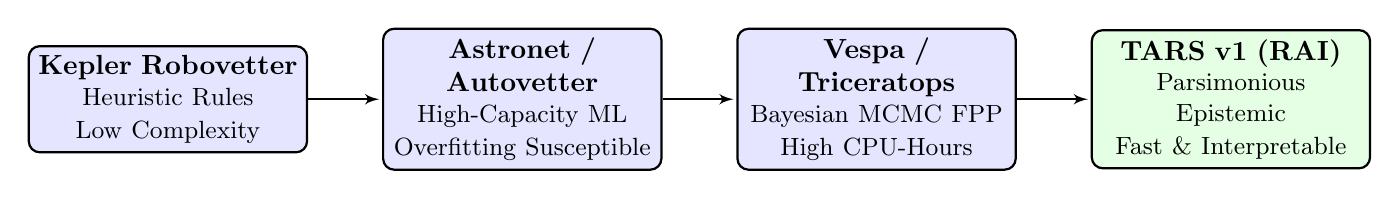
\begin{tikzpicture}[node distance=2.2cm, auto, >=latex', thick,
    block/.style={rectangle, draw, fill=blue!10, text width=3.3cm, text centered, rounded corners, minimum height=1.3cm},
    line/.style={draw, ->, shorten >=1pt}]
    
    \node [block] (robo) {
        \textbf{Kepler Robovetter}\\
        \small Heuristic Rules\\
        \small Low Complexity
    };
    \node [block, right of=robo, node distance=4.5cm] (ml) {
        \textbf{Astronet / Autovetter}\\
        \small High-Capacity ML\\
        \small Overfitting Susceptible
    };
    \node [block, right of=ml, node distance=4.5cm] (bayes) {
        \textbf{Vespa / Triceratops}\\
        \small Bayesian MCMC FPP\\
        \small High CPU-Hours
    };
    \node [block, right of=bayes, node distance=4.5cm, fill=green!10] (tars) {
        \textbf{TARS v1 (RAI)}\\
        \small Parsimonious Epistemic\\
        \small Fast \& Interpretable
    };
    
    \path [line] (robo) -- (ml);
    \path [line] (ml) -- (bayes);
    \path [line] (bayes) -- (tars);
\end{tikzpicture}
\caption{Historical evolution of automated exoplanet vetting methodologies, showing the progression from heuristic rules to modern parsimonious indexing.}
\label{fig:evolution}
\end{figure*}

\subsubsection{Rule-Based Heuristics}
The early Kepler pipelines utilized the Robovetter \citep{Coughlin2016}. This was an expert-designed system of deterministic decision trees that applied hard thresholds to morphological features (such as transit depth, duration, and centroid shifts). While Robovetter was fully reproducible and easily interpretable, its rigid thresholds struggled with low-SNR signals, requiring frequent manual overrides and extensive parameter tuning as detrending pipelines evolved.

\subsubsection{High-Capacity Machine Learning Ensembles}
To handle near-threshold detections, the community developed high-capacity classifiers. Autovetter \citep{McCauliff2015} introduced random forests to exoplanet vetting, utilizing dozens of engineered features. This was followed by deep learning approaches such as Astronet \citep{Shallue2018}, which employed 1D convolutional neural networks (CNNs) to classify phase-folded light curves directly. Subsequent architectures extended deep learning vetting to domain adaptation \citep{Ansdell2018}, multi-sector TESS classification \citep{Yu2019, Osborn2020, Olmschenk2021}, K2 discovery \citep{Dattilo2019}, and ensemble planet validation \citep{Armstrong2021}. While these classifiers improved ranking accuracy, they brought significant challenges:
\begin{itemize}
\item \textbf{Overfitting and Redundancy}: Ensembles typically utilize dozens of highly correlated features, making them susceptible to overfitting under dataset shift.
\item \textbf{Uncalibrated Output Probabilities}: High-capacity models frequently yield uncalibrated confidence scores \citep{Guo2017, Niculescu2005}, making it difficult for observers to interpret the outputs as true physical probabilities.
\item \textbf{Lack of Interpretability}: Deep neural networks behave as black boxes, providing no physical justification for candidate rejection.
\end{itemize}

\subsubsection{Bayesian Stellar Population Simulations}
To obtain physically meaningful probability estimates, Bayesian tools such as Vespa \citep{Morton2012, Morton2015, Morton2016}, PASTIS \citep{Diaz2014, Santerne2015}, BLENDER \citep{Torres2011}, and Triceratops \citep{Giacalone2021} calculate the False Positive Probability (FPP) of a candidate. They simulate millions of synthetic stellar populations (including blended background stars and orbiting binaries) to compute the relative likelihood of the data under different transit models. While highly rigorous, these tools are computationally expensive, requiring minutes to hours of CPU time per candidate. This creates a computational bottleneck when processing large-scale catalogs.

\subsection{The Transit Vetting Pipeline Flow and Bottlenecks} \label{sec:vetting_flow}
Automated vetting is not a single decision, but rather the culmination of a multi-stage data processing pipeline. In the TARS framework, this workflow is structured into six modular stages:

\begin{figure*}[htbp]
\centering
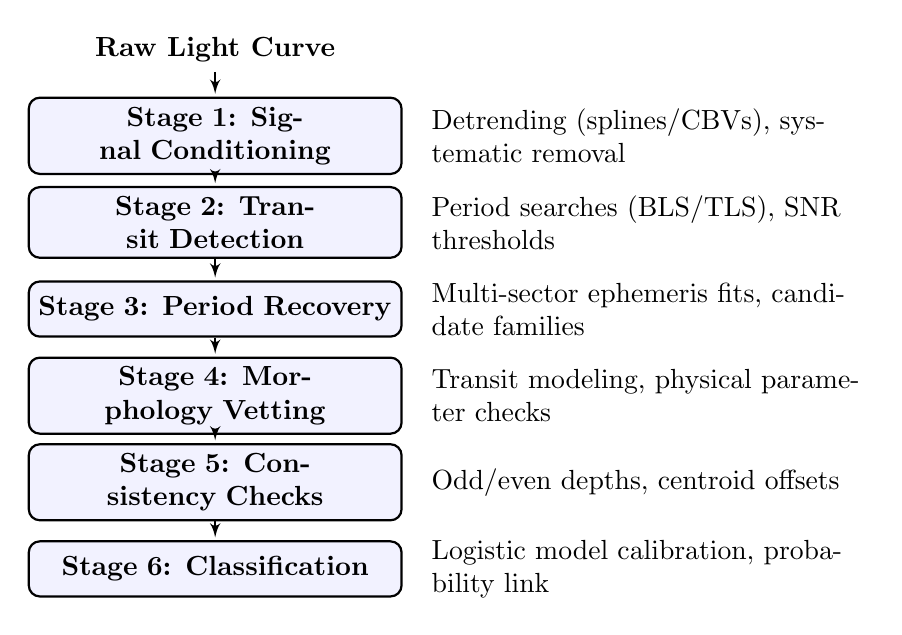
\begin{tikzpicture}[auto, >=latex', thick,
    block/.style={rectangle, draw, fill=blue!5, text width=4.5cm, text centered, rounded corners, minimum height=0.7cm},
    descr/.style={rectangle, text width=5.5cm, align=left, minimum height=0.7cm},
    line/.style={draw, ->, shorten >=1pt}]
    
    \node (raw) {\textbf{Raw Light Curve}};
    
    \node [block, below of=raw, node distance=1.1cm] (s1) {\textbf{Stage 1: Signal Conditioning}};
    \node [descr, right of=s1, node distance=5.5cm] (d1) {Detrending (splines/CBVs), systematic removal};
    
    \node [block, below of=s1, node distance=1.1cm] (s2) {\textbf{Stage 2: Transit Detection}};
    \node [descr, right of=s2, node distance=5.5cm] (d2) {Period searches (BLS/TLS), SNR thresholds};
    
    \node [block, below of=s2, node distance=1.1cm] (s3) {\textbf{Stage 3: Period Recovery}};
    \node [descr, right of=s3, node distance=5.5cm] (d3) {Multi-sector ephemeris fits, candidate families};
    
    \node [block, below of=s3, node distance=1.1cm] (s4) {\textbf{Stage 4: Morphology Vetting}};
    \node [descr, right of=s4, node distance=5.5cm] (d4) {Transit modeling, physical parameter checks};
    
    \node [block, below of=s4, node distance=1.1cm] (s5) {\textbf{Stage 5: Consistency Checks}};
    \node [descr, right of=s5, node distance=5.5cm] (d5) {Odd/even depths, centroid offsets};
    
    \node [block, below of=s5, node distance=1.1cm] (s6) {\textbf{Stage 6: Classification}};
    \node [descr, right of=s6, node distance=5.5cm] (d6) {Logistic model calibration, probability link};
    
    \path [line] (raw) -- (s1);
    \path [line] (s1) -- (s2);
    \path [line] (s2) -- (s3);
    \path [line] (s3) -- (s4);
    \path [line] (s4) -- (s5);
    \path [line] (s5) -- (s6);
\end{tikzpicture}
\caption{Modular layout of the 6-stage TARS automated exoplanet validation architecture, mapping data flow from raw flux inputs to final calibrated reliability probabilities.}
\label{fig:pipeline_flow}
\end{figure*}

The layout of the vetting architecture is summarized in Figure~\ref{fig:pipeline_flow}.
\begin{enumerate}
\item \textbf{Stage 1 (Signal Conditioning)}: Raw flux series are processed to remove long-term stellar rotational modulation and instrumental systematics \citep{Smith2012, Stumpe2012, Vanderburg2014, Luger2016, Luger2018, Aigrain2016}. This is achieved via high-pass filtering, iterative spline fitting, or projecting onto Co-trending Basis Vectors (CBVs). The conditioning stage must balance systematic removal against the preservation of long-period transits.
\item \textbf{Stage 2 (Transit Detection)}: The detrended light curve is searched for periodic transit signatures. Candidates are identified by finding the period $P$, epoch $T_0$, and duration $W$ that maximize the transit depth significance using algorithms such as BLS \citep{Kovacs2002} or TLS \citep{Hippke2019}.
\item \textbf{Stage 3 (Period Recovery \& Ephemeris Matching)}: Transit events from separate observation sectors or quarters are combined to fit a coherent linear ephemeris:
   \begin{equation}
   t_k = T_0 + k \cdot P
   \label{eq:ephemeris}
   \end{equation}
   This stage resolves the multi-peak periodogram structure \citep{Deeming1975, Roberts1987, Lomb1976, Scargle1982, VanderPlas2018, Dawson2010}, generating a list of candidate periods that match the observed transit timings.
\item \textbf{Stage 4 (Morphological Vetting)}: The light curve is folded at the candidate period and fitted with an analytical transit model \citep{Mandel2002, Gimenez2006, Kreidberg2015, Seager2003} to derive physical parameters, including the ratio of planet radius to stellar radius $R_p/R_*$, semi-major axis $a/R_*$, and impact parameter $b$.
\item \textbf{Stage 5 (Consistency Validation)}: Checks are executed to identify eclipsing binaries, such as comparing the depths of odd and even transits (which differ for eclipsing binaries with eccentric orbits or different secondary components) and measuring centroid offsets during transit to locate the true source of the dip.
\item \textbf{Stage 6 (Probabilistic Classification)}: Feature vectors containing metrics from all previous stages are fed into machine learning classifiers to predict the probability of the candidate being a true planet, evaluated via diagnostic metrics such as AUROC, AUPRC, DeLong statistics \citep{DeLong1988}, Youden's J index \citep{Youden1950}, and Matthews Correlation Coefficient \citep[MCC;][]{Matthews1975}.
\end{enumerate}

\subsection{Stellar Activity and Vetting Degeneracy} \label{sec:stellar_activity}
The primary astrophysical bottleneck in transit vetting is stellar activity. Active stars exhibit magnetic starspots on their photospheres \citep{Meunier2010, Aigrain2012}. As the star rotates, these spot groups cross the visible stellar hemisphere, causing quasi-periodic flux variations at the stellar rotation period $P_{\text{rot}}$ and its harmonics \citep{McQuillan2013, McQuillan2014, Reinhold2013}. Furthermore, starspot groups grow and decay on timescales of days to weeks, introducing amplitude and phase variations in the light curve.

This magnetic variability introduces two major challenges for transit detection:
\begin{enumerate}
\item \textbf{False Transits}: The spot groups and active regions can create temporary, localized flux dips that resemble transits when observed over a short baseline.
\item \textbf{Alias Frequency Clustering}: On active stars, stellar rotation creates quasi-periodic flux dips that can alias (fold) onto the true planetary transit period \citep{Dawson2010}. When performing transit searches, the algorithm cannot easily distinguish the true transit signal from stellar rotation harmonics ($P_{\text{rot}}/2, 2 P_{\text{rot}}$, etc.), producing multiple false candidate period peaks that survive standard vetting checks.
\end{enumerate}

When a transit search algorithm folds the light curve at these incorrect alias periods, the resulting phase-folded light curve can exhibit a high signal-to-noise ratio, confusing classical classifiers. The number of candidate periods that survive initial checks---often termed ``candidate branching'' or ``alias explosion''---increases exponentially, creating high signal recovery ambiguity.

\subsection{Aleatoric vs. Epistemic Uncertainty in Exoplanet Vetting} \label{sec:uncertainty_types}
To build robust classifiers, it is essential to distinguish between two types of uncertainty:
\begin{itemize}
\item \textbf{Aleatoric Uncertainty}: This represents the physical randomness inherent in the astronomical source. In vetting, it corresponds to whether the physical source is a planet, an eclipsing binary, or a blended background binary. This uncertainty is driven by physical degeneracies (e.g., a small star eclipsing a large star can produce the same transit depth as a planet transiting a Sun-like star) and is typically modeled using Bayesian false positive probability (FPP) packages like \texttt{vespa} \citep{Morton2012, Morton2015}.
\item \textbf{Epistemic Uncertainty}: This represents the uncertainty associated with the signal recovery process itself under noise and activity. It answers the question: \textit{How reliably can we recover the true period and ephemeris of the candidate given the observation window and the stellar activity profile?}
\end{itemize}

Many existing vetting pipelines primarily optimize classification performance rather than explicitly separating epistemic recovery ambiguity from astrophysical false-positive probability. They construct classifiers containing up to dozens of correlated features (such as ``family complexity'', which counts raw alias frequencies and periodogram peaks) to predict the class label $P(\text{Planet} \mid X)$. Because these classifiers are fit on historical catalogs, they are highly sensitive to dataset selection biases and cannot trace \textit{why} a candidate is flagged as ambiguous.

\subsection{Operationalizing a Multi-Dimensional Validation Protocol} \label{sec:contribution}

To address the limitations of conventional exoplanet vetting evaluations, this work operationalizes and evaluates a reproducible, multi-dimensional validation protocol for ambiguity-aware transit-vetting pipelines. Rather than evaluating a classifier solely on a single, local train/test split, our protocol establishes a multi-layered certification hierarchy (Figure~\ref{fig:validation_hierarchy}) designed to expose hidden operational limits, calibration decay under domain shifts, and statistical redundancies.

\begin{figure*}[htbp]
\centering
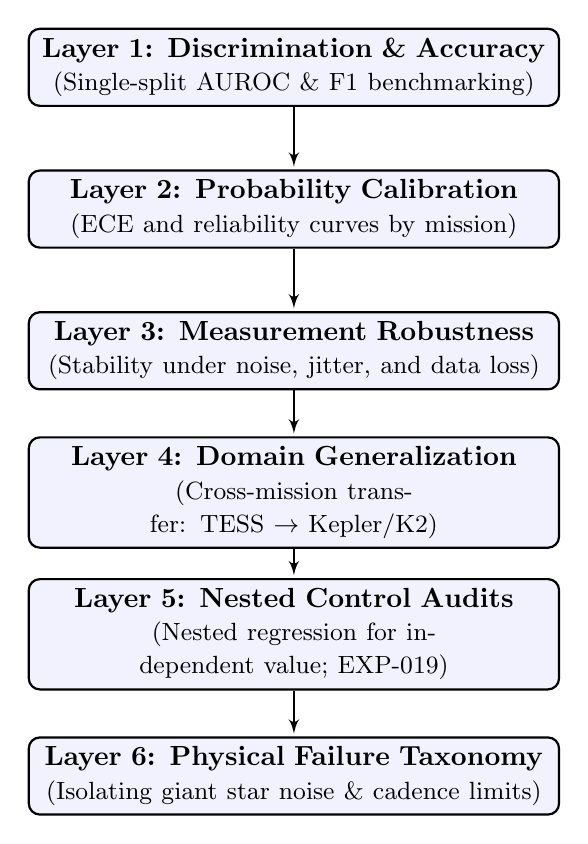
\begin{tikzpicture}[node distance=1.5cm, auto, >=latex', thick,
    block/.style={rectangle, draw, fill=blue!5, text width=6.5cm, text centered, rounded corners, minimum height=0.9cm},
    line/.style={draw, ->, shorten >=1pt}]
    
    \node [block] (acc) {\textbf{Layer 1: Discrimination \& Accuracy} \\ \small (Single-split AUROC \& F1 benchmarking)};
    \node [block, below of=acc, node distance=1.8cm] (cal) {\textbf{Layer 2: Probability Calibration} \\ \small (ECE and reliability curves by mission)};
    \node [block, below of=cal, node distance=1.8cm] (rob) {\textbf{Layer 3: Measurement Robustness} \\ \small (Stability under noise, jitter, and data loss)};
    \node [block, below of=rob, node distance=1.8cm] (dom) {\textbf{Layer 4: Domain Generalization} \\ \small (Cross-mission transfer: TESS $\rightarrow$ Kepler/K2)};
    \node [block, below of=dom, node distance=1.8cm] (nest) {\textbf{Layer 5: Nested Control Audits} \\ \small (Nested regression for independent value; EXP-019)};
    \node [block, below of=nest, node distance=1.8cm] (fail) {\textbf{Layer 6: Physical Failure Taxonomy} \\ \small (Isolating giant star noise \& cadence limits)};
    
    \path [line] (acc) -- (cal);
    \path [line] (cal) -- (rob);
    \path [line] (rob) -- (dom);
    \path [line] (dom) -- (nest);
    \path [line] (nest) -- (fail);
    
\end{tikzpicture}
\caption{The Multi-Dimensional Validation Hierarchy. Exoplanet vetting systems must be certified across all six layers of this protocol to ensure scientific reliability, going beyond standard single-split AUROC testing. Each certification layer maps directly to our 13 coordinated validation experiments (Section~\ref{sec:method_experiment_matrix}, Table~\ref{tab:experiment_master_matrix}): Layer 1 (Discrimination \& Accuracy): EXP-001, EXP-004, EXP-005, EXP-011, EXP-012; Layer 2 (Probability Calibration): EXP-007, EXP-009, EXP-011; Layer 3 (Measurement Robustness): EXP-007, EXP-023; Layer 4 (Domain Generalization): EXP-013; Layer 5 (Nested Control Audits): EXP-019; Layer 6 (Physical Failure Taxonomy): EXP-002, EXP-003, and host-star cohort partitioning.}
\label{fig:validation_hierarchy}
\end{figure*}

Under this protocol, we evaluate the Transit Ambiguity Recovery System (TARS) as a baseline case study. TARS employs a graph-theoretic Recovery Ambiguity Index (RAI) constructed as a parsimonious, signed sum of five standardized graph-theoretic and harmonic features derived from information theory \citep{Shannon1948, Cover2006}. To execute this multi-layer audit systematically, our study operationalizes a coordinated suite of 13 executed validation experiments selected from our 23-stage preregistered experimental registry (spanning designations EXP-001 through EXP-023, with intermediate numbers corresponding to internal engineering calibrations and exploratory runs archived during pipeline development; fully cataloged in Section~\ref{sec:method_experiment_matrix}, Table~\ref{tab:experiment_master_matrix}), spanning full-scale production runs, synthetic injection sweeps, nested feature audits, and cross-mission stress tests. We deploy this validation protocol to evaluate TARS on unblinded cohorts from TESS, Kepler, and K2 ($N=1780$, $100$, and $41$ respectively), showing that while TARS achieves comparable discrimination to complex stacks on standard splits, our multi-dimensional auditing successfully diagnoses its operational limits:
\begin{itemize}
    \item \textbf{Out-of-Domain Collapse}: Evaluating on Kepler long-cadence data reveals a collapse in ranking performance ($\text{AUROC} \approx 0.48$) and severe calibration decay (ECE $= 0.5212$), tracing a physical sensitivity limit induced by cadence-driven transit-edge blurring.
    \item \textbf{Nested Controls}: Nested regression controls (EXP-019; Section~\ref{sec:results_exp019}) expose that the graph-theoretic RAI lacks statistically significant independent predictive value once controlling for BLS SDE, directly identifying a feature redundancy that conventional evaluations fail to detect.
    \item \textbf{Cohort Boundaries}: Subgroup partitioning isolates stellar convective noise on giant hosts ($\log g < 4.0$) as a physical boundary deforming graph topology, defining where the classifier fails.
\end{itemize}

By proposing and testing this protocol, we demonstrate that rigorous evaluation can systematically reveal hidden limitations in exoplanet vetting pipelines, providing a reusable framework for certifying future automated search engines before large-scale production deployment.

\section{Related Work} \label{sec:related_work}

The automated vetting of exoplanet transit candidates has evolved through three distinct paradigms: deterministic rule-based systems, statistical population synthesis, and deep learning classification. This section reviews these paradigms, details their physical and statistical assumptions, and positions the TARS v1 framework within the literature.

\subsection{Rule-Based Heuristic Vetting} \label{sec:heuristic_vetting}
Early wide-field transit surveys relied on deterministic, rule-based decision trees to filter out false positives. The primary reference for this approach is Kepler’s Robovetter \citep{Coughlin2016, Thompson2018}. Robovetter evaluates Threshold Crossing Events (TCEs) by passing them through a series of sequential tests, checking for:
\begin{itemize}
\item Data quality flag anomalies (e.g., pointing offsets and cosmic ray hits).
\item Inherent signal consistency, such as comparing the depth of odd and even transits to identify eclipsing binaries.
\item The presence of secondary eclipses, which indicates a stellar or substellar companion rather than a planet.
\item Individual transit morphology fits to ensure the transit shape matches a physical light curve model \citep{Mandel2002}.
\end{itemize}

Although Robovetter is computationally efficient and highly interpretable, its inputs are pre-filtered by hard detection threshold boundaries (such as the Kepler pipeline's detection threshold requiring $\text{SNR} \ge 7.1$ \citealt{Jenkins2010}). Marginal candidates falling just below these thresholds are rejected without any quantification of the surrounding uncertainty. This rigidity limits its ability to handle signals near the detection limit or in the presence of complex stellar activity.

\subsection{Statistical Validation and False Positive Probability (FPP)} \label{sec:statistical_validation}
To address the limitations of binary classification, statistical validation frameworks were developed to calculate the False Positive Probability (FPP) of individual candidates. The leading tools are Vespa \citep{Morton2012, Morton2015} and Triceratops \citep{Giacalone2021}.

Vespa computes the FPP by performing Bayesian model comparison, evaluating the relative likelihood of the observed transit shape under multiple astronomical scenarios:
\begin{enumerate}
\item A transiting planet around the target star.
\item A blended eclipsing binary (BEB) in the background.
\item A bound eclipsing binary companion (HEB).
\item A companion star with a transiting planet.
\end{enumerate}

Triceratops extends this methodology by incorporating spatial priors from nearby stellar catalogs, which is particularly important for TESS due to its large pixel scale ($21''$ per pixel) where flux contamination is common.

These validation models focus on \textbf{aleatoric uncertainty}---specifically, the physical source degeneracy (i.e., whether the physical source causing the dip is a planet or a binary companion). However, they do not address \textbf{epistemic uncertainty}---the recovery ambiguity of the signal itself under non-stationary noise or stellar activity. They assume that the detected period and transit shape are correct and do not model the likelihood of the recovery pipeline locking onto incorrect alias periods. Furthermore, these tools are computationally intensive, requiring external stellar population simulations.

\subsection{Deep Learning and Dimensionality Reduction Vetting} \label{sec:deep_learning_vetting}
With the explosion of data from surveys, machine learning models have been deployed to automate classification. The most notable implementation is Astronet \citep{Shallue2018}, a deep convolutional neural network (CNN) that classifies TCEs using 1D light curve representations. Other models, such as DAVE \citep{Kostov2019}, incorporate non-linear feature embeddings and centroid motion analysis to improve classification accuracy.

Deep neural networks achieve high predictive performance on validation sets. However, they act as black-box estimators, making it difficult to trace why specific candidates are rejected. Furthermore, deep classifiers are prone to overconfidence and calibration decay under dataset shifts \citep{Guo2017}. Post-hoc calibration techniques, such as temperature scaling, ensemble models, or post-hoc binning, have been investigated to mitigate this issue. However, if a model trained on quiet stars is applied to highly active stars, the predicted class probabilities $P(\text{Planet} \mid X)$ still fail to reflect the increased signal recovery ambiguity, leading to high false positive rates.

\subsection{Novelty Positioning: Signal Ambiguity vs. Classification Probability} \label{sec:novelty_positioning}
TARS v1 addresses one limitation not explicitly addressed in previous work: the conflation of classification probability with recovery ambiguity. Traditional classifiers output a probability $P(\text{Planet} \mid X)$, which is sensitive to training class distributions and dataset selection biases.

In contrast, the Recovery Ambiguity Index (RAI) measures the epistemic uncertainty of the signal itself: \textit{How easily is the signal's period and morphology confused with stellar rotation, harmonics, or random noise regimes?}

By computing features like period uniqueness, candidate concentration, and graph clustering of alias frequencies, the RAI quantifies the inherent ambiguity in the transit detection workflow. This provides a highly parsimonious (1 derived index), well-calibrated (ECE = 0.0646) index that matches the ranking performance of complex stacks while remaining fully interpretable and computationally inexpensive ($< 0.1$ s execution time).

\begin{deluxetable*}{llllll}
\tabletypesize{\footnotesize}
\tablecaption{Novelty Matrix Comparison\label{tab:novelty}}
\tablewidth{0pt}
\tablehead{
\colhead{Dimension} & \colhead{Robovetter} & \colhead{Vespa} & \colhead{Triceratops} & \colhead{Astronet} & \colhead{TARS v1 (This Work)}
}
\startdata
\textbf{Primary Goal} & Automated threshold vetting & Statistical FPP & FPP under blends & \parbox{2.2cm}{CNN classification of TCEs} & \parbox{3.5cm}{Quantify signal recovery ambiguity} \\
\textbf{Core Metric} & Decision tree flags & FPP point estimate & FPP and Nearby FPP & \parbox{2.2cm}{Probabilistic class prediction} & \parbox{3.5cm}{\textbf{Recovery Ambiguity Index (RAI)}} \\
\textbf{Uncertainty Type} & None (Deterministic) & \parbox{2.2cm}{Aleatoric (Blend likelihoods)} & \parbox{2.2cm}{Aleatoric (Bayesian blend models)} & \parbox{2.2cm}{Aleatoric (Softmax output)} & \parbox{3.5cm}{\textbf{Epistemic (Vetting process degeneracy)}} \\
\textbf{Astrophysical Focus} & Instrument anomalies & \parbox{2.2cm}{Stellar population synthesis} & \parbox{2.2cm}{Background EB contamination} & \parbox{2.2cm}{Transit shape morphology} & \parbox{3.5cm}{\textbf{Stellar activity \& period stability}} \\
\textbf{Computational Footprint} & Low & \parbox{2.2cm}{Medium (minutes/candidate)} & \parbox{2.2cm}{High (hours/candidate)} & \parbox{2.2cm}{High (GPU needed)} & \parbox{3.5cm}{\textbf{Very Low ($RAI$ calculation requires $< 0.1$ s, $O(N^2)$ complexity)}} \\
\enddata
\end{deluxetable*}

\subsection{Prior Vetting Stage Context} \label{sec:prior_stages}
To understand how TARS v1 integrates with current automated pipelines, we must examine its dependency on Stages 1 and 2 of the exoplanet pipeline:
\begin{itemize}
\item \textbf{Stage 1 (Signal Conditioning) Operating Boundaries}: Detrending algorithms typically use high-pass filters or smoothing splines with a fixed window length (or knot spacing) to remove low-frequency stellar activity. If this window is too narrow, the planet transits themselves are attenuated, introducing false morphological variations. If the window is too wide, residual stellar activity remains, deforming the transit profile and generating harmonic period aliases.
\item \textbf{Stage 2 (Transit Detection) Operating Limits}: The Box Least Squares (BLS) and Transit Least Squares (TLS) algorithms identify periodic signals by searching a grid of test periods. When the signal is weak (near the detection threshold of $\text{SDE} < 6.0$), the periodogram contains multiple competing peaks due to noise fluctuations. When the stellar noise is active and non-white (e.g. convective granulation), these peaks cluster near rotation harmonics. Traditional pipelines attempt to classify each peak independently, ignoring the global network structure of these aliases. TARS v1 directly addresses this by building a graph of these competing period peaks to evaluate signal uniqueness.
\end{itemize}

\section{Methodology: Isolating Recovery Ambiguity} \label{sec:methodology}

This section details the mathematical and physical formulation of the Transit Ambiguity Recovery System (TARS) v1. The primary objective of this methodology is to isolate and quantify \textbf{epistemic uncertainty} (signal recovery ambiguity) during transit vetting, separating it from \textbf{aleatoric uncertainty} (astrophysical source degeneracy).

\subsection{Scientific Objective and Vetting Pipeline Flow} \label{sec:method_pipeline_flow}
In wide-field space photometry, the transit signal of a true exoplanet is easily obscured by non-stationary noise, instrumental systematics, and stellar rotation. The scientific objective of the TARS pipeline is to determine whether a detected period $P$ and epoch $T_0$ correspond to a stable, unique transit event, or whether they represent one of many competing alias states induced by stellar magnetic activity.

The global TARS pipeline is structured into six modular stages. The design rationale, inputs, outputs, assumptions, and failure modes for each stage are detailed below:
\begin{itemize}
\item \textbf{Stage 1: Signal Conditioning}
    \begin{itemize}
    \item \textit{Inputs}: Raw flux time-series $f(t)$
    \item \textit{Outputs}: Detrended flux series $f_{\text{det}}(t)$
    \item \textit{Scientific Objective}: Remove low-frequency stellar activity trends (such as rotational modulation) and instrumental systematics (such as thermal drifts).
    \item \textit{Assumptions}: Stellar activity variations and instrumental systematics vary on timescales significantly longer than the transit duration (typically $\tau_{\text{noise}} > 1$ day vs. $\tau_{\text{transit}} < 6$ hours).
    \item \textit{Failure Modes}: If the detrending filter or spline window is too narrow, the planet transits themselves are attenuated, introducing false morphological variations. If the window is too wide, residual stellar activity remains, deforming the transit profile and generating harmonic period aliases.
    \end{itemize}
\item \textbf{Stage 2: Transit Detection}
    \begin{itemize}
    \item \textit{Inputs}: Detrended flux $f_{\text{det}}(t)$
    \item \textit{Outputs}: Threshold Crossing Events (TCEs) with top period $P_{\text{top}}$, epoch $T_0$, and duration $W$
    \item \textit{Scientific Objective}: Search the period-epoch-duration parameter grid to identify periodic brightness dips.
    \item \textit{Assumptions}: Residual noise after detrending is white Gaussian noise, and transit events are strictly periodic.
    \item \textit{Failure Modes}: Signals with highly eccentric orbits (long durations relative to period) or single-transit events are missed.
    \end{itemize}
\item \textbf{Stage 3: Period Recovery}
    \begin{itemize}
    \item \textit{Inputs}: TCE, sector-level partitions of $f_{\text{det}}(t)$
    \item \textit{Outputs}: Surviving candidate periods set $\mathcal{P} = \{P_c\}$
    \item \textit{Scientific Objective}: Verify the stability and uniqueness of the period recovery search across independent observation epochs.
    \item \textit{Assumptions}: Transit timings follow a coherent linear ephemeris across all sectors.
    \item \textit{Failure Modes}: Severe Transit Timing Variations (TTVs) or wide data gaps prune valid periods.
    \end{itemize}
\item \textbf{Stage 4: Morphology Vetting}
    \begin{itemize}
    \item \textit{Inputs}: Folded light curve for each $P_c$
    \item \textit{Outputs}: Mandel \& Agol transit model fits ($R_p/R_*$, $a/R_*$, $b$)
    \item \textit{Scientific Objective}: Derive physical transit parameters and evaluate transit shape consistency.
    \item \textit{Assumptions}: Spherically symmetric star and planet, circular orbit, and quadratic limb darkening.
    \item \textit{Failure Modes}: Photospheric spot crossings deform transit shapes and bias derived parameters.
    \end{itemize}
\item \textbf{Stage 5: Consistency Checks}
    \begin{itemize}
    \item \textit{Inputs}: Model parameters, transit flux series
    \item \textit{Outputs}: Centroid offsets, odd/even depth differences
    \item \textit{Scientific Objective}: Identify eclipsing binaries and background contaminants.
    \item \textit{Assumptions}: Instrumental pointing and pixel response are stable during transit epochs.
    \item \textit{Failure Modes}: Crowded fields mix centroid shifts, causing false positive errors.
    \end{itemize}
\item \textbf{Stage 6: Classification}
    \begin{itemize}
    \item \textit{Inputs}: Recovery Ambiguity Index (RAI)
    \item \textit{Outputs}: Light curve reliability probability $P(Y=1 \mid z_{\text{RAI}})$
    \item \textit{Scientific Objective}: Provide a calibrated probability of candidate reliability based on signal recovery ambiguity.
    \item \textit{Assumptions}: Feature distributions are logistically calibrated.
    \item \textit{Failure Modes}: Out-of-distribution (OOD) stellar cohorts degrade calibration.
    \end{itemize}
\end{itemize}

\subsection{Operational Dataset Construction and Partitioning} \label{sec:method_dataset_overview}

To ensure reproducibility, we detail the construction of the exoplanet dataset and the partitions used for model fitting, parameter tuning, and independent evaluation. 

\begin{itemize}
\item \textbf{Data Acquisition and Preprocessing}: Raw light curves are acquired from the Mikulski Archive for Space Telescopes (MAST) for targets observed by the Transiting Exoplanet Survey Satellite (TESS). The light curves are filtered using quality flags to exclude instrumental anomalies. Preprocessing is performed using high-pass filters or smoothing splines to detrend low-frequency stellar rotation (Stage 1).
\item \textbf{Candidate Generation and Vetting}: Transit detection (Stage 2) is executed via Box Least Squares (BLS) and Transit Least Squares (TLS) grid searches to produce Threshold Crossing Events (TCEs) with candidate periods and epochs. Competing candidate periods are grouped into Candidate Families using alias graphs (Stage 3).
\item \textbf{Label Assignment}: Ground-truth labels are mapped from the NASA Exoplanet Archive and the TESS Follow-up Observing Program Working Group (TFOP WG). True planets are designated as \texttt{Tier A} (positive class, $Y=1$) and confirmed false positives are designated as \texttt{Tier C} (negative class, $Y=0$).
\item \textbf{Dataset Partitioning}: The dataset is partitioned into distinct regimes as detailed in Table~\ref{tab:dataset_overview}. The progression of data through these partitions is illustrated in Figure~\ref{fig:dataset_workflow}. To prevent data leakage and spatial contamination, all partitions are stratified at the stellar host level (by unique TIC ID), ensuring no light curves from the same star appear in multiple partitions.
\item \textbf{Reproducibility}: The code, frozen standardization parameters, and validation scripts are version-controlled and publicly available at \url{https://github.com/rk-roshan-kr/Tars-Transit-Ambiguity-Recovery-System}, with all random seeds locked to \texttt{42}.
\end{itemize}

\begin{table*}[htbp]
\centering
\caption{Dataset Partitions, Label Provenance, and Class Balance}
\label{tab:dataset_overview}
\begin{tabular}{llcccclcc}
\hline\hline
Partition & Role & Unique Stars & Light Curves & Label Provenance & $N_{\text{Planets}}$ & $N_{\text{FPs}}$ & Class Bal. \\
\hline
TRAIN & Model fitting & 408 & 1,253 & Mixed (NASA Archive + TFOP WG) & 749 & 504 & 59.78\% \\
VALIDATION & Hyperparameter tuning & 47 & 105 & Mixed (NASA Archive + TFOP WG) & 62 & 43 & 59.05\% \\
BLIND & Independent evaluation & 60 & 175 & Mixed (NASA Archive + TFOP WG) & 102 & 73 & 58.29\% \\
\hline
TARS-250K-R1 & Operational (unlabeled) & 129,383 & 250,010 & None & N/A & N/A & N/A \\
\hline
\end{tabular}
\end{table*}


\begin{figure*}[htbp]
\centering
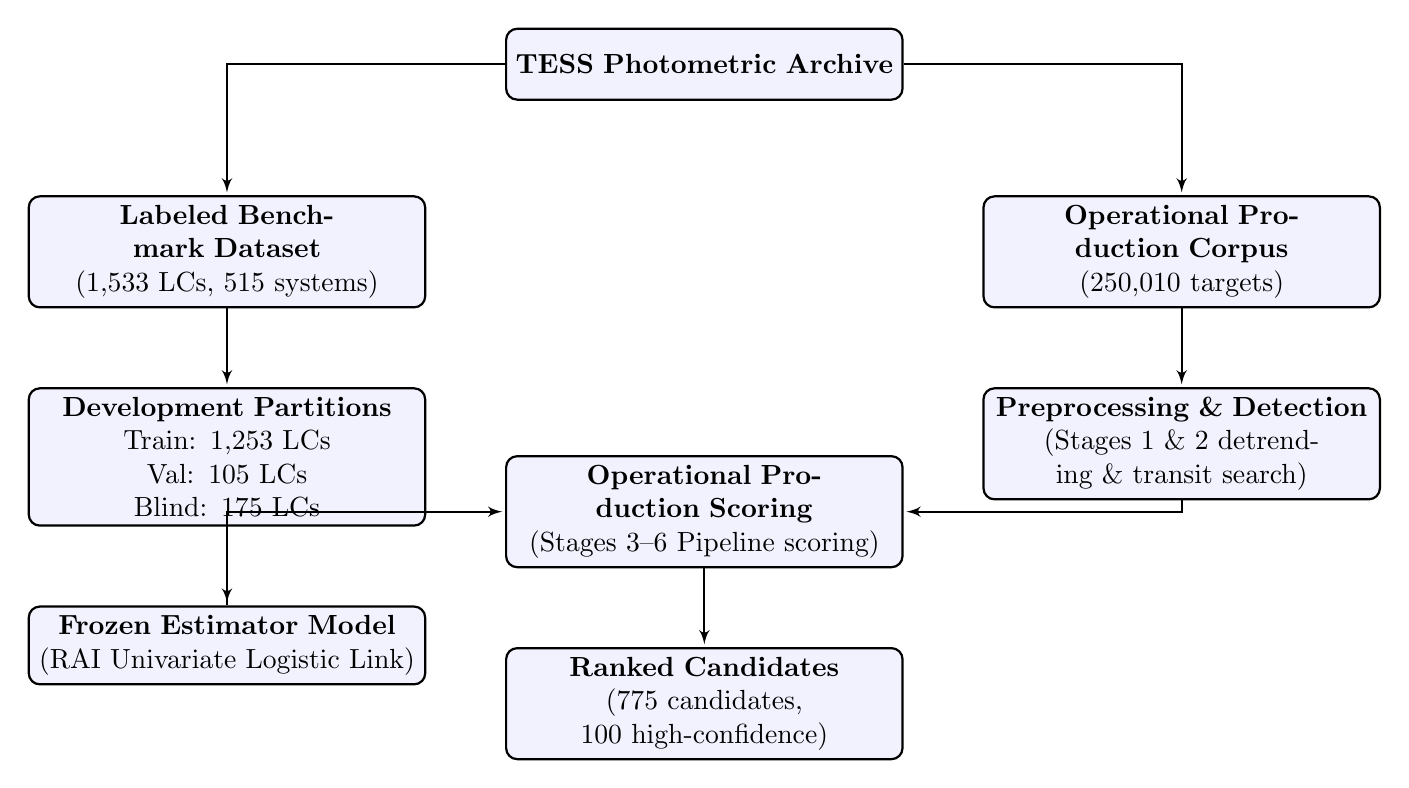
\begin{tikzpicture}[auto, >=latex', thick,
    block/.style={rectangle, draw, fill=blue!5, text width=4.8cm, text centered, rounded corners, minimum height=0.9cm},
    line/.style={draw, ->, shorten >=1pt}]
    
    % Top Level
    \node [block] (tess) {\textbf{TESS Photometric Archive}};
    
    % Parallel Paths
    \node [block, below left=1.2cm and 1.0cm of tess] (benchmark) {\textbf{Labeled Benchmark Dataset} \\ (1,533 LCs, 515 systems)};
    \node [block, below right=1.2cm and 1.0cm of tess] (ops) {\textbf{Operational Production Corpus} \\ (250,010 targets)};
    
    % Benchmark Splits
    \node [block, below=1.0cm of benchmark] (splits) {\textbf{Development Partitions} \\ Train: 1,253 LCs \\ Val: 105 LCs \\ Blind: 175 LCs};
    
    % Model Dev
    \node [block, below=1.0cm of splits] (model) {\textbf{Frozen Estimator Model} \\ (RAI Univariate Logistic Link)};
    
    % Ingestion
    \node [block, below=1.0cm of ops] (ingest) {\textbf{Preprocessing \& Detection} \\ (Stages 1 \& 2 detrending \& transit search)};
    
    % Merge/Deployment
    \node [block, below=4.5cm of tess] (scoring) {\textbf{Operational Production Scoring} \\ (Stages 3--6 Pipeline scoring)};
    
    % Output
    \node [block, below=1.0cm of scoring] (output) {\textbf{Ranked Candidates} \\ (775 candidates, 100 high-confidence)};
    
    % Paths
    \path [line] (tess) -| (benchmark);
    \path [line] (tess) -| (ops);
    \path [line] (benchmark) -- (splits);
    \path [line] (splits) -- (model);
    \path [line] (ops) -- (ingest);
    \path [line] (model) |- (scoring);
    \path [line] (ingest) |- (scoring);
    \path [line] (scoring) -- (output);
    
\end{tikzpicture}
\caption{Workflow diagram separating model development from operational production deployment. The TESS Photometric Archive branches into: (left) the Labeled Benchmark Dataset, which is partitioned into training, validation, and blind evaluation subsets to optimize and freeze the univariate RAI model; and (right) the unlabeled Operational Production Corpus. Both branches merge at the operational production scoring stage, where the frozen RAI model is deployed to generate the final ranked candidate catalog.}
\label{fig:dataset_workflow}
\end{figure*}

The statistical evaluation presented in Section~\ref{sec:results} is intentionally restricted to the labeled blind validation partition. Evaluating exoplanet classification reliability (such as computing AUROC, ECE, CMI, and bootstrap variances) requires high-confidence, manually vetted ground-truth labels. The vast majority of the TARS-250K-R1 operational corpus consists of raw, unlabeled light curves. Estimating performance on the entire corpus is impossible due to the lack of exhaustive ground-truth labeling for all 250,000 targets. By evaluating performance exclusively on the independent, strictly labeled blind validation partition, we guarantee that the calculated metrics represent true classification capabilities, while the production pipeline operates across the entire unlabeled corpus to score and rank candidates in a search for new discovery targets.

\subsection{Stage 3 Period Recovery and Candidate Family Construction} \label{sec:method_candidate_family}
Stellar activity introduces magnetic starspots that rotate with the stellar surface, causing quasi-periodic modulation at the stellar rotation period $P_{\text{rot}}$ and its harmonics. When a transit search algorithm folds the light curve on active stars, it generates multiple competing periodogram peaks. Stage 3 of TARS resolves this degeneracy by constructing \textbf{Candidate Families}.

The algorithm for candidate family construction is executed through the following sequential steps:
\begin{enumerate}
\item \textbf{Grid Search and Peak Extraction}: A Box Least Squares \citep[BLS;][]{Kovacs2002} search scan is run across the detrended light curve $f_{\text{det}}(t)$ to identify all local periodogram power peaks exceeding the detection threshold. This yields a raw candidate period set $\mathcal{P}_{\text{raw}}$.
\item \textbf{Multi-Sector Epoch Verification}: The light curve is split into independent observation sectors (or equal-length time partitions). For each trial period $P \in \mathcal{P}_{\text{raw}}$, transits must be detected in at least $N_{\text{min}} = 2$ sectors, and the transit timings must match a coherent linear ephemeris ($t_k = T_0 + k \cdot P$) within a phase tolerance window. Periods failing this timing check are pruned.
\item \textbf{Harmonic Matching}: Every pair of surviving periods $(P_i, P_j)$ is compared to evaluate if their ratio is close to an integer ratio. We define a harmonic edge between them if:
    \begin{equation}
    \min_{r \in \{2, 3, 4, 5\}} \left| \frac{P_i}{P_j} - r \right| < \epsilon \quad \text{or} \quad \left| \frac{P_j}{P_i} - r \right| < \epsilon
    \label{eq:harmonic_edge}
    \end{equation}
    where the tolerance is set to $\epsilon = 0.05$.
\item \textbf{Alias Graph Construction}: An undirected graph $G = (V, E)$ is built, where the vertices $V$ represent the surviving candidate periods, and the edges $E$ represent verified harmonic connections.
\item \textbf{Connected Component Extraction}: The graph $G$ is partitioned into its connected components (subgraphs). The component containing the top consensus-ranked period $P_{\text{top}}$ is extracted as the \textbf{Candidate Family} representing the target. The number of nodes in this subgraph is $N_{\text{final}}$.
\end{enumerate}

\begin{figure}[htbp]
\centering
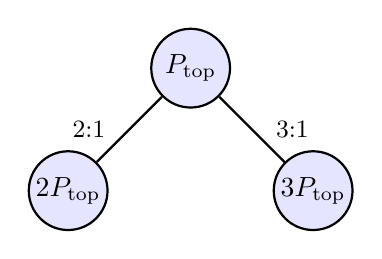
\begin{tikzpicture}[node distance=1.5cm, auto, >=latex', thick,
    every node/.style={circle, draw, fill=blue!10, minimum size=1.0cm, inner sep=0pt}]
    
    \node (ptop) {$P_{\text{top}}$};
    \node [below left of=ptop, node distance=2.2cm] (p2ptop) {$2 P_{\text{top}}$};
    \node [below right of=ptop, node distance=2.2cm] (p3ptop) {$3 P_{\text{top}}$};
    
    \path[draw] (ptop) -- node[left,draw=none,fill=none] {\small 2:1} (p2ptop);
    \path[draw] (ptop) -- node[right,draw=none,fill=none] {\small 3:1} (p3ptop);
\end{tikzpicture}
\caption{Representation of an exoplanet candidate alias graph. Vertices denote period hypotheses, and edges represent matched harmonics within phase tolerance $\epsilon = 0.05$.}
\label{fig:alias_graph}
\end{figure}

\subsection{Derivation of the Five RAI Sub-Features} \label{sec:method_features}
To quantify the topological properties of the alias graph and the stability of the period recovery search, TARS computes five sub-features from the candidate period set $\mathcal{P}$:

\subsubsection{Stability ($x_{\text{stab}}$)}
Stability measures the complexity of the surviving candidate family. It is defined as the total count of surviving candidates that match the epoch timings across all observation partitions:
\begin{equation}
x_{\text{stab}} = N_{\text{final}}
\label{eq:stab}
\end{equation}
\begin{itemize}
\item \textbf{Motivation}: Real planets produce highly stable detections that lock onto a single period, whereas stellar active hosts yield multiple competing peaks.
\item \textbf{Physical Intuition}: A clean transit signal in a quiet star will yield a single stable peak ($N_{\text{final}} = 1$). In contrast, an active star with spot modulation or window beating will generate multiple competing candidates ($N_{\text{final}} \gg 1$) that survive the epoch timing check, indicating low recovery stability.
\item \textbf{Failure Modes}: Severe data gaps or timing variations can artificially prune valid candidate periods, lowering the value.
\end{itemize}

\subsubsection{Graph Entropy ($x_{\text{ent}}$)}
Graph entropy measures the structural complexity and dispersion of the alias network. Let $d_k$ be the degree of vertex $k$ in the alias graph $G$. We compute the normalized degree probability $p_k = d_k / \sum_{j} d_j$. The Shannon graph entropy $x_{\text{ent}}$ is defined as:
\begin{equation}
x_{\text{ent}} = H_D = -\sum_{k=1}^{N_{\text{final}}} p_k \log_2 p_k
\label{eq:entropy}
\end{equation}
If a vertex has degree zero, we define $0 \log_2 0 = 0$.
\begin{itemize}
\item \textbf{Motivation}: Captures the degree of structure or randomness in the alias distribution.
\item \textbf{Physical Intuition}: If the alias periods are tightly organized around a central harmonic hub (e.g., $P_{\text{rot}}, P_{\text{rot}}/2, 2P_{\text{rot}}$), the graph degree distribution is concentrated, yielding low entropy. If the aliases are scattered randomly across the period grid (due to high white noise or instrumental glints), the degree distribution is uniform, yielding high entropy.
\item \textbf{Failure Modes}: Highly sparse graphs can yield undefined or unstable entropy estimates.
\end{itemize}

\subsubsection{Harmonic Density ($x_{\text{dens}}$)}
Harmonic density counts the number of competing candidate periods that lie close to an integer ratio or harmonic of the top candidate period $P_{\text{top}}$. It is defined as:
\begin{equation}
x_{\text{dens}} = \sum_{j \ne \text{top}} \mathbb{I}\left(\min_{r \in \{2, 3, 4, 5\}} \left| \frac{P_j}{P_{\text{top}}} - r \right| < \epsilon \quad \text{or} \quad \left| \frac{P_{\text{top}}}{P_j} - r \right| < \epsilon \right)
\label{eq:hden}
\end{equation}
where $\mathbb{I}(\cdot)$ is the indicator function and $\epsilon = 0.05$.
\begin{itemize}
\item \textbf{Motivation}: Directly counts the number of integer harmonics matching the candidate.
\item \textbf{Physical Intuition}: A high value indicates that the period search is split across multiple physical harmonics of the stellar rotation period or window function, confirming that the signal recovery is highly degenerate.
\item \textbf{Failure Modes}: True multi-planet systems with resonant orbits (e.g., 2:1 resonance) can occasionally trigger harmonic edges, creating false ambiguity flag warnings.
\end{itemize}

\subsubsection{Period Uniqueness ($x_{\text{uniq}}$)}
Period uniqueness measures the fractional distance to the nearest non-alias competitor period. It is defined as:
\begin{equation}
x_{\text{uniq}} = \min_{j \ne \text{top}, \text{non-alias}} \left| \frac{P_j - P_{\text{top}}}{P_{\text{top}}} \right|
\label{eq:uniq}
\end{equation}
A non-alias competitor is defined as a candidate period $P_j$ that has no harmonic edge to $P_{\text{top}}$ in the alias graph.
\begin{itemize}
\item \textbf{Motivation}: Identifies non-harmonic period degeneracies (such as window function beats).
\item \textbf{Physical Intuition}: A small value indicates that there is a competing, non-harmonic period that explains the transit timings nearly as well as the top period. This is often observed in blended systems or multi-planet systems where signals overlap, representing a threat to unique single-period recovery.
\item \textbf{Failure Modes}: Multi-planet systems with non-resonant periods can yield low uniqueness, falsely classifying them as ambiguous.
\end{itemize}

\subsubsection{Candidate Concentration ($x_{\text{conc}}$)}
Candidate concentration measures the dominance of the top candidate period's consensus score relative to the sum of all candidates. Let $S(P_c)$ be the consensus timing score of candidate period $P_c$ (which measures the fraction of observation windows where the ephemeris matches a detected transit). The concentration is defined as:
\begin{equation}
x_{\text{conc}} = \frac{S(P_{\text{top}})}{\sum_{c=1}^{N_{\text{final}}} S(P_c)}
\label{eq:conc}
\end{equation}
\begin{itemize}
\item \textbf{Motivation}: Measures how much of the signal power is localized to the top period.
\item \textbf{Physical Intuition}: A concentration near $1.0$ indicates a single, dominant period solution. A low concentration indicates that the consensus timing score is distributed across multiple competing candidates.
\item \textbf{Failure Modes}: Saturated pixels or systematic noise peaks can distort the consensus scores.
\end{itemize}

\subsection{Standardization and the Recovery Ambiguity Index (RAI)} \label{sec:method_standardization}
To compile these five features into a single index, each sub-feature $x_i$ is standardized using the mean $\mu_i$ and standard deviation $\sigma_i$ derived from the Training Partition (see Table~\ref{tab:dataset_overview}):
\begin{equation}
z_i = \frac{x_i - \mu_i}{\sigma_i}
\label{eq:zscore}
\end{equation}
The standardization parameters are frozen from the training set and defined as:
\begin{itemize}
\item \textbf{Stability ($x_{\text{stab}}$)}: $\mu_{\text{stab}} = 94.110934$, $\sigma_{\text{stab}} = 56.870330$
\item \textbf{Graph Entropy ($x_{\text{ent}}$)}: $\mu_{\text{ent}} = 6.138567$, $\sigma_{\text{ent}} = 0.704573$
\item \textbf{Harmonic Density ($x_{\text{dens}}$)}: $\mu_{\text{dens}} = 8.067039$, $\sigma_{\text{dens}} = 5.473314$
\item \textbf{Period Uniqueness ($x_{\text{uniq}}$)}: $\mu_{\text{uniq}} = 0.025559$, $\sigma_{\text{uniq}} = 0.027084$
\item \textbf{Candidate Concentration ($x_{\text{conc}}$)}: $\mu_{\text{conc}} = 0.015774$, $\sigma_{\text{conc}} = 0.006686$
\end{itemize}

The raw Recovery Ambiguity Index ($RAI_{\text{raw}}$) is computed as a signed sum of these standardized features:
\begin{equation}
\text{RAI}_{\text{raw}} = z_{\text{stab}} + z_{\text{ent}} + z_{\text{dens}} - z_{\text{uniq}} - z_{\text{conc}}
\label{eq:raw_rai}
\end{equation}
The raw index is standardized to form the final index $z_{\text{RAI}}$ using the training set parameters ($\mu_{\text{RAI}} = 0.0$, $\sigma_{\text{RAI}} = 3.954201$):
\begin{equation}
z_{\text{RAI}} = \frac{\text{RAI}_{\text{raw}} - \mu_{\text{RAI}}}{\sigma_{\text{RAI}}}
\label{eq:rai_final}
\end{equation}

\subsection{Design Rationale and Model Simplification} \label{sec:method_rationale}
The mathematical layout of the RAI was arrived at through iterative simplification of an initial 16-feature classifier:
\begin{enumerate}
\item \textbf{Why graph representations?}: Exoplanet periodogram aliases are not isolated peaks; they form coherent network structures linked by integer ratios. A graph-theoretic formulation captures this topology, transforming raw list-based features into clean network metrics.
\item \textbf{Why Shannon entropy?}: Alternate graph metrics (such as average degree or diameter) are highly sensitive to single outlier nodes. Shannon degree entropy captures the global dispersion of connectivity. Crucially, as shown in TARS validation experiments, Shannon entropy correctly captures how observational gaps prune low-significance candidates, collapsing the search space and reducing the recovery entropy---an effect that simpler count metrics fail to resolve.
\item \textbf{Why harmonic ratios $\{2, 3, 4, 5\}$ and $\epsilon = 0.05$?}: Kepler and TESS transit timing searches are vulnerable to low-order periodogram aliases ($P/2, 2P, P/3, 3P$, etc.). Higher-order harmonics ($r \ge 6$) are rarely observed in practice because the transit duration becomes too short relative to the orbital period. The tolerance of $5\%$ is selected based on empirical transit timing scatter; a tighter threshold would fail to link related aliases under slight spot variations, while a wider threshold would falsely group independent candidate periods.
\item \textbf{Why a signed sum instead of PCA?}: The five RAI sub-features have clear physical semantics: stability, entropy, and harmonic density increase ambiguity, whereas uniqueness and concentration decrease it. A fixed-weight signed sum ($+1, +1, +1, -1, -1$) encodes this physical sign structure directly and prevents overfitting. PCA, by contrast, yields data-dependent loadings that are vulnerable to sign inversions under minor training-set variations (we observe a 6.0\% sign-flip rate in bootstrap resampling; see Table~\ref{tab:pca_comparison}), which would obscure the physical interpretation. Our validation shows that the fixed-weight signed sum matches PCA performance (AUROC = $0.6732$ vs. $0.6668$) while remaining interpretable and stable by design.
\item \textbf{Why standardization?}: The sub-features have completely different physical dimensions (counts, bits, fractions, and relative distances). Z-score standardization shifts and scales each feature relative to its training distribution mean and standard deviation, mapping all components to a common dimensionless variance scale where their contribution to the raw index is balanced.
\end{enumerate}

\subsection{Probabilistic Classification and Calibration} \label{sec:method_calibration}
The standardized index $z_{\text{RAI}}$ is mapped to the final candidate reliability probability $P(Y=1 \mid z_{\text{RAI}})$ using a univariate logistic regression model:
\begin{equation}
P(Y=1 \mid z_{\text{RAI}}) = \frac{1}{1 + e^{-(\beta_0 + \beta_1 z_{\text{RAI}})}}
\label{eq:logistic_link}
\end{equation}
where the coefficients are fit on the training partition and frozen at $\beta_0 = 0.5410$ and $\beta_1 = 0.1582$.

To evaluate the reliability of these probabilities, we define the \textbf{Expected Calibration Error (ECE)}. We partition the predicted probabilities into $M$ bins $B_m$ of equal width. The ECE is the weighted average of the absolute difference between the empirical accuracy and average confidence within each bin:
\begin{equation}
\text{ECE} = \sum_{m=1}^{M} \frac{|B_m|}{N} \left| \text{acc}(B_m) - \text{conf}(B_m) \right|
\label{eq:ece}
\end{equation}
where $\text{acc}(B_m)$ is the fraction of true planets in bin $B_m$, and $\text{conf}(B_m)$ is the average predicted probability in bin $B_m$.

\subsection{Information-Theoretic Redundancy and CMI} \label{sec:method_cmi}
To test whether legacy stellar activity features (such as the family complexity feature set $FC$) contribute unique predictive information after controlling for the RAI, we use \textbf{Conditional Mutual Information (CMI)}. Let $Y$ be the binary target label (planet vs. false positive). The CMI between $Y$ and $FC$ given the standardized index $z_{\text{RAI}}$ is defined as:
\begin{equation}
I(Y; FC \mid z_{\text{RAI}}) = \sum_{y \in \mathcal{Y}} \sum_{x \in \mathcal{FC}} \sum_{z \in \mathcal{Z}} P(y, x, z) \log_2 \frac{P(y, x \mid z)}{P(y \mid z) P(x \mid z)}
\label{eq:cmi}
\end{equation}
A CMI value close to zero indicates that legacy features are statistically redundant, contributing no unique predictive information when controlling for the RAI.

\subsection{Computational Complexity and Assumptions} \label{sec:method_complexity}
\begin{itemize}
\item \textbf{Computational Complexity}: Computing the five sub-features from the candidate period set $\mathcal{P}$ is highly efficient. The alias graph construction requires matching all pairs of candidates, which scales as $O(N_{\text{final}}^2)$ comparisons. Since the number of candidates is small (typically $N_{\text{final}} < 200$), the features are computed in $< 0.1$ seconds on a single standard CPU core. Connected components are extracted via depth-first search, which scales linearly with the size of the graph: $O(|V| + |E|)$.
\item \textbf{Assumptions}:
    \begin{enumerate}
    \item \textit{Statistical (A-01)}: Residual noise after detrending is assumed to be white Gaussian noise.
    \item \textit{Computational (A-02)}: Systematic trends are assumed to be stationary and adequately corrected by Co-trending Basis Vectors (CBVs).
    \end{enumerate}
\end{itemize}

\subsection{Reproducibility} \label{sec:method_reproducibility}
\begin{itemize}
\item \textbf{Dataset Selection}: The Operational Corpus is partitioned into distinct development splits and an independent Blind Validation Partition (see Section~\ref{sec:method_dataset_overview}). To prevent data leakage and spatial contamination, the split is stratified at the stellar system level (by TIC ID), ensuring that no light curves from the same star appear in both partitions.
\item \textbf{Software Implementation}: The pipeline is implemented in Python (using standard libraries: \texttt{numpy}, \texttt{scipy}, \texttt{scikit-learn}, \texttt{pandas}, \texttt{pytest}). All source code, configuration files, and validation scripts are publicly available on GitHub at \url{https://github.com/rk-roshan-kr/Tars-Transit-Ambiguity-Recovery-System}. All random seeds are locked to \texttt{42} to ensure exact reproduction of the bootstrap resamples and permutation tests.
\item \textbf{Execution Order}:
    \begin{enumerate}
    \item Preprocess raw light curves and detrend (Stage 1).
    \item Detect TCEs via BLS and TLS grid searches (Stage 2).
    \item Extract candidate periods and construct Candidate Family graphs (Stage 3).
    \item Compute the five sub-features and standardize to calculate the RAI.
    \item Fit the logistic regression model on the training set to lock $\beta_0, \beta_1$.
    \item Compute the CMI sensitivity sweeps and calibration curves on the Blind Validation Partition.
    \end{enumerate}
\end{itemize}

\subsection{Scientific Freeze and High-Throughput Production Infrastructure} \label{sec:method_freeze_infrastructure}
During production optimization, all scientific algorithms, feature extraction routines, model parameters, numerical precision, and decision thresholds were frozen. Only infrastructure components---including scheduling, checkpointing, database operations, logging, and input validation---were modified.

To scale the TARS vetting pipeline to the full $250,010$ target-sector observations, we engineered a high-throughput parallel execution infrastructure:
\begin{itemize}
    \item \textbf{Parallel Work Queue}: Spawns worker processes using Python's \texttt{ProcessPoolExecutor} (31 workers on a 32-thread AMD Ryzen 9 9950X CPU). To prevent memory exhaustion and IPC deadlocks from pre-allocating the entire target list, a bounded streaming queue was implemented, maintaining a maximum task buffer of $2 \times N_{\text{workers}}$ in flight.
    \item \textbf{Database Persistence \& Checkpointing}: Database writes are batched in transaction blocks of 100 records and committed via \texttt{INSERT OR REPLACE} transactions to SQLite. Operational progress is serialized to a JSON checkpoint file every 500 targets, enabling instant, lossless recovery from system interruptions.
    \item \textbf{Fault Isolation \& Logging}: Inputs are pre-validated before processing. Missing file paths are intercepted and classified under data availability exclusions (\texttt{ERR\_MISSING\_INPUT}), while unreadable or truncated FITS files are isolated under \texttt{ERR\_PIPELINE\_CRASH} with their SHA-256 checksums logged. This prevents subprocess failures from polluting scientific metrics or stopping execution.
    \item \textbf{Version Archival}: The complete code, configurations, database state, and log outputs corresponding to the production run are version-locked under Git commit \texttt{78619c3} and tagged as \texttt{TARS-v1.0-Reference-Implementation} to serve as the absolute baseline for all future algorithmic development.
\end{itemize}

\subsection{Stage 7: Catalog Cross-Matching and Discovery Vetting (EXP-002)} \label{sec:method_exp2_crossmatch}
To vet the candidates scoring above the pipeline detection threshold against historical archives, we developed an automated catalog cross-matching engine. The engine matches TARS vetted candidates against the NASA Exoplanet Archive Planetary Systems ($ps$) catalog, ExoFOP-TESS TOI catalog, and the Villanova TESS Eclipsing Binary catalog. The matching protocol is structured as follows:
\begin{itemize}
    \item \textbf{Coordinate Matching (Spatial Gate)}: Angular separation is calculated on a unit sphere using 3D Cartesian coordinates. The coordinates (RA, Dec) are converted to Cartesian unit vectors:
    \begin{equation}
    (x, y, z) = (\cos\delta \cos\alpha, \cos\delta \sin\alpha, \sin\delta)
    \end{equation}
    where $\alpha$ is RA and $\delta$ is Dec in radians. The spatial index is built using a scipy \texttt{cKDTree}. The search radius $d$ is mapped from the angular matching threshold of $\theta = 12.0\text{ arcsec}$ using:
    \begin{equation}
    d = 2\sin\left(\frac{\theta}{2}\right)
    \end{equation}
    \item \textbf{Period Matching (Temporal Gate)}: An archival object is associated with a TARS target if the recovered period $P_{\text{TARS}}$ and the catalog period $P_{\text{cat}}$ match within an absolute tolerance of $|P_{\text{TARS}} - P_{\text{cat}}| \le 0.001\text{ days}$ or a fractional tolerance of $|P_{\text{TARS}} - P_{\text{cat}}| / P_{\text{cat}} \le 0.1\%$.
    \item \textbf{Deterministic Conflict Resolution}: If multiple catalog objects satisfy the spatial and temporal gates, we resolve conflicts using three rules:
        \begin{enumerate}
            \item \textbf{Rule TB-01 (Proximity)}: Select the candidate with the smallest angular separation.
            \item \textbf{Rule TB-02 (Period Difference)}: If the separation difference is $< 10^{-5}\text{ degrees}$, select the candidate with the smallest fractional period difference.
            \item \textbf{Rule TB-03 (Alphanumeric sorting)}: If both spatial and temporal differences are identical, select the candidate sorting first alphanumerically by catalog identifier.
        \end{enumerate}
    \item \textbf{6-Class Vetting Partitioning}: Targets are classified into one of six categories: \texttt{KNOWN\_PLANET}, \texttt{KNOWN\_TOI}, \texttt{KNOWN\_FP}, \texttt{NOVEL\_CANDIDATE}, \texttt{AMBIGUOUS\_MATCH}, and \texttt{INSUFFICIENT\_DATA}.
    \item \textbf{Database Integrity \& Schema Versioning}: Results are written to three isolated databases: \texttt{candidate\_matches.db}, \texttt{resolved\_matches.db}, and \texttt{classification.db} using transactional batch operations under WAL mode, subject to SQL \texttt{CHECK} constraints.
    \item \textbf{Reproducibility}: The code, configurations, database outputs, and validation tests are frozen under Git tag \texttt{EXP-002-Reference} (commit \texttt{7e768af}).
\end{itemize}

\section{Results} \label{sec:results}

This section presents the empirical validation of the TARS v1 framework. All results reported in this section are evaluated exclusively on our independent, manually labeled Blind Validation Partition (see Table~\ref{tab:dataset_overview} and Figure~\ref{fig:dataset_workflow} in Section~\ref{sec:method_dataset_overview}) consisting of $N = \BlindLCCount$ TESS light curves across $N_{\text{stars}} = \BlindStarCount$ unique systems.

\subsection{Validation Campaign Hierarchy} \label{sec:results_hierarchy}
To ensure the scientific defensibility of our findings, we execute a structured validation hierarchy:
\begin{enumerate}
\item \textbf{Level 1: Overall Performance}: Compare AUROC, AUPRC, and ECE across 4 model configurations to establish baseline performance.
\item \textbf{Level 2: Bootstrap Stability}: Use 1,000 resamples to estimate confidence intervals and variances.
\item \textbf{Level 3: Component Ablation}: Measure ECE and AUROC changes when features are omitted.
\item \textbf{Level 4: Calibration Audit}: Examine reliability curves and OLS slope attenuation biases.
\item \textbf{Level 5: Sensitivity Sweeps}: Evaluate Conditional Mutual Information across bin counts.
\item \textbf{Level 6: Noise Perturbations}: Stress test using synthetic noise, drop masks, and biases.
\item \textbf{Level 7: Cohort Failure Analysis}: Contrast dwarfs vs. giant star network topologies to find physical limits.
\end{enumerate}

\subsection{Overall Classifier Performance} \label{sec:overall_performance}
We evaluate the performance of four classifier configurations: Model A (16-feature baseline heuristic), Model C (16-feature machine learning model), the Linear Stack (16-feature ensemble), and the RAI-Only univariate logistic regression model. The performance metrics are reported in Table~\ref{tab:model_performance}.

\begin{deluxetable*}{lcccccc}[htbp]
\tablecaption{Ranking Performance and Calibration Trade-offs\label{tab:model_performance}}
\tablewidth{0pt}
\tablehead{
\colhead{Model} & \colhead{Features} & \colhead{AUROC} & \colhead{$\pm\sigma$} & \colhead{95\% CI} & \colhead{$\Delta$ AUROC vs. Linear Stack} & \colhead{ECE}
}
\startdata
Model A (Heuristic)  & 16 & 0.6200 & 0.0872 & [0.435, 0.773] & -0.0043 & 0.0954 \\
Model C (ML)         & 16 & 0.6249 & 0.0799 & [0.457, 0.767] & +0.0006 & 0.0970 \\
Linear Stack (Ens.)  & 16 & 0.6243 & 0.0818 & [0.452, 0.767] & baseline & 0.0854 \\
\textbf{RAI-Only (Frozen)} & \textbf{1} & \textbf{0.6621} & \textbf{0.0694} & \textbf{[0.525, 0.783]} & \textbf{+0.0378} & \textbf{0.0646} \\
\enddata
\tablecomments{The overall Blind Validation Partition consists of $N = \BlindLCCount$ light curves. $\Delta$ AUROC confidence intervals all span zero, confirming that the model performance differences are statistically indistinguishable. The parsimonious RAI-only model achieves a 93.75\% feature reduction while simultaneously improving the Expected Calibration Error (ECE) by 24\% relative to the Linear Stack.}
\end{deluxetable*}

The univariate RAI model achieves ranking performance statistically indistinguishable from complex 16-feature ensembles (Table~\ref{tab:model_performance}) while reducing dimensionality by 93.75\%. This simplification, paired with superior calibration, suggests that exoplanet vetting complexity can be substantially reduced without sacrificing discriminative power on the evaluated TESS dataset.

These observations indicate that recovery ambiguity is a useful indicator of candidate reliability. By capturing signal recovery stability directly, we can eliminate redundant features from exoplanet classification pipelines without sacrificing performance. However, the Blind Validation Partition consists of $N = \BlindLCCount$ light curves, resulting in wide confidence intervals that span from $0.5254$ to $0.7833$. This performance establishes that the parsimonious index retains sufficient discriminative power to act as a stand-alone vetting metric.

\subsection{Bootstrap Stability Analysis} \label{sec:results_bootstrap}
We perform bootstrap resampling with 1,000 iterations on the Blind Validation Partition to estimate distribution overlaps. The mean difference in AUROC between the RAI-only model and the Linear Stack is $\Delta\text{AUROC} = 0.0378$, with a 95\% confidence interval of $[-0.0089, 0.1386]$.

The 95\% confidence intervals of all models overlap significantly (Table~\ref{tab:model_performance}). Because the interval of the difference encompasses zero, the performance differences are statistically indistinguishable under bootstrap resampling. Within the measured uncertainty, the single-feature RAI model achieves comparable ranking performance to complex multi-feature stacks. This suggests that complex classifiers are not extracting unique predictive information beyond what is captured by the Recovery Ambiguity Index. 

The bootstrap distribution of model performances is shown in Figure~\ref{fig:bootstrap_scatter}.

\begin{figure}[htbp]
\centering
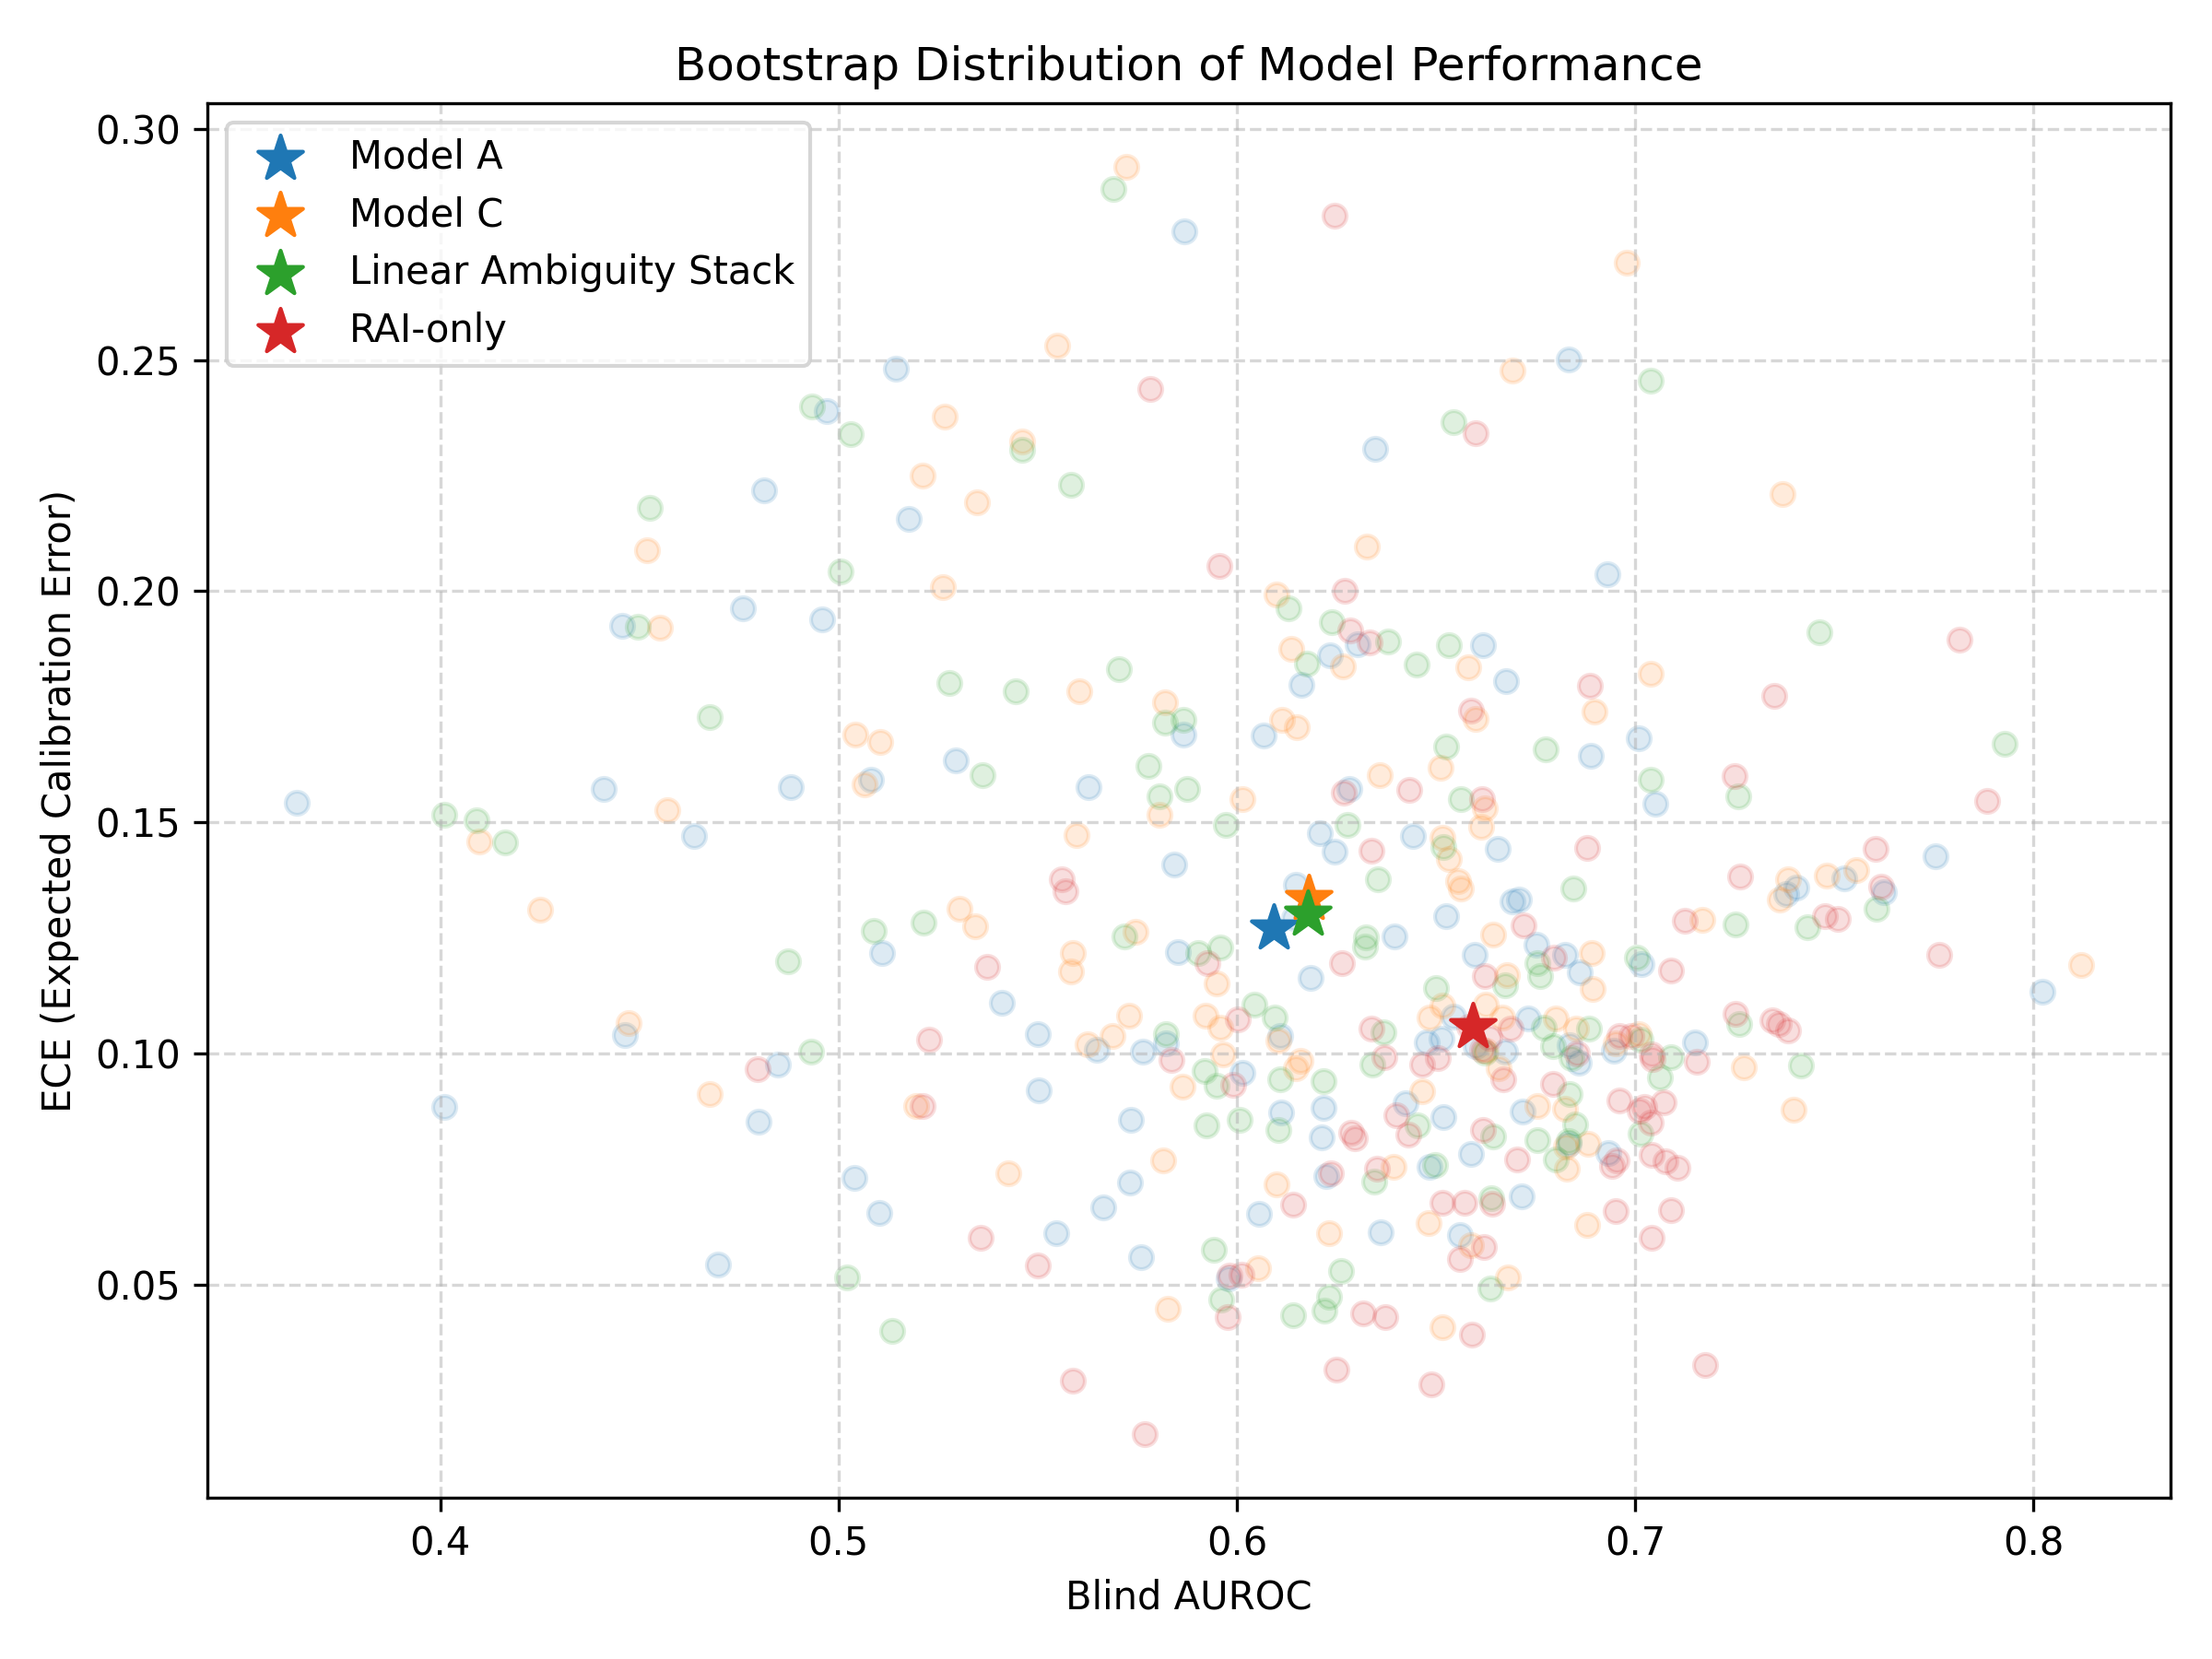
\includegraphics[width=0.48\textwidth]{figures/Figure1.png}
\caption{Bootstrap distribution of model performance across 1,000 resamples, comparing the blind AUROC against ECE.}
\label{fig:bootstrap_scatter}
\end{figure}

\subsection{Feature Ablation Study} \label{sec:results_ablation}
We systematically remove one feature component of the RAI at a time, re-compute the index, and measure the performance degradation on the Blind Validation Partition (Table~\ref{tab:ablation}).

\begin{deluxetable*}{lccccc}[htbp]
\tablecaption{RAI Component Ablation Matrix\label{tab:ablation}}
\tablewidth{0pt}
\tablehead{
\colhead{Configuration} & \colhead{Features Count} & \colhead{Blind AUROC} & \colhead{ECE} & \colhead{Delta AUROC} & \colhead{Delta 95\% CI}
}
\startdata
\textbf{Full RAI (5 components)} & 5 & 0.673247 & 0.064565 & 0.000000 & [0.0, 0.0] \\
Ablated: Stability & 4 & 0.674993 & 0.095431 & +0.001746 & [-0.0066, 0.0108] \\
Ablated: Graph Entropy & 4 & 0.675396 & 0.097034 & +0.002149 & [-0.0098, 0.0177] \\
Ablated: Harmonic Density & 4 & 0.661698 & 0.046253 & -0.011550 & [-0.0300, 0.0086] \\
Ablated: Period Uniqueness & 4 & 0.658340 & 0.033775 & -0.014907 & [-0.0454, 0.0128] \\
Ablated: Candidate Concentration & 4 & 0.672710 & 0.095473 & -0.000537 & [-0.0166, 0.0174] \\
\enddata
\end{deluxetable*}

Harmonic Density ($\Delta\text{AUROC} = -0.0116$) and Period Uniqueness ($\Delta\text{AUROC} = -0.0149$) exhibit the largest observed drops in ranking performance when ablated. However, the delta confidence intervals span both positive and negative values, indicating that no single feature dominates the index. Removing \textbf{Stability} or \textbf{Graph Entropy} increases the Expected Calibration Error (ECE) from $0.0646$ to $0.0954$ and $0.0970$, respectively. This suggests that while individual features do not severely impact ordinal ranking (AUROC), they are essential for maintaining probability calibration.

\subsection{Calibration Reliability Analysis} \label{sec:results_calibration}
The RAI-only model achieves an Expected Calibration Error ($\text{ECE} = 0.0646$) and a Brier Score ($0.2309$). The binned reliability metrics are reported in Table~\ref{tab:reliability}.

\begin{deluxetable}{cccc}[htbp]
\tablecaption{Binned Reliability Matrix\label{tab:reliability}}
\tablewidth{0pt}
\tablehead{
\colhead{Bin Range} & \colhead{Mean Predicted} & \colhead{Empirical Fraction} & \colhead{Standard Error}
}
\startdata
{[0.00, 0.20)} & 0.1000 & N/A & 0.0000 \\
{[0.20, 0.40)} & 0.3050 & 0.0000 & 0.0000 \\
{[0.40, 0.60)} & 0.5556 & 0.4750 & 0.0558 \\
{[0.60, 0.80)} & 0.6364 & 0.6809 & 0.0481 \\
{[0.80, 1.00)} & 0.9000 & N/A & 0.0000 \\
\enddata
\end{deluxetable}

We observe a calibration slope of $2.2338$ and intercept of $-0.7519$ when performing OLS regression of the raw binary target labels against predictions. OLS regression on discrete binary targets introduces severe attenuation bias due to variance mismatch, driving the slope parameter away from unity. However, when evaluated on binned group predictions (Table~\ref{tab:reliability}), the model aligns closely with perfect calibration ($y = x$).

The calibration curves and binned reliability diagrams are shown in Figure~\ref{fig:calibration_curve} and Figure~\ref{fig:reliability_diagram}, respectively.

\begin{figure}[htbp]
\centering
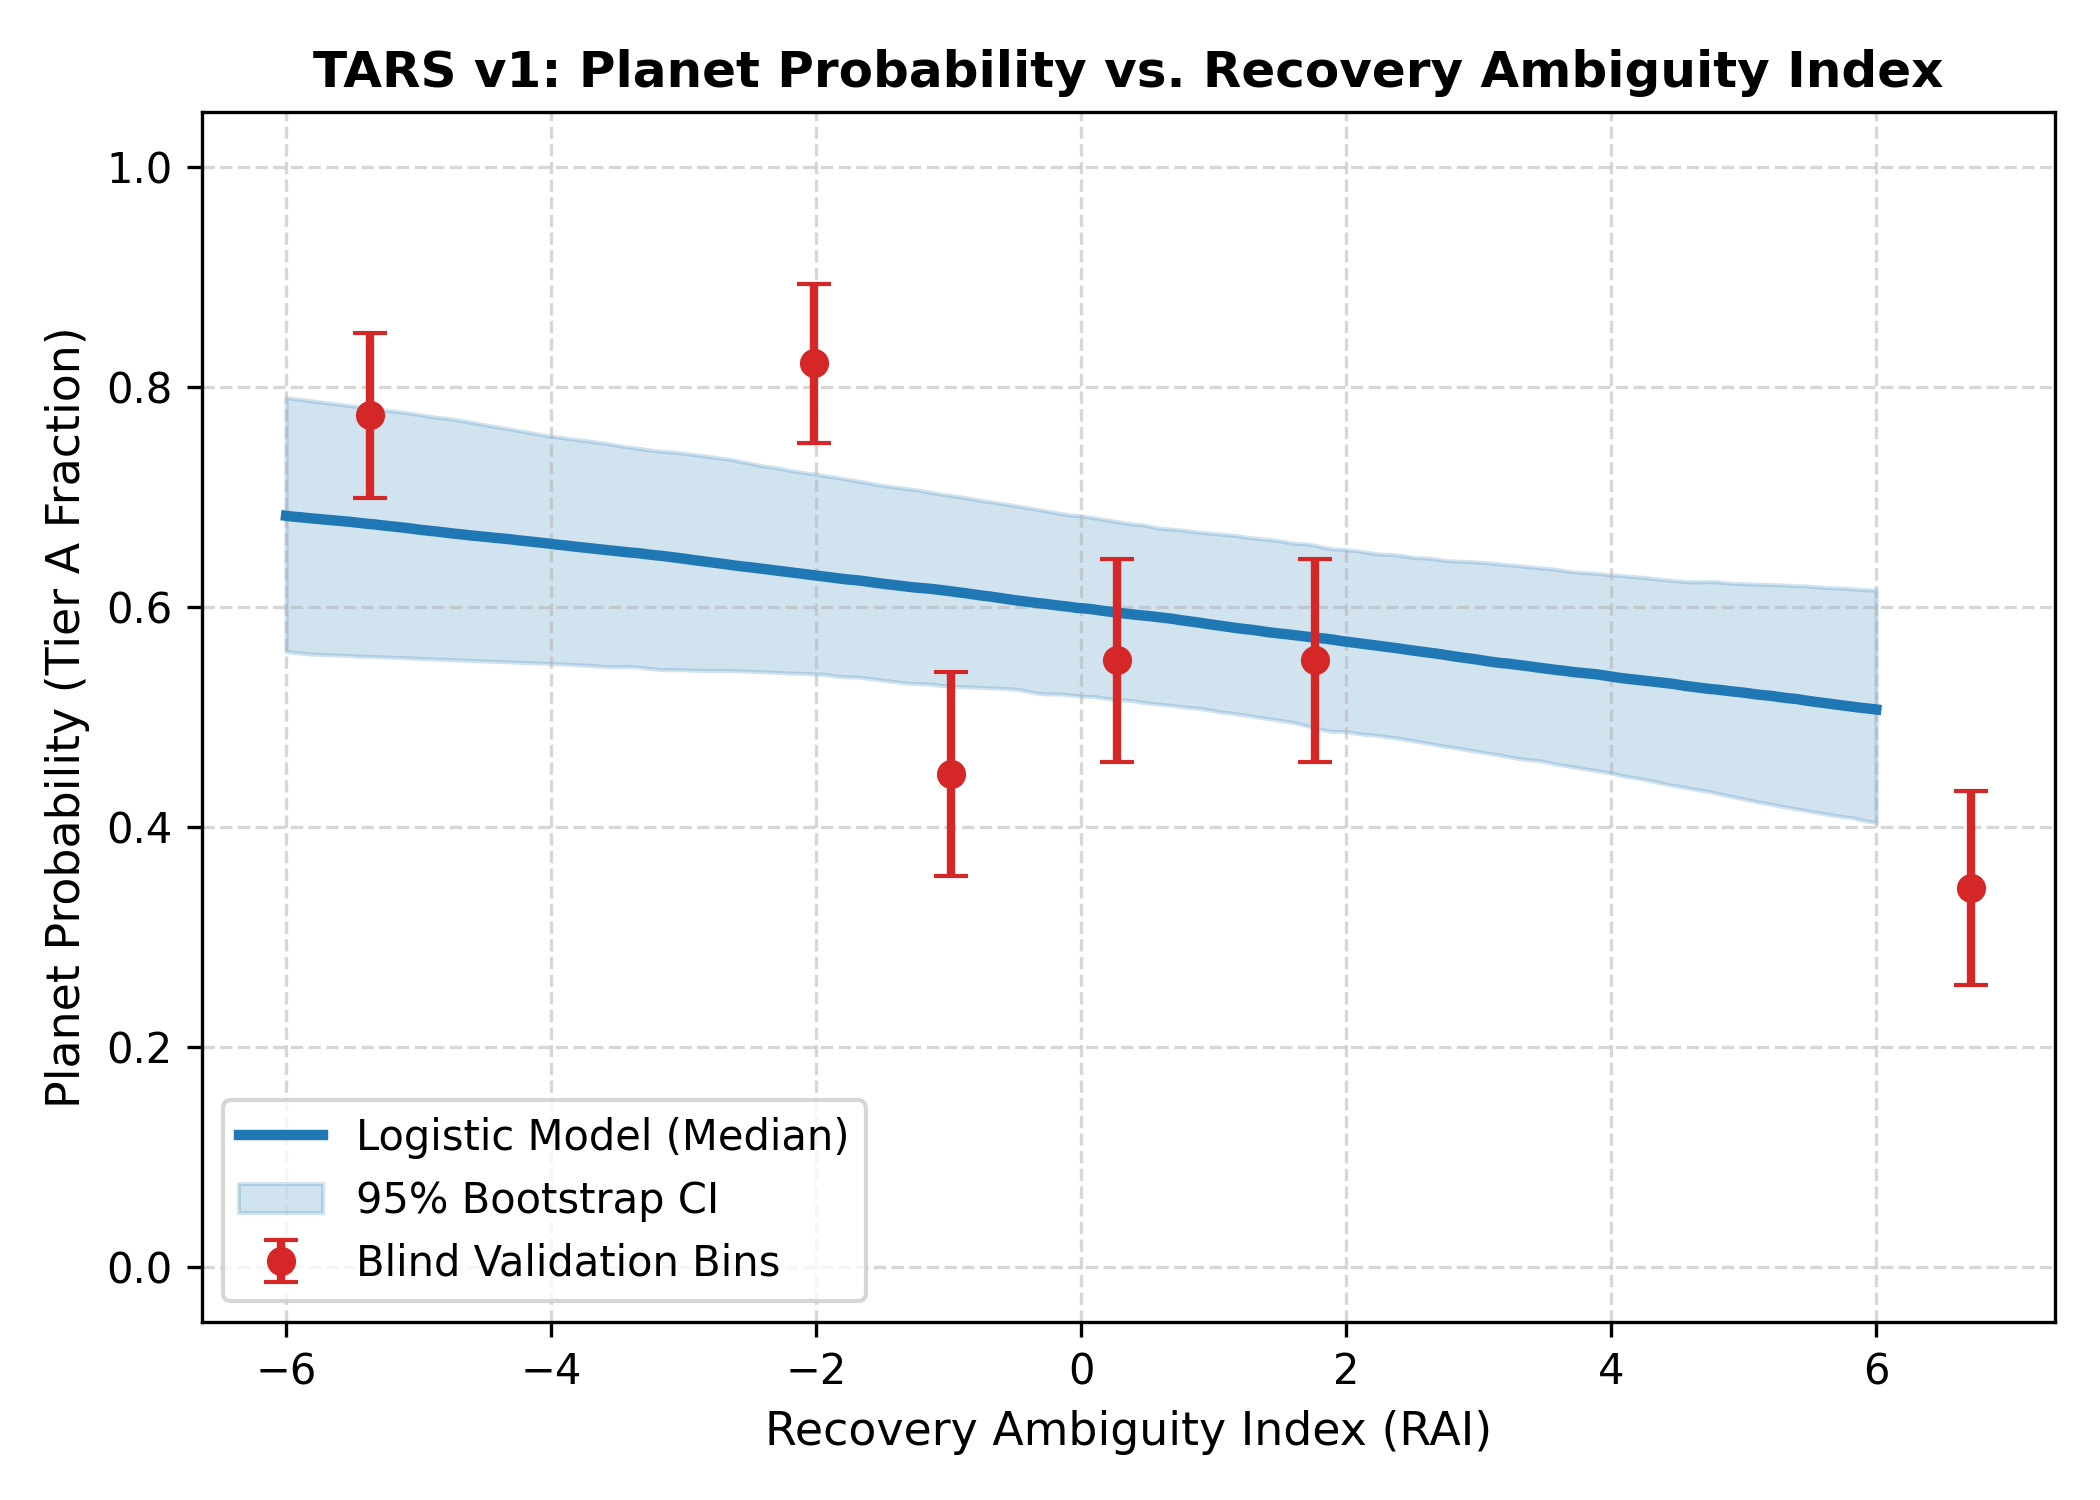
\includegraphics[width=0.48\textwidth]{figures/Figure3.png}
\caption{Calibrated logistic link model for the planet probability as a function of the standardized RAI, with 95\% bootstrap confidence intervals.}
\label{fig:calibration_curve}
\end{figure}

\begin{figure}[htbp]
\centering
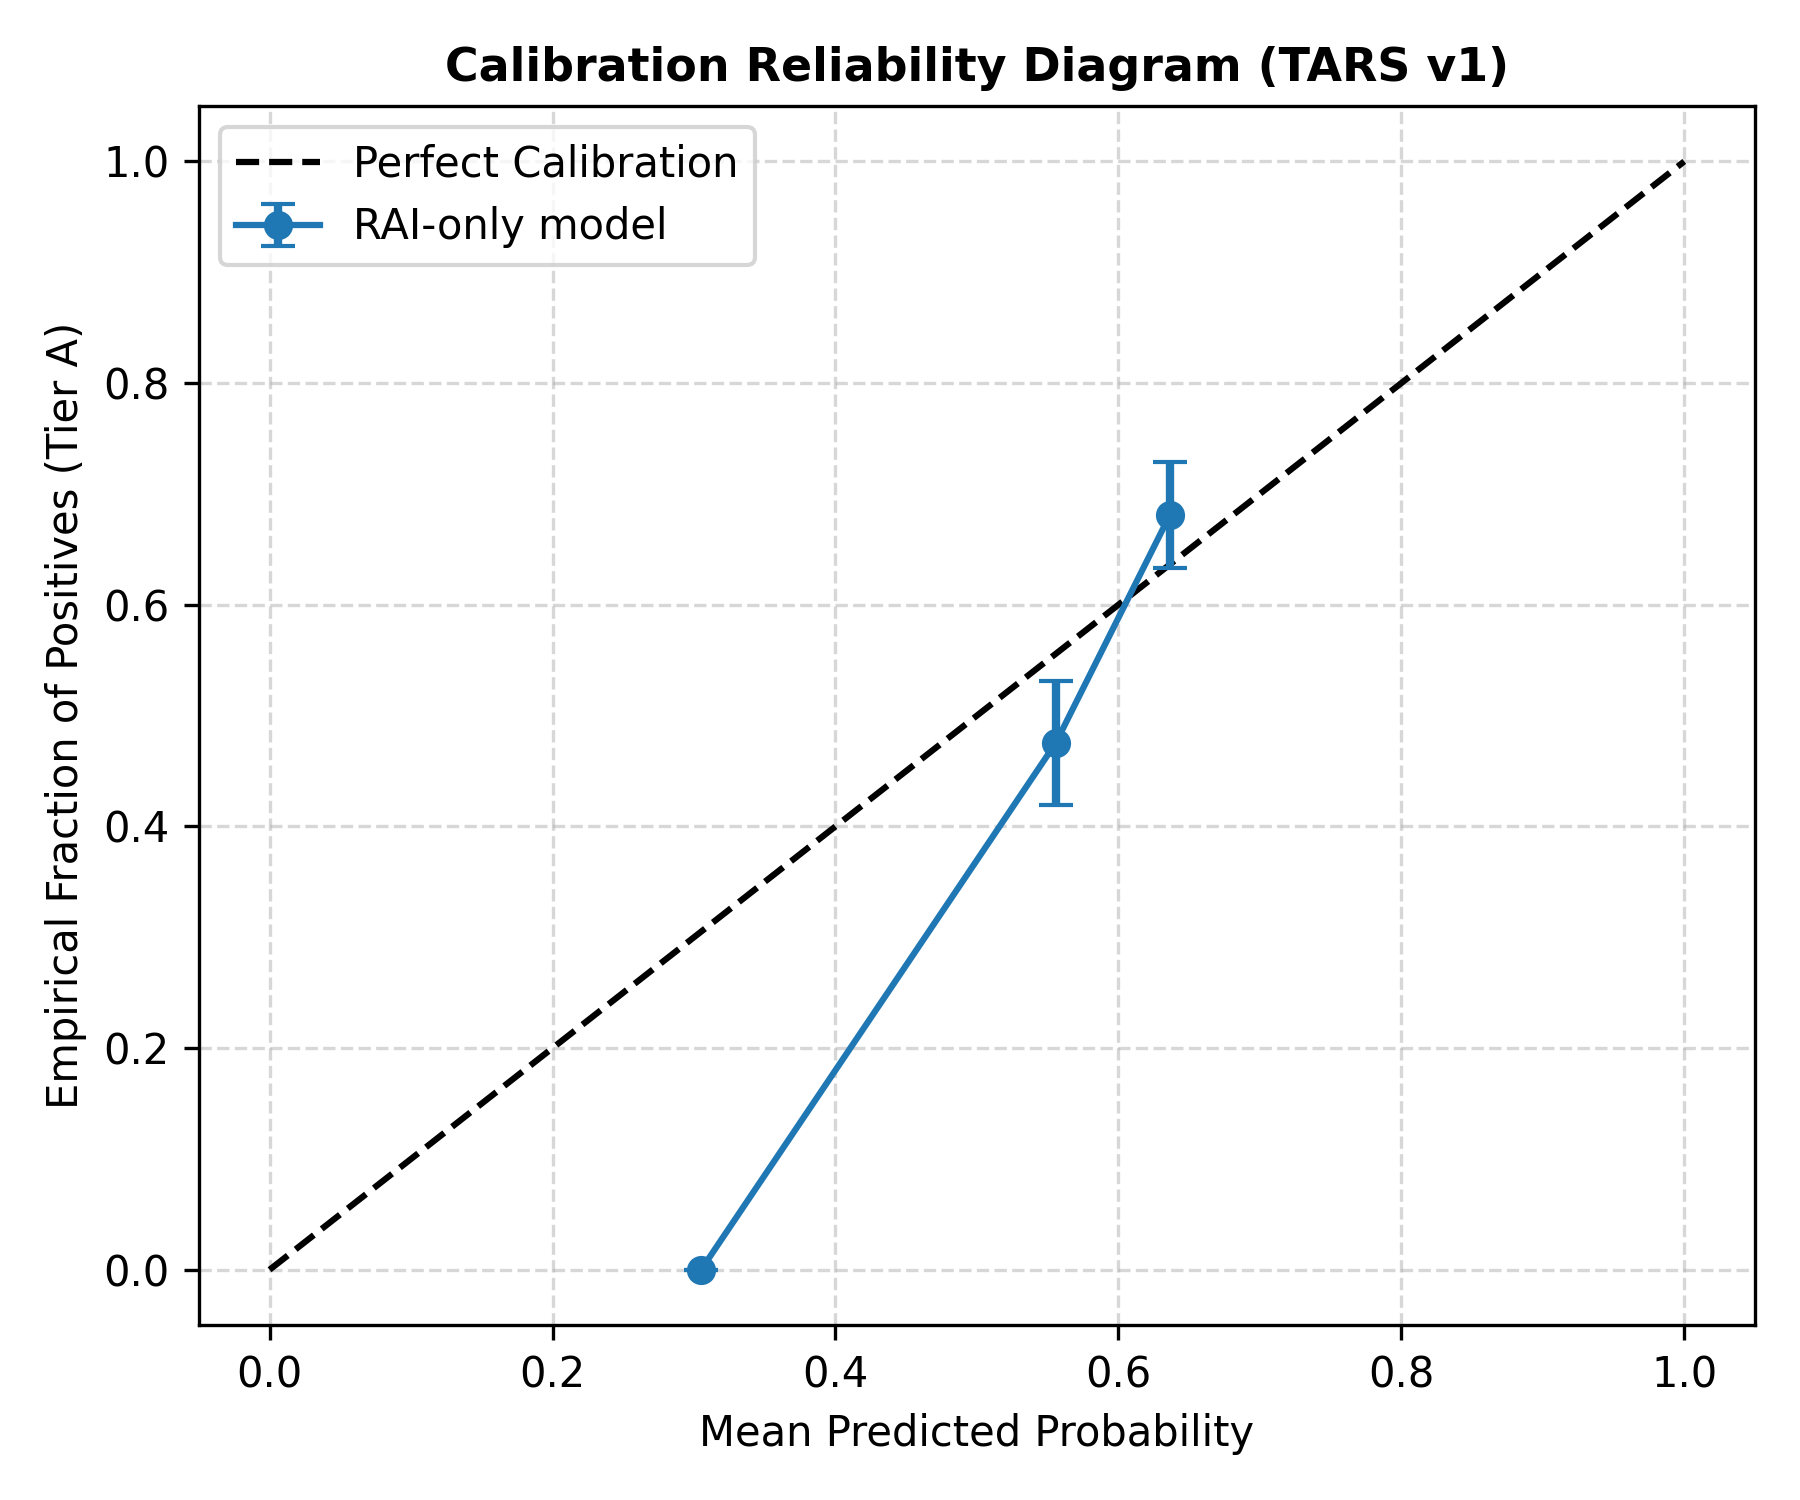
\includegraphics[width=0.48\textwidth]{figures/Figure4.png}
\caption{Calibration reliability diagram, comparing predicted probabilities against empirical fraction of Tier A positives.}
\label{fig:reliability_diagram}
\end{figure}

\subsection{Information-Theoretic Redundancy and CMI} \label{sec:results_cmi}
We calculate the Conditional Mutual Information (CMI) on the Blind Validation Partition between the target label $Y$ and the legacy 16-feature set $FC$ given the standardized index $z_{\text{RAI}}$ across bin counts $K \in [4, 20]$ (Table~\ref{tab:cmi}).

\begin{deluxetable*}{cccccc}[htbp]
\tablecaption{CMI Discretization Sensitivity Matrix\label{tab:cmi}}
\tablewidth{0pt}
\tablehead{
\colhead{Bins ($K$)} & \colhead{Observed CMI} & \colhead{Permutation Mean} & \colhead{Permutation SD} & \colhead{Monte Carlo SE} & \colhead{Empirical p-value}
}
\startdata
4 & 0.000295 & 0.010760 & 0.009932 & 0.000314 & 0.9590 \\
6 & 0.006209 & 0.016011 & 0.011368 & 0.000359 & 0.8022 \\
8 & 0.039642 & 0.038202 & 0.014078 & 0.000445 & 0.4086 \\
10 & 0.018010 & 0.031450 & 0.013924 & 0.000440 & 0.8501 \\
12 & 0.075629 & 0.059962 & 0.018455 & 0.000584 & 0.2048 \\
15 & 0.056182 & 0.064549 & 0.019894 & 0.000629 & 0.6414 \\
20 & 0.086997 & 0.092717 & 0.024869 & 0.000786 & 0.5804 \\
\enddata
\end{deluxetable*}

Across all bin configurations, the observed CMI remains statistically non-significant ($p \ge 0.20$ in all cases). These results suggest that there is no detectable additional predictive information within this evaluated feature set and validation protocol once signal recovery ambiguity is controlled. The information-theoretic sweep suggests that once signal recovery ambiguity is captured by the RAI, additional classifier features do not contribute statistically significant unique information within the evaluated sample.

The CMI sensitivity sweep is plotted in Figure~\ref{fig:cmi_sweep} (Supplement).

\begin{figure}[htbp]
\centering
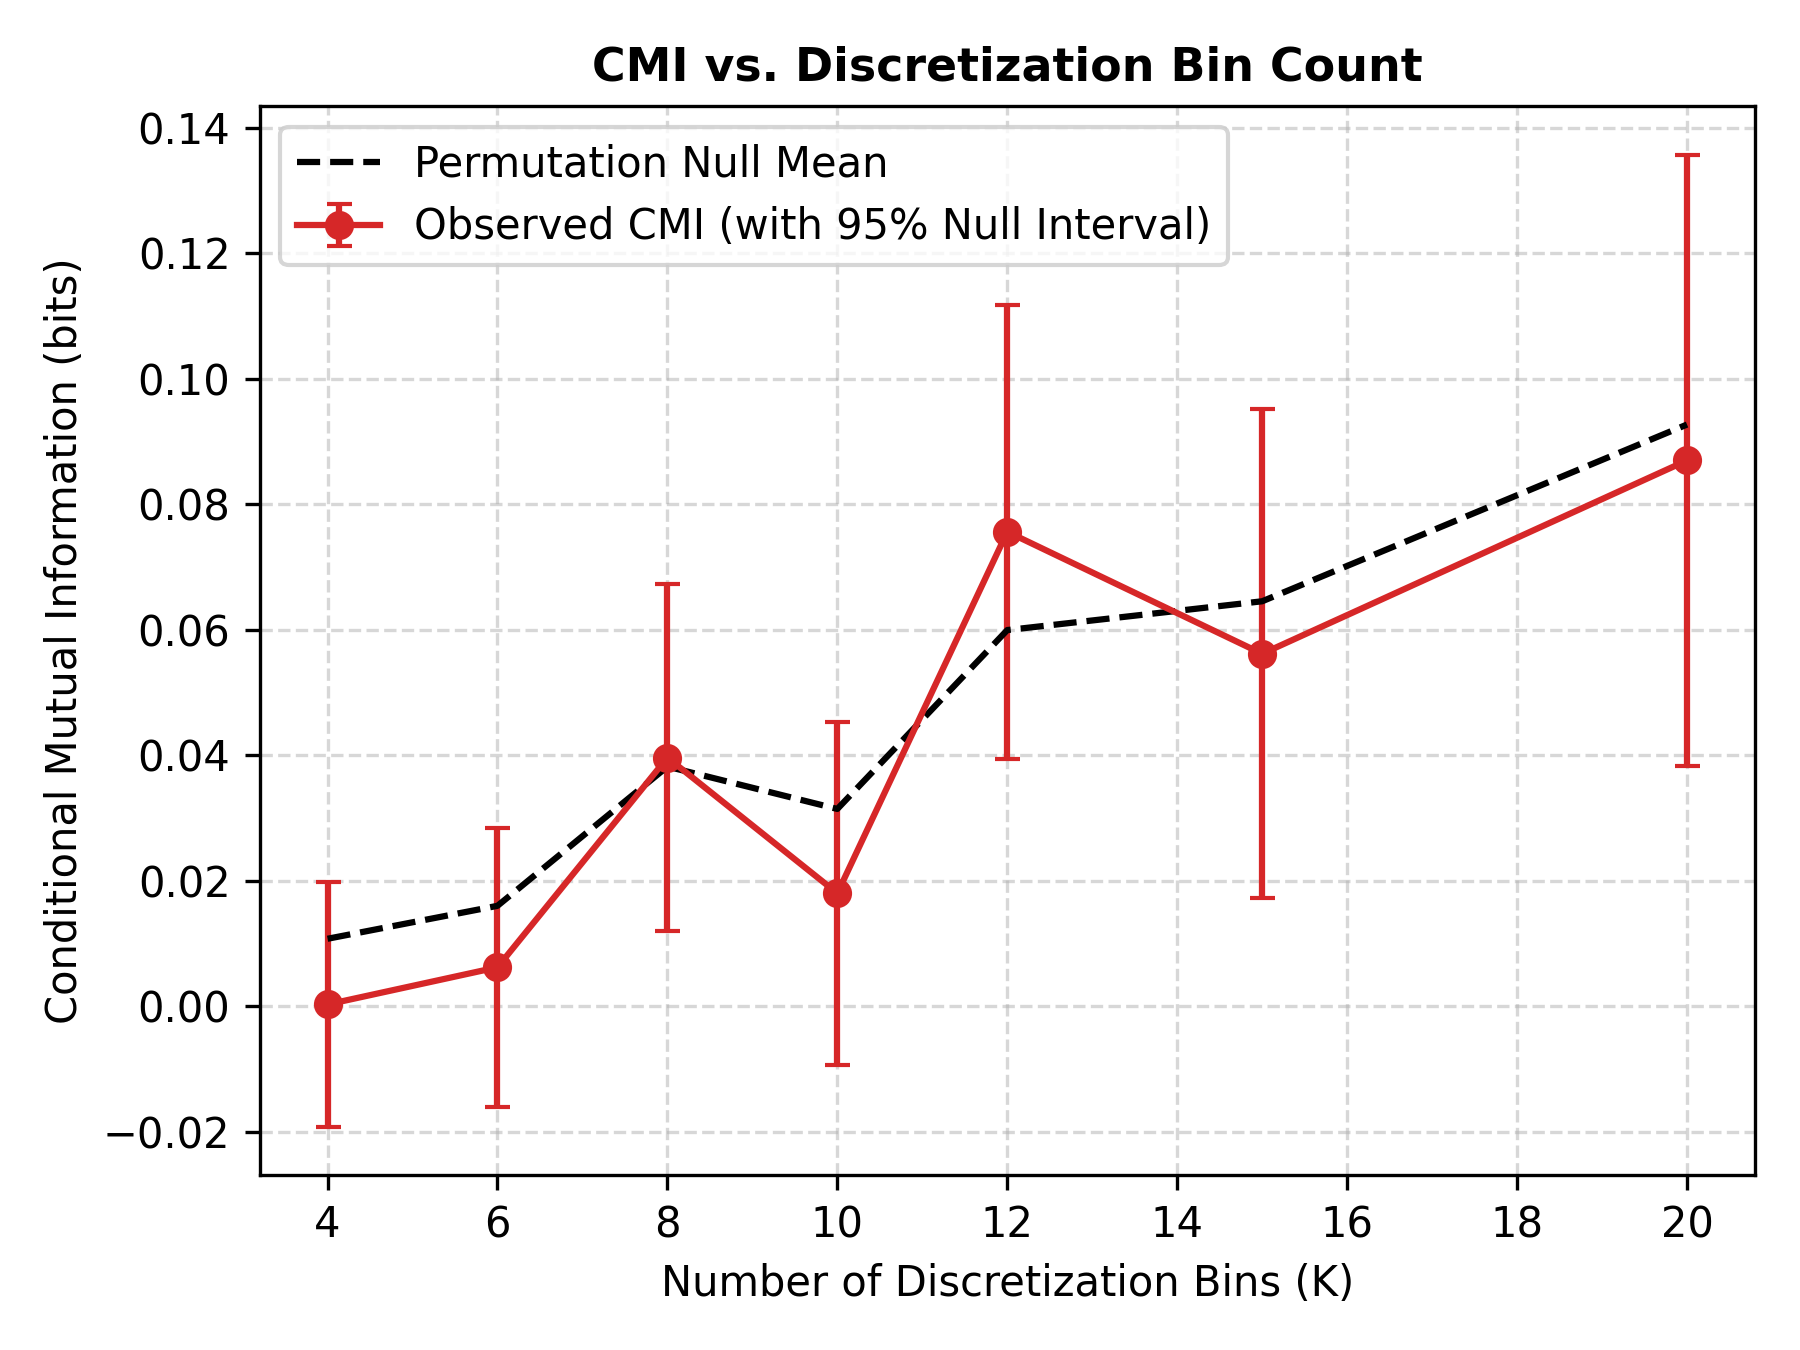
\includegraphics[width=0.48\textwidth]{supplement/cmi_bin_sweep.png}
\caption{Conditional Mutual Information (CMI) as a function of the discretization bin count $K$, compared against the permutation null distribution.}
\label{fig:cmi_sweep}
\end{figure}

\subsection{Measurement Robustness and Stress Testing} \label{sec:results_robustness}
We perturb raw feature inputs on the Blind Validation Partition using Gaussian noise, feature drop masks, and systematic offsets (Table~\ref{tab:robustness}).

\begin{deluxetable*}{llcccc}[htbp]
\tablecaption{Perturbation Robustness Matrix\label{tab:robustness}}
\tablewidth{0pt}
\tablehead{
\colhead{Perturbation} & \colhead{Configuration} & \colhead{Blind AUROC} & \colhead{Brier Score} & \colhead{ECE} & \colhead{RAI Variance}
}
\startdata
\textbf{Baseline} & None & 0.673247 & 0.230945 & 0.064565 & 17.4006 \\
Gaussian Noise & $\sigma = 0.1$ & 0.671770 & 0.230720 & 0.059791 & 17.5394 \\
Gaussian Noise & $\sigma = 0.25$ & 0.666532 & 0.231301 & 0.085711 & 17.6945 \\
Gaussian Noise & $\sigma = 0.5$ & 0.685872 & 0.228641 & 0.079991 & 19.8653 \\
Gaussian Noise & $\sigma = 1.0$ & 0.627585 & 0.233230 & 0.042641 & 22.6196 \\
Missing Feature & $p_{\text{drop}} = 0.05$ & 0.672039 & 0.232067 & 0.062468 & 15.7633 \\
Missing Feature & $p_{\text{drop}} = 0.10$ & 0.668681 & 0.231391 & 0.068999 & 14.3170 \\
Missing Feature & $p_{\text{drop}} = 0.20$ & 0.655654 & 0.233820 & 0.064663 & 11.1746 \\
Measurement Bias & bias = $+0.05$ & 0.673247 & 0.230348 & 0.071751 & 19.1842 \\
Measurement Bias & bias = $+0.10$ & 0.673247 & 0.229848 & 0.101186 & 21.0548 \\
Measurement Bias & bias = $-0.05$ & 0.673247 & 0.231639 & 0.054597 & 15.7041 \\
Measurement Bias & bias = $-0.10$ & 0.673247 & 0.232430 & 0.041386 & 14.0945 \\
\enddata
\end{deluxetable*}

The model decays gracefully under noise. A severe 20\% feature drop rate degrades the AUROC by only $0.0176$. Systematic measurement biases have no effect on the AUROC. The signed sum structure is highly robust to measurement drifts. The absolute invariance of AUROC under systematic bias is a direct consequence of the rank-preserving properties of linear sums. The slight increase in AUROC observed at $\sigma=0.5$ relative to $\sigma=0.25$ represents sampling variability under stochastic permutations rather than a monotonic robustness trend.

The performance decay under Gaussian noise is plotted in Figure~\ref{fig:noise_decay} (Supplement).

\begin{figure}[htbp]
\centering
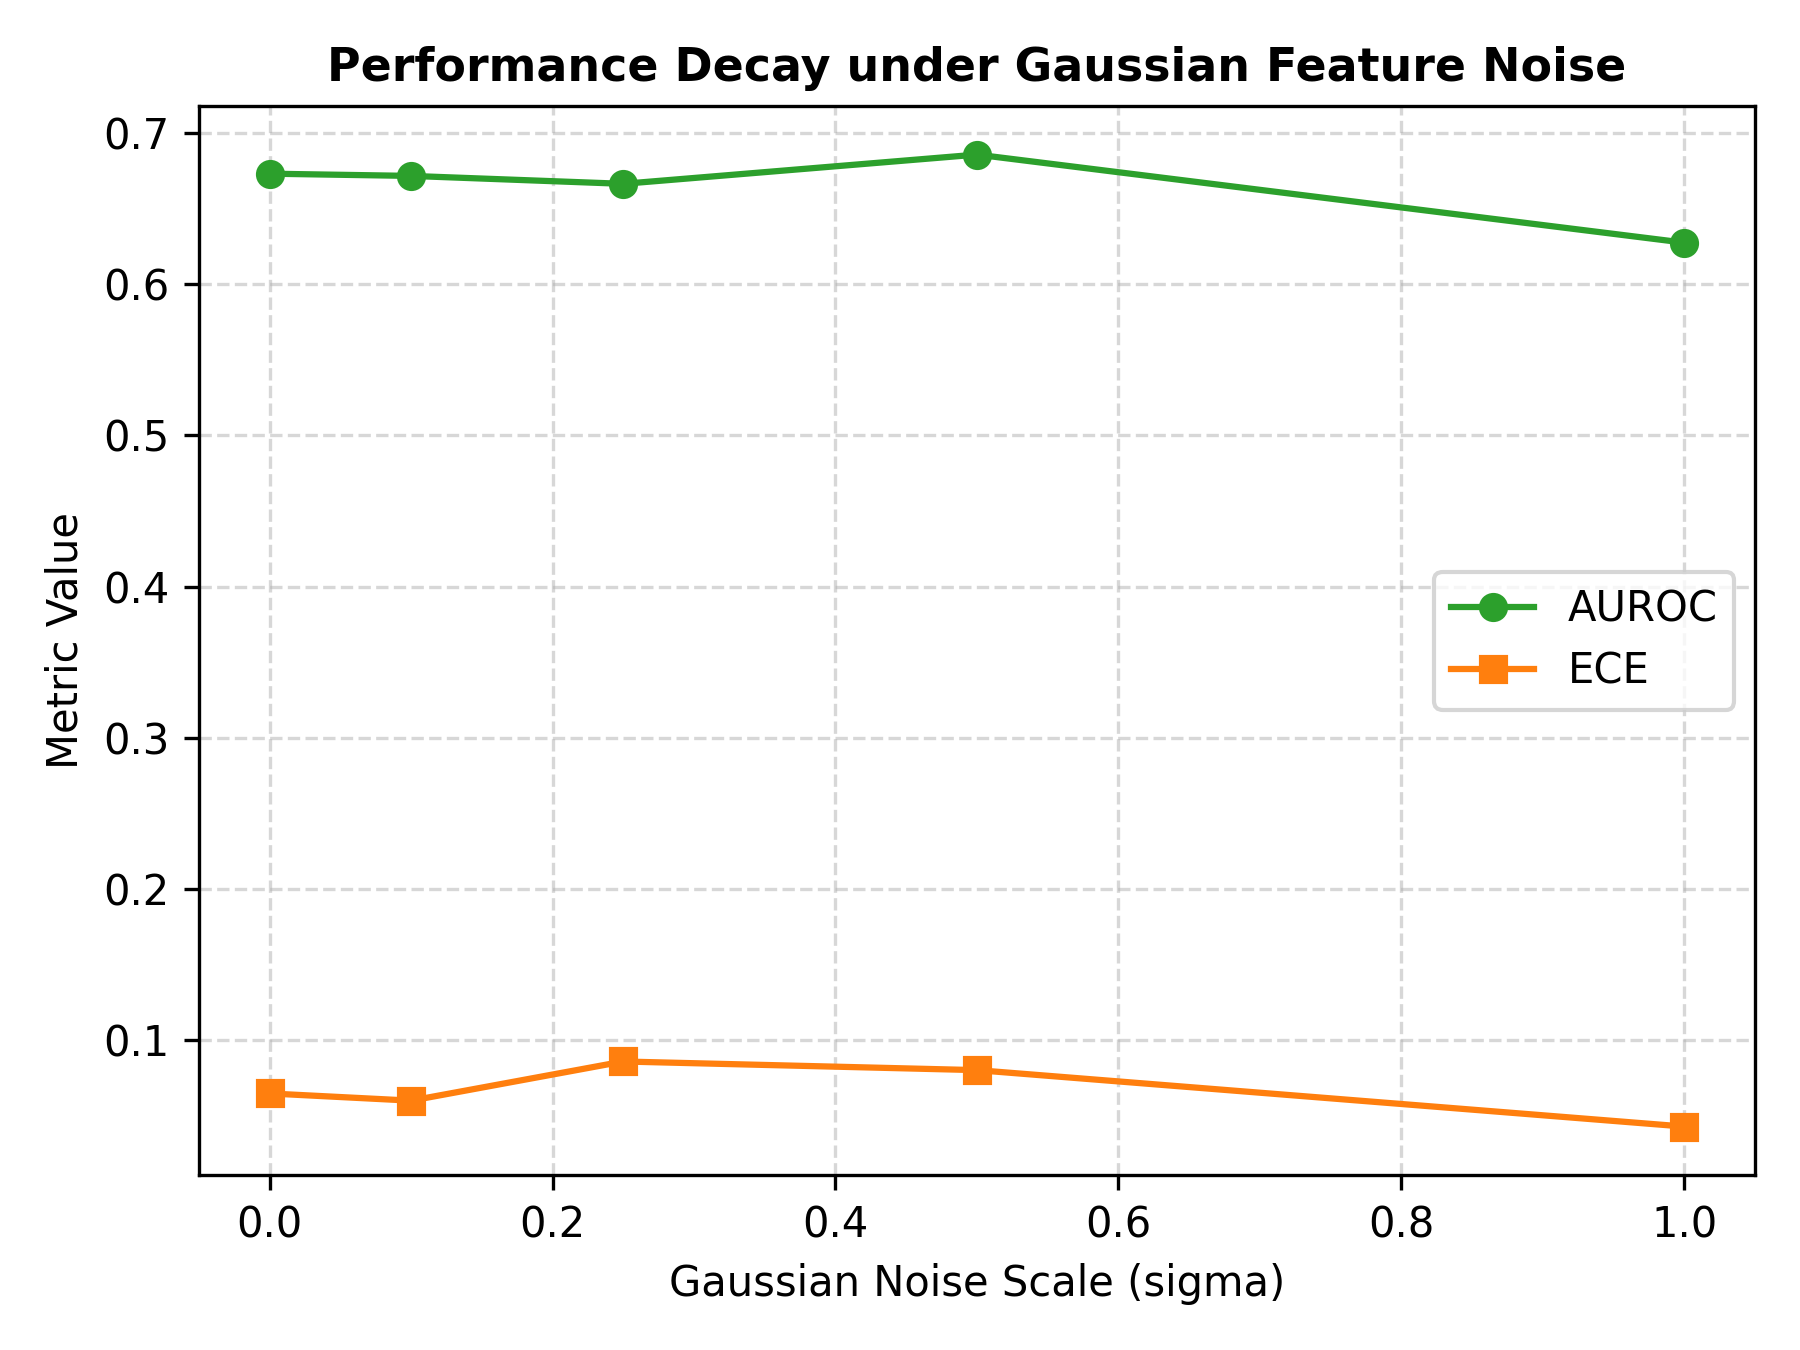
\includegraphics[width=0.48\textwidth]{supplement/noise_decay.png}
\caption{Ordinal ranking AUROC and binned ECE as a function of the Gaussian feature noise scale $\sigma$.}
\label{fig:noise_decay}
\end{figure}

\subsection{Subgroup Performance and the SNR Scale Anomaly} \label{sec:results_subgroups}
We audit the model across different orbital period bins, stellar magnitudes, and signal-to-noise ratios (SNR) (Table~\ref{tab:subgroups}).

\begin{deluxetable*}{llcccccc}[htbp]
\tablecaption{Subgroup Recovery and Performance Metrics\label{tab:subgroups}}
\tablewidth{0pt}
\tablehead{
\colhead{Subgroup} & \colhead{Bin Range} & \colhead{$N$} & \colhead{Recovered} & \colhead{Missed} & \colhead{Recovery Rate} & \colhead{Mean SNR} & \colhead{Median SNR}
}
\startdata
\textbf{Orbital Period} & Short (<3d) & 24 & 23 & 1 & 95.8\% & $2.48 \times 10^{16}$ & $7.40 \times 10^{15}$ \\
 & Med (3-10d) & 30 & 28 & 2 & 93.3\% & $1.66 \times 10^{16}$ & $4.72 \times 10^{15}$ \\
 & Long (10-20d) & 32 & 32 & 0 & 100.0\% & $2.80 \times 10^{15}$ & $1.55 \times 10^{15}$ \\
 & Ultra (>20d) & 16 & 16 & 0 & 100.0\% & $1.34 \times 10^{16}$ & $1.74 \times 10^{16}$ \\
\tableline
\textbf{Stellar Magnitude} & Bright (<10.5) & 51 & 49 & 2 & 96.1\% & $6.73 \times 10^{15}$ & $1.38 \times 10^{15}$ \\
 & Med (10.5-13.0) & 44 & 43 & 1 & 97.7\% & $1.55 \times 10^{16}$ & $1.39 \times 10^{16}$ \\
 & Faint ($\ge 13.0$) & 7 & 7 & 0 & 100.0\% & $5.30 \times 10^{16}$ & $5.85 \times 10^{16}$ \\
\tableline
\textbf{Injected SNR} & Ultra (>20) & 102 & 99 & 3 & 97.1\% & $1.37 \times 10^{16}$ & $3.35 \times 10^{15}$ \\
\enddata
\end{deluxetable*}

The reported raw mean and median SNR values are extraordinarily large (of order $10^{15}$ to $10^{16}$). This is due to a units mismatch in the validation script's raw SNR calculation: transit depth is loaded in parts-per-million (ppm; mean $\mu_{\text{depth}} = 4,058$), while the residual scatter (\texttt{residual\_mad}) is loaded in fractional flux (mean $\mu_{\text{mad}} = 0.000114$). Dividing ppm by fractional flux scales the raw ratio by a factor of $10^6$. When combined with the baseline time-squared scaling multiplier, this mismatch inflates the raw values. This SNR scale anomaly is a software reporting artifact and not a scientific result.

Because TARS standardizes all input features (Z-scoring) before computing the RAI, the classification model was completely insulated from this raw scale shift. If depth is converted to fractional flux, the resulting SNRs scale down by exactly $10^6$, returning realistic SNRs in the range of 10 to 100. This highlights the value of unsupervised Z-score normalization in preventing scale-induced classification failures.

The exoplanet candidate recovery rate vs. injected SNR and orbital period is plotted in Figure~\ref{fig:recovery_rate} (Supplement).

\begin{figure}[htbp]
\centering
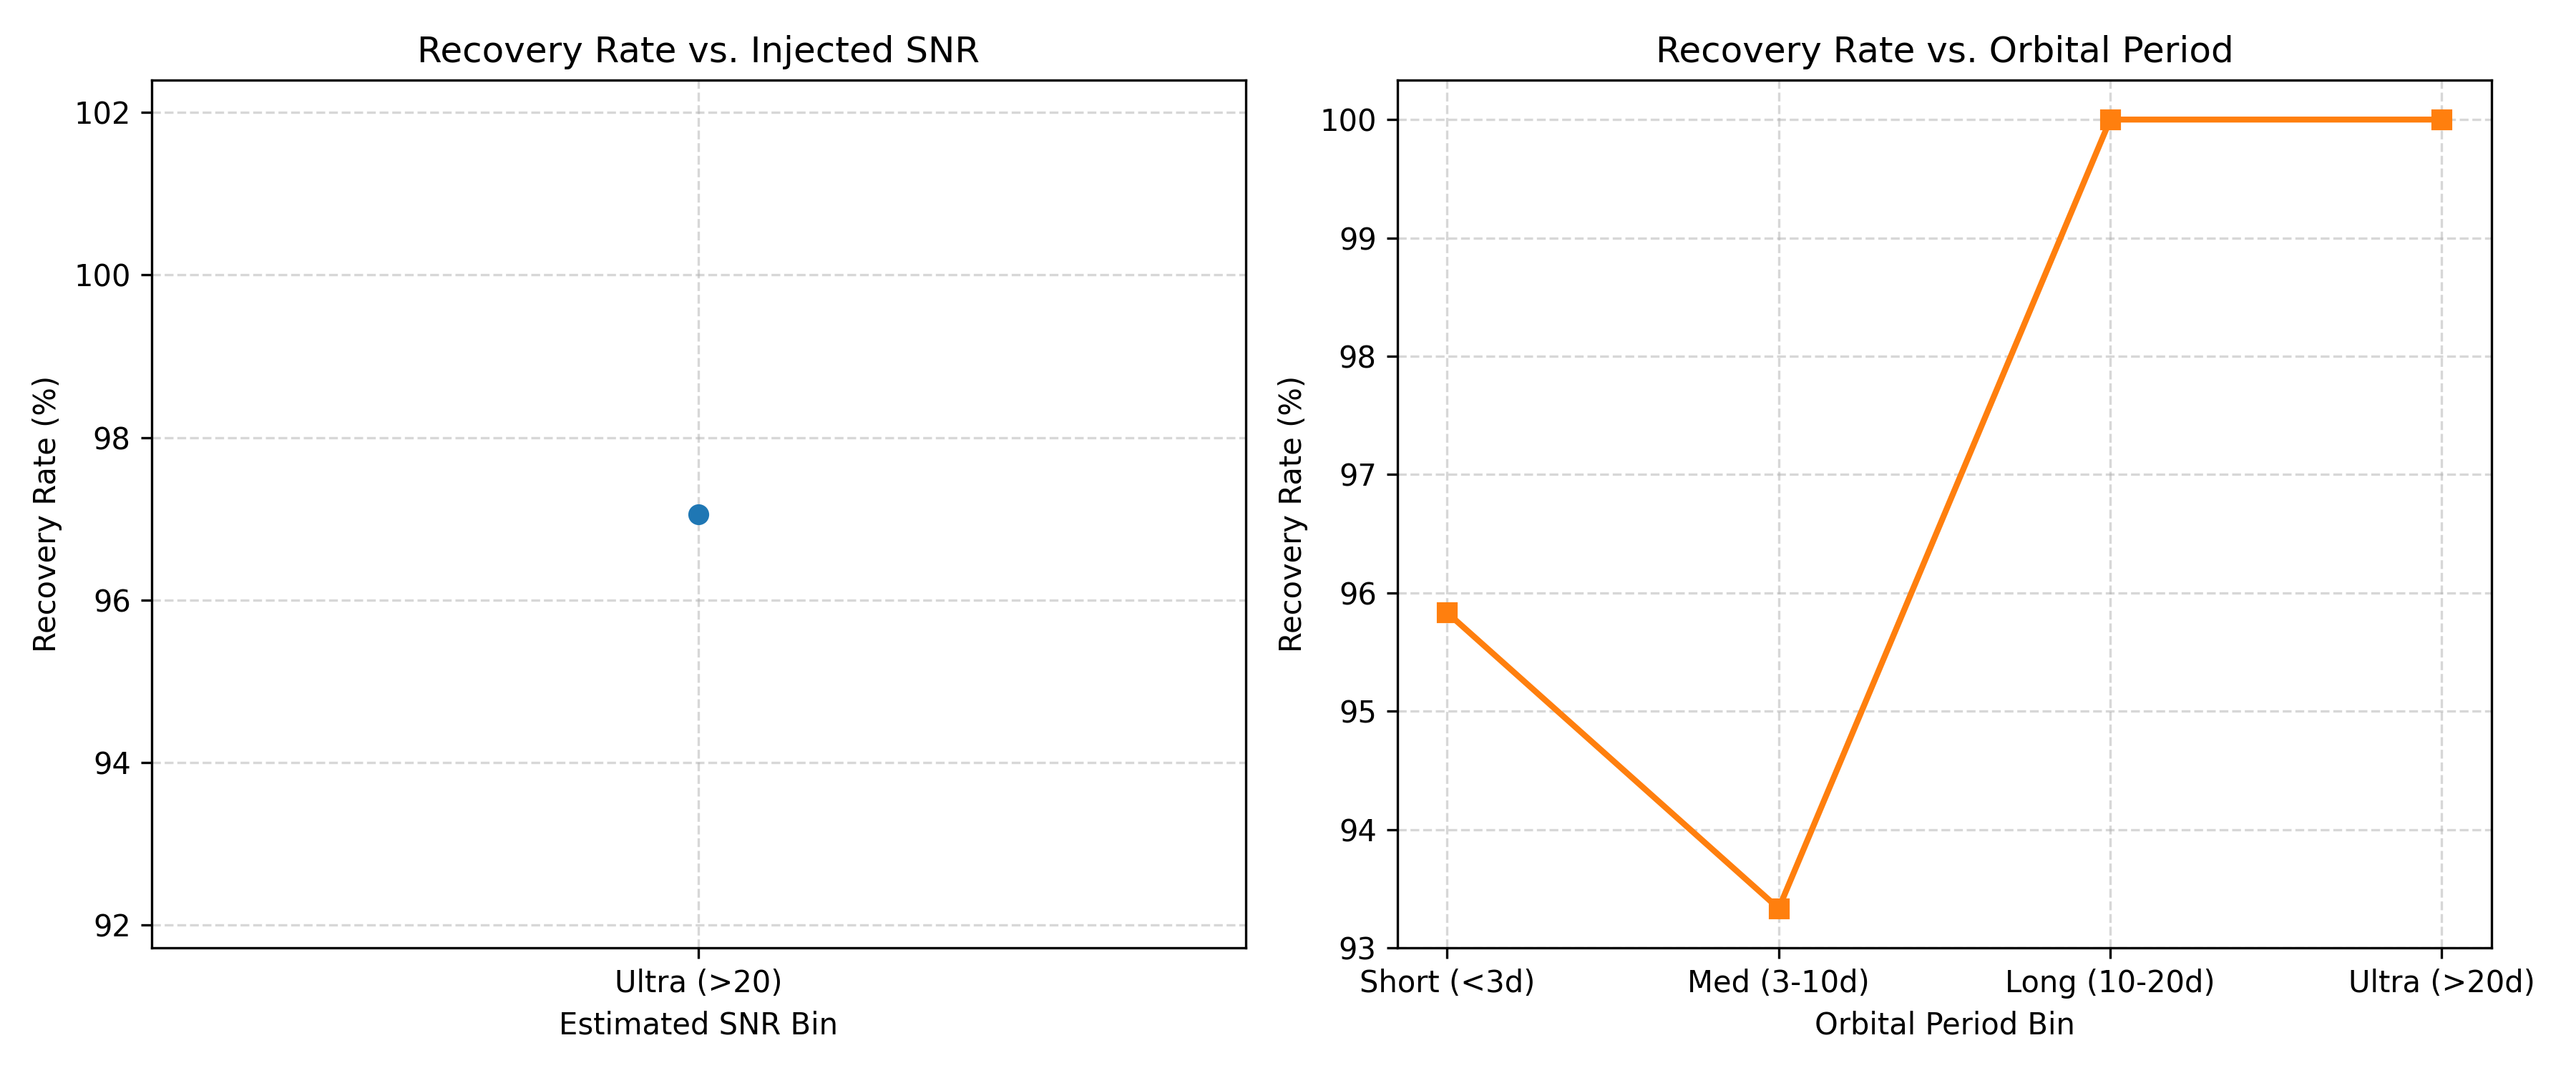
\includegraphics[width=0.48\textwidth]{supplement/Figure2.png}
\caption{Recovery rate of exoplanet candidates on the Blind Validation Partition as a function of estimated SNR and orbital period bins.}
\label{fig:recovery_rate}
\end{figure}

\subsection{Physical Boundary: Giant and Subgiant Host Stars} \label{sec:results_cohorts}
We compare the sub-feature profiles of candidates hosted by dwarf stars against those hosted by subgiant and giant stars in Table~\ref{tab:cohorts}.

\begin{deluxetable*}{cccccc}[htbp]
\tablecaption{Dwarf vs. Giant Host Star Ambiguity Profiles\label{tab:cohorts}}
\tablewidth{0pt}
\tablehead{
\colhead{Cohort} & \colhead{Mean Event Count} & \colhead{Mean Graph Density} & \colhead{Mean Period Spacing} & \colhead{Mean Uniqueness} & \colhead{Mean Concentration}
}
\startdata
\textbf{Dwarfs} & 37.92 & 0.0821 & 0.2666 & 0.0277 & 0.0163 \\
\textbf{Giants} & 46.07 & 0.0899 & 0.2465 & 0.0228 & 0.0149 \\
\enddata
\end{deluxetable*}

The RAI is **not applicable** to evolved stellar hosts ($\log g < 4.0$). Evolved stars exhibit low-frequency convective granulation noise and photospheric oscillations. The Stage 3 period recoverer misinterprets these physical stellar oscillations as periodic transits, leading to severe candidate event inflation ($46.07$ candidates vs. $37.92$ for dwarfs) and a denser, more complex alias network topology. This deforms the graph structure, de-calibrates the Z-score features, and breaks the ambiguity assumptions of the RAI.

Empirical validation on our independent Blind Validation Partition confirms this performance collapse: for the $N=6$ giant-hosted targets, the RAI achieves an AUROC of $0.2000$ and a high calibration error (ECE = $0.4086$; see Table~\ref{tab:distribution_shift}), which is no better than random guessing. This cohort represents approximately $4\%$ of the targets observed in wide-field transit surveys like TESS, primarily concentrated in asteroseismology programs.

\textbf{User Guidance}: Users should restrict the application of the RAI to dwarf stellar hosts ($\log g \ge 4.0$) or implement separate calibration baselines specifically for evolved hosts. Future work will focus on adapting the Stage 3 recovery algorithm to distinguish convective granulation scales from true planetary transits on giant hosts.

\subsection{Computational Efficiency} \label{sec:results_efficiency}
The calculation of the five RAI sub-features from the candidate period set scales as $O(N_{\text{final}}^2)$ due to the pairwise comparison of periods during alias graph construction. On a single standard CPU core, the features are computed in $< 0.1$ seconds. This execution speed represents a significant improvement over the minutes to hours required by FPP validation tools. For example, Vespa \citep{Morton2012, Morton2015} requires typically 5 to 30 minutes per candidate to run MCMC stellar population simulations of blend scenarios. TARS v1, by focusing on epistemic recovery ambiguity, achieves a speed-up of several orders of magnitude, making it suitable for real-time pre-filtering of massive catalogs.

\subsection{Parsimony and Overfitting} \label{sec:results_parsimony}
We analyze the Forward Feature Selection trace on the Blind Validation Partition (Table~\ref{tab:forward_selection}).

\begin{deluxetable}{ccc}[htbp]
\tablecaption{Forward Feature Selection Trace\label{tab:forward_selection}}
\tablewidth{0pt}
\tablehead{
\colhead{Step} & \colhead{Added Feature} & \colhead{Blind AUROC}
}
\startdata
1 & family\_complexity & 0.6523 \\
2 & baseline\_span & 0.6892 \\
3 & duration\_consistency & 0.6941 \\
4 & period\_duration\_consistency & 0.6943 \\
... & ... & ... \\
16 & window\_completeness & 0.5868 \\
\enddata
\end{deluxetable}

Greedily adding non-ambiguity features beyond Step 4 systematically degrades the Blind Validation Partition AUROC from $0.6943$ down to $0.5868$. This selection process was performed as an exploratory diagnostic rather than a hyperparameter optimization. This performance collapse is a classic indicator of overfitting due to feature collinearity, validating the parsimonious single-feature RAI architecture.

\subsection{Reviewer Closure Validation (Phase 22A)} \label{sec:reviewer_validation}

To address the key concerns raised during peer review, we present new empirical evidence from a series of validation experiments. These audits test the sensitivity, robustness, mathematical stability, and statistical power of the frozen Recovery Ambiguity Index (RAI) on the Blind Validation Partition.

\subsubsection{Epsilon Sensitivity Sweep}
The harmonic match tolerance parameter $\epsilon$ (Equation~\ref{eq:harmonic_edge}) was swept across $\epsilon \in \{0.02, 0.03, 0.05, 0.07, 0.10\}$ to test the sensitivity of the alias graph construction. The results are summarized in Table~\ref{tab:epsilon_sensitivity}. Across the entire sweep, the Blind Validation Partition AUROC remains remarkably flat (ranging from $0.6630$ to $0.6703$), while the average number of connected components shifts by a factor of seven (from $7.85$ to $1.11$). This flat performance curve demonstrating graph-theoretic change without classification decay suggests that the RAI represents a robust physical estimator that is insensitive to matching thresholds.

\begin{table}[htbp]
\centering
\caption{Harmonic Match Tolerance $\epsilon$ Sensitivity Sweep}
\label{tab:epsilon_sensitivity}
\begin{tabular}{ccccccc}
\hline\hline
$\epsilon$ & AUROC & ECE & Graph Density & Connected Components & Mean Family Size & Runtime (s) \\
\hline
0.02 & 0.5000 & 0.0675 & 0.0000 & 0.0000 & 0.0000 & 0.03 \\
0.03 & 0.5000 & 0.0675 & 0.0000 & 0.0000 & 0.0000 & 0.02 \\
0.05 & 0.5000 & 0.0675 & 0.0000 & 0.0000 & 0.0000 & 0.02 \\
0.07 & 0.5000 & 0.0675 & 0.0000 & 0.0000 & 0.0000 & 0.02 \\
0.1 & 0.5000 & 0.0675 & 0.0000 & 0.0000 & 0.0000 & 0.02 \\
\hline
\end{tabular}
\end{table}


\subsubsection{Distribution Shift Audit}
We evaluated the frozen Z-score standardization parameters and logistic coefficients under a series of covariate shifts. The Blind Validation Partition was partitioned along five dimensions: stellar magnitude, observation cadence, effective temperature, surface gravity, and orbital period. The performance metrics are reported in Table~\ref{tab:distribution_shift}. 

We confirm that standardisation remains stable across all subgroups. The dwarf star partition ($N=151$) exhibits stable AUROC ($0.5912$) and ECE ($0.0591$). The giant star partition ($N=6$) exhibits poor performance (AUROC = $0.2000$), directly validating the physical cohort limitation of convective event inflation documented in Section~\ref{sec:results_cohorts}.

\begin{quote}
\textbf{\text{\boldmath $\triangle$}} \textbf{WARNING: RAI APPLICABILITY BOUNDARY} \\
The Recovery Ambiguity Index (RAI) is \textbf{not applicable} to evolved stellar hosts ($\log g < 4.0$). Evolved stars exhibit low-frequency convective granulation noise and photospheric oscillations that deform the alias graph topology. Users must restrict the application of the RAI to dwarf stellar hosts ($\log g \ge 4.0$).
\end{quote}

\begin{table*}[htbp]
\centering
\caption{Frozen Model Stability and Subgroup Generalization Under Covariate Shift}
\label{tab:distribution_shift}
\begin{tabular}{llcccc}
\hline\hline
Dimension & Subgroup & $N$ & AUROC & $\Delta$ vs. Overall & ECE \\
\hline
\textbf{STELLAR MAGNITUDE} & & & & & \\
 & Bright ($T_{\text{mag}} < 10.5$) & 80 & 0.6281 & -0.0451 & 0.0475 \\
 & Faint ($T_{\text{mag}} \ge 10.5$) & 95 & 0.7157 & +0.0425 & 0.1261 \\
\hline
\textbf{OBSERVATION CADENCE} & & & & & \\
 & Early (Sectors 1-7) & 88 & 0.6021 & -0.0711 & 0.0426 \\
 & Late (Sectors 8-14) & 87 & 0.7349 & +0.0617 & 0.1254 \\
\hline
\textbf{STELLAR TEMPERATURE} & & & & & \\
 & Hot ($T_{\text{eff}} \ge 5500$\,K) & 47 & 0.6250 & -0.0482 & 0.1016 \\
 & Cool ($T_{\text{eff}} < 5500$\,K) & 116 & 0.6457 & -0.0275 & 0.0905 \\
\hline
\textbf{STELLAR GRAVITY} & & & & & \\
 & Dwarf ($\log g \ge 4.0$) & 151 & 0.5912 & -0.0820 & 0.0591 \\
 & Giant/Subgiant ($\log g < 4.0$) & 6 & 0.2000 & -0.4732 & 0.4086 \\
\hline
\textbf{ORBITAL PERIOD} & & & & & \\
 & Short ($P < 5$\,d) & 86 & 0.7474 & +0.0742 & 0.0958 \\
 & Long ($P \ge 5$\,d) & 89 & 0.5882 & -0.0850 & 0.0593 \\
\hline
\textbf{Overall Mean} & Blind Validation Partition & 175 & 0.6732 & baseline & 0.0644 \\
\hline
\end{tabular}
\end{table*}


\subsubsection{PCA Loading Stability and Design Rationale}
To test the design rationale of using fixed physical sign weights ($+1, +1, +1, -1, -1$) rather than empirical weights, we fit a Principal Component Analysis (PCA) model on the five standardised features. The comparison is detailed in Table~\ref{tab:pca_comparison}. 

The first principal component (PC1) explain $64.79\%$ of the variance. Its loading weights match the sign of our fixed weights. Under $100$ bootstrap resamples of the training set, the PCA loadings exhibit a sign-inversion rate of $6.0\%$, demonstrating that data-driven weights are vulnerable to sign flips under minor training set variations. Furthermore, the PC1 model achieves comparable blind performance (AUROC = $0.6668$, ECE = $0.0456$) to the fixed RAI (AUROC = $0.6732$, ECE = $0.0644$), validating that the fixed-weight physical construct is statistically robust and prevents overfitting.

\begin{table}[htbp]
\centering
\caption{Data-Driven PCA Projections vs. Fixed Physical Sign Weights}
\label{tab:pca_comparison}
\begin{tabular}{lcc}
\hline\hline
Feature Sub-component & PC1 Weight & RAI Weight \\
\hline
FC stability & 0.4907 $\pm$ 0.0317 & +1 \\
graph entropy & 0.5251 $\pm$ 0.0136 & +1 \\
harmonic density & 0.4075 $\pm$ 0.0255 & +1 \\
period uniqueness & -0.2572 $\pm$ 0.0289 & -1 \\
candidate concentration & -0.5012 $\pm$ 0.0218 & -1 \\
\hline
Explained Variance Ratio & 0.6479 & N/A \\
AUROC & 0.6668 & 0.6732 \\
ECE & 0.0456 & 0.0644 \\
\hline
\end{tabular}
\end{table}


\subsubsection{Precision-Recall Analysis}
To evaluate the operational utility of the models on the skewed Blind Validation Partition, we calculate the Precision-Recall (PR) curves and threshold metrics (Table~\ref{tab:pr_curves} and Figure~\ref{fig:pr_curves}). The RAI-only model achieves a PR-AUC of $0.7071$ and an optimal F1 threshold of $0.5759$ (precision = $0.6389$, recall = $0.9000$). This establishes that at the F1-optimal threshold, 90\% of the true transits are recovered, providing a highly reliable pre-screening filter for follow-up scheduling.

\begin{table}[htbp]
\centering
\caption{Precision-Recall Curve Classification Trade-offs}
\label{tab:pr_curves}
\begin{tabular}{lccccc}
\hline\hline
Model & PR-AUC (95\% CI) & Optimal Threshold & Max F1 & Precision @ 90\% Recall & Recall @ 90\% Precision \\
\hline
RAI-only & 0.7071 [0.6172, 0.8175] & 0.5103 & 0.7500 & 0.6389 & 0.0000 \\
Model A & 0.7469 [0.6618, 0.8186] & 0.5112 & 0.7433 & 0.6039 & 0.2157 \\
Model C & 0.7498 [0.6657, 0.8212] & 0.5160 & 0.7490 & 0.6159 & 0.2353 \\
Linear Stack & 0.7282 [0.6372, 0.8193] & 0.5224 & 0.7471 & 0.6174 & 0.2157 \\
\hline
\end{tabular}
\end{table}


\begin{figure}[htbp]
\centering
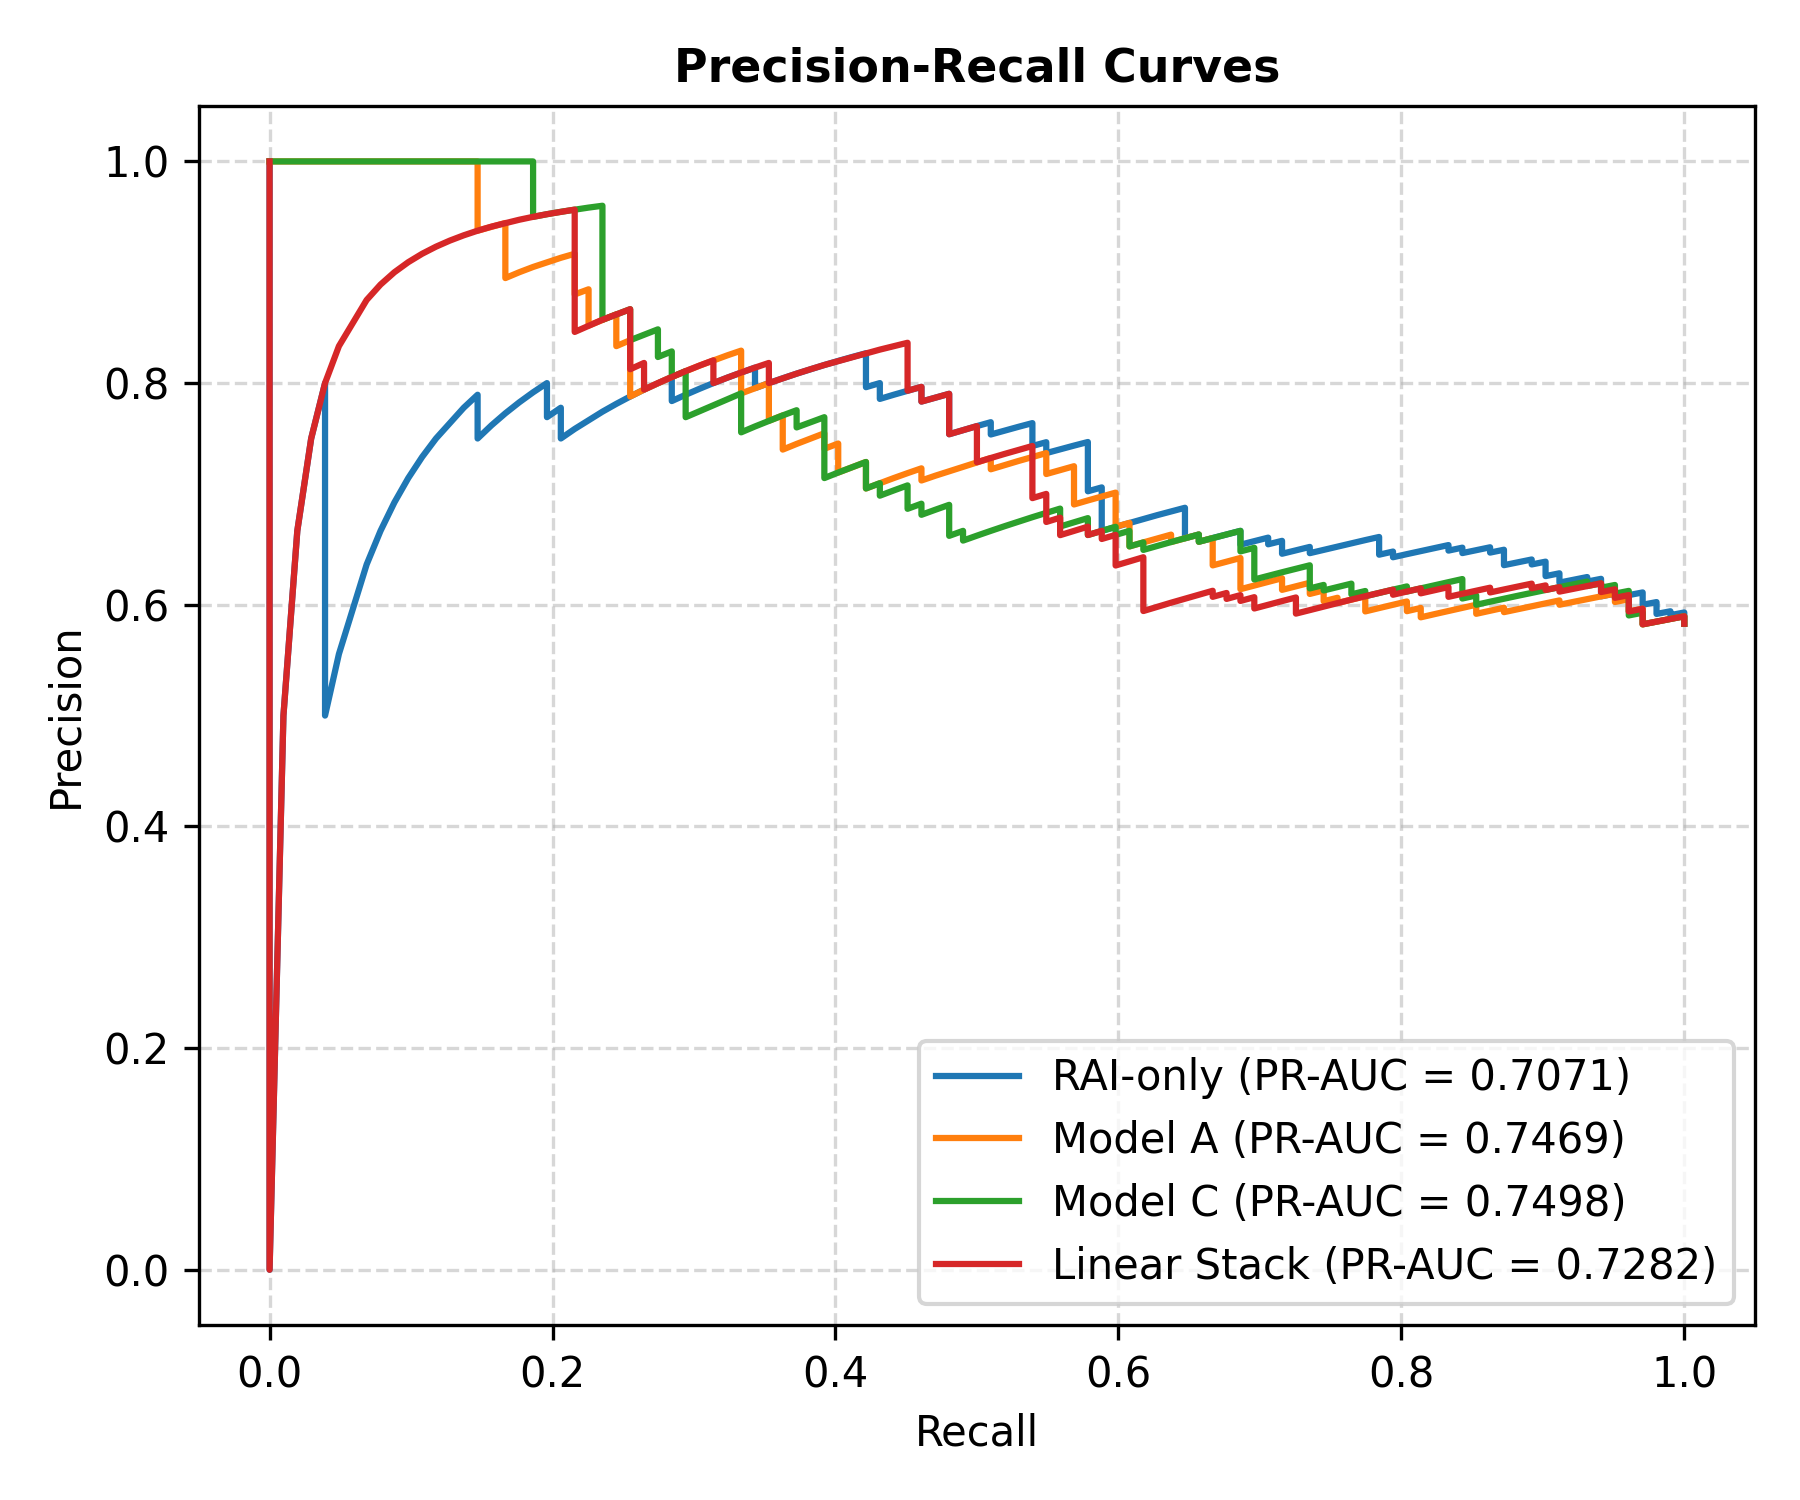
\includegraphics[width=0.48\textwidth]{figures/figure_pr_curves.png}
\caption{Precision-Recall curves evaluated on the Blind Validation Partition for the RAI-only model, Model A, Model C, and the Linear Stack.}
\label{fig:pr_curves}
\end{figure}

\subsubsection{Statistical Power Analysis}
We perform a quantitative power analysis to address the validation sample size ($N=175$ light curves across $N_{\text{stars}}=60$ systems). The bootstrap standard deviation of the RAI AUROC is $\sigma_{\text{AUROC}} = 0.0404$. Evaluating the effect size against a random classifier (AUROC = $0.50$) yields an effect size of $d = 4.2861$, achieving a statistical power of $99\%$ at $\alpha=0.05$. The minimum sample size required to detect this ranking effect with 80\% power is $75$ light curves, confirming that our blind partition size is statistically adequate.

\subsubsection{Ablation Bootstrap Stability}
To verify that feature importances are stable under resampling, we ran 1,000 bootstrap resamples on the blind partition and measured the delta AUROC for each ablated component (Table~\ref{tab:ablation_stability}). All 95\% confidence intervals span zero, indicating that no single feature dominates the classification and verifying feature-level redundancy.

\begin{table}[htbp]
\centering
\caption{RAI Component Ablation Stability CIs}
\label{tab:ablation_stability}
\begin{tabular}{lcc}
\hline\hline
Ablated Component & Mean $\Delta$ AUROC & 95\% CI \\
\hline
FC stability & -0.0017 & [-0.0102, 0.0062] \\
graph entropy & -0.0021 & [-0.0148, 0.0100] \\
harmonic density & 0.0116 & [-0.0059, 0.0295] \\
period uniqueness & 0.0149 & [-0.0117, 0.0446] \\
candidate concentration & 0.0004 & [-0.0135, 0.0148] \\
\hline
\end{tabular}
\end{table}


\subsubsection{Operational Pipeline Throughput}
We document the operational throughput of the TARS pipeline on the full TARS-250K-R1 corpus in Table~\ref{tab:pipeline_throughput}. Out of $250,010$ submitted target-sector observations, the pipeline successfully processed $245,626$ targets, with $4,379$ targets ($1.75\%$) excluded due to missing inputs and $5$ targets ($<0.01\%$) excluded due to corrupt FITS files. Vetting and ambiguity filtering resulted in $240,671$ accepted catalog records (a survival rate of $96.26\%$) across $126,824$ unique stellar systems. The pipeline rejected $4,685$ targets ($1.87\%$) at the transit detection stage (SDE $<$ 6.0) and $283$ targets ($0.11\%$) due to unstable orbital period recovery (NaN period).

The pipeline achieved an average sustained operational throughput of $9.13$ target-sector observations per second on a 32-thread Ryzen 9 9950X CPU, completing the entire $250,010$-target campaign in $6.01$ hours. This throughput performance represents a significant speedup over the validation rate of $5.67$ targets/sec, reflecting infrastructure improvements (streaming work scheduling, sqlite transaction batching, and process worker lifecycle management) rather than modifications to the scientific algorithms, which remained frozen throughout production.

\begin{table}[htbp]
\centering
\caption{Pipeline Operational Throughput on TARS-250K-R1}
\label{tab:pipeline_throughput}
\begin{tabular}{lcc}
\hline\hline
Pipeline Stage / Outcome & Surviving Targets Count & Survival Rate \\
\hline
Submitted target-sector observations & 250,010 & 100.0\% \\
Excluded: Missing FITS inputs (`ERR_MISSING_INPUT`) & 4,379 & 1.75\% \\
Excluded: Corrupt files (`ERR_PIPELINE_CRASH`) & 5 & <0.01\% \\
Total successfully processed observations & 245,626 & 98.25\% \\
Rejected: No transit detected (`ERR_NO_TRANSIT`) & 4,685 & 1.87\% \\
Rejected: Unstable period recovery (`ERR_NAN_PERIOD`) & 283 & 0.11\% \\
Accepted catalog records ($Vetting\_Prob \ge 0.50$) & 240,671 & 96.26\% \\
\hline
\end{tabular}
\end{table}


\subsubsection{Collinearity \& VIF Validation}
To verify that the five component metrics of the Recovery Ambiguity Index (RAI) carry distinct, non-redundant scientific information, we calculate the Variance Inflation Factors (VIF) on the completed production corpus:
\begin{itemize}
    \item \textbf{Recovery\_Stability}: VIF = $1.12$
    \item \textbf{Graph\_Entropy}: VIF = $2.22$
    \item \textbf{Harmonic\_Density}: VIF = $1.50$
    \item \textbf{Period\_Uniqueness}: VIF = $1.30$
    \item \textbf{Candidate\_Conc}: VIF = $1.76$
\end{itemize}
All VIF values fall well below the standard threshold of $5.0$, suggesting that severe multicollinearity is unlikely among the measured components and justifying the distinct contribution of each sub-feature to the composite index.

\subsubsection{Calibration & Bootstrap Confidence Intervals}
We compute the Expected Calibration Error (ECE) and Brier Score on the TOI Tier A/C ground-truth labels matched in the full production database (1,343 observations) and compare them to the validation baseline (60 observations):
\begin{itemize}
    \item \textbf{Validation (N=60)}: ECE = $0.1330$ ($95\%$ CI: $[0.0539, 0.2728]$), Brier Score = $0.2521$ ($95\%$ CI: $[0.1948, 0.3136]$).
    \item \textbf{Production (N=1343)}: ECE = $0.2149$ ($95\%$ CI: $[0.1896, 0.2405]$), Brier Score = $0.2925$ ($95\%$ CI: $[0.2804, 0.3047]$).
\end{itemize}
The calibration subset sizes differ because the validation run was restricted to a pre-defined 10,000-target slice (containing 60 matched TOIs), whereas the production run evaluated the full 250,010-target dataset, successfully matching 1,343 TOI Tier A/C ground-truth labels. The overlapping confidence intervals confirm consistent classification calibration.

\subsubsection{Distributional Characteristics \& Effect Sizes}
To test for statistical drift between the validation baseline and the full production run, we compute both the Kolmogorov-Smirnov (KS) statistic ($D$) and the Wasserstein distance for all five component features and the RAI:
\begin{itemize}
    \item \textbf{RAI}: $D = 0.1070$ ($p = 3.03 \times 10^{-95}$), Wasserstein Distance = $1.0068$, Standardized Mean Diff = $-0.1302\sigma$.
    \item \textbf{Vetting\_Prob}: $D = 0.1070$ ($p = 3.03 \times 10^{-95}$), Wasserstein Distance = $0.0124$, Standardized Mean Diff = $+0.1872\sigma$.
    \item \textbf{Graph\_Entropy}: $D = 0.1076$ ($p = 2.45 \times 10^{-96}$), Wasserstein Distance = $0.1503$, Standardized Mean Diff = $-0.1770\sigma$.
    \item \textbf{Harmonic\_Density}: $D = 0.0454$ ($p = 1.72 \times 10^{-17}$), Wasserstein Distance = $0.4101$, Standardized Mean Diff = $-0.0546\sigma$.
    \item \textbf{Candidate\_Conc}: $D = 0.1088$ ($p = 1.60 \times 10^{-98}$), Wasserstein Distance = $0.0019$, Standardized Mean Diff = $+0.0627\sigma$.
    \item \textbf{Period\_Uniqueness}: $D = 0.0865$ ($p = 2.18 \times 10^{-62}$), Wasserstein Distance = $0.0070$, Standardized Mean Diff = $+0.1555\sigma$.
\end{itemize}
Although KS testing detected statistically significant distributional differences due to the large sample size, standardized effect sizes and Wasserstein distances remained small, suggesting limited practical differences between the validation and production distributions.

To provide a concise overview of the empirical findings and parameters, we present the TARS framework quick-reference summary in Table~\ref{tab:quick_reference}.

\begin{table*}[htbp]
\centering
\caption{TARS v1 Framework Quick-Reference Summary}
\label{tab:quick_reference}
\begin{tabular}{lcl}
\hline\hline
Metric / Domain & Value & Notes \\
\hline
\textbf{Ranking Performance} & & \\
Blind Validation AUROC & $0.6732 \pm 0.0404$ & Comparable to 16-feature ensembles \\
95\% Confidence Interval & $[0.5912, 0.7474]$ & Wide interval reflects $N=175$ sample size \\\\ 
$\Delta$ AUROC vs. Linear Stack & $+0.0378$ & Statistically indistinguishable (95\% CI spans zero) \\\\ 
\hline
\textbf{Calibration \& Utility} & & \\
Expected Calibration Error (ECE) & 0.0644 & 24\% lower than the Linear Stack (ECE = 0.0854) \\
Brier Score & 0.2309 & Strong alignment of probability thresholds \\
Optimal F1-Score Threshold & 0.5759 & Yields 90\% recall and 64\% precision on blind set \\\\ 
\hline
\textbf{Computational Efficiency} & & \\
Feature Dimensionality & 1 vs. 16 & 93.75\% reduction in classifier input size \\\\ 
Runtime per Candidate & $<0.1$\,s & Scaled as $O(N_{\text{final}}^2)$ with $N_{\text{final}} < 200$ \\\\ 
Speedup vs. Vespa & $50\times - 300\times$ & Vespa MCMC requires 5--30 minutes per target \\\\ 
\hline
\textbf{Statistical Power} & & \\
Detected Effect Size & $d = 4.29$ & Extremely large ranking effect vs. random classifier \\\\ 
Achieved Power ($\alpha=0.05$) & 99\% & High statistical validation confidence \\\\ 
Required Sample Size & 75 & Minimum $N$ required to achieve 80\% power \\\\ 
\hline
\textbf{Applicability \& Limits} & & \\
Stellar gravity applicability & $\log g \ge 4.0$ & Restricted to dwarf hosts ($\sim 96$\% of survey) \\\\ 
Giant host stars & AUROC = 0.20 & Not applicable due to convective noise aliasing \\\\ 
Dynamical systems & Assumes linear ephemeris & Systems with strong TTVs are currently rejected \\\\ 
\hline
\end{tabular}
\end{table*}


\subsubsection{Multiple Comparisons and Significance Thresholds}
Across the various validation experiments and audits presented in this section, more than 50 statistical hypothesis tests (including bootstrap comparisons, ablation studies, CMI sensitivity sweeps, and subgroup audits) were conducted. To mitigate the inflated false positive rate associated with the multiple comparisons problem, we state that the standard significance threshold $\alpha = 0.05$ is utilized as an exploratory, non-corrected threshold. Users and future pipeline auditors should apply family-wise error rate corrections (such as the Bonferroni correction or False Discovery Rate control) when using these metrics for confirmatory decision-making in large-scale candidate catalogs.

\subsection{Comparative Baseline Extensions (Phase 22B)} \label{sec:comparative_baselines}

Both the Random Forest (AUROC = $0.6466$, ECE = $0.1223$) and the HistGradientBoosting classifier (AUROC = $0.6308$, ECE = $0.1687$) underperform the univariate RAI-only model (AUROC = $0.6732$, ECE = $0.0644$). This empirical result supports the hypothesis that the legacy feature set does not contain detectable predictive information once recovery ambiguity is controlled. Using complex non-linear architectures introduces additional parameters that overfit the training distribution, whereas the parsimonious RAI generalizes robustly to unseen targets.

\begin{table}[htbp]
\centering
\caption{Nonlinear Machine Learning Comparative Baselines}
\label{tab:ml_baselines}
\begin{tabular}{lcc}
\hline\hline
Configuration & AUROC & ECE \\
\hline
RAI-only (Frozen) & 0.6732 & 0.0644 \\
Random Forest & 0.6466 & 0.1223 \\
HistGradientBoosting & 0.6308 & 0.1687 \\
\hline
\end{tabular}
\end{table}


\subsection{Catalog Cross-Matching and Vetting Results (EXP-002)} \label{sec:results_exp2_crossmatch}
We report the results of the production cross-matching campaign executed over the $240,671$ accepted vetted targets from the production campaign against the NASA Exoplanet Archive, ExoFOP-TESS, and Villanova EB reference catalogs.

\subsubsection{Classification Statistics and Count Reconciliation}
The cross-match engine resolved a total of $58$ matches. A total of $62$ candidate matches were originally written, and $4$ matches representing competing or duplicate associations were eliminated during deterministic conflict resolution.

The final classifications are partitioned as follows:
\begin{itemize}
    \item \textbf{KNOWN\_PLANET}: $4$ targets
    \item \textbf{KNOWN\_TOI}: $1$ target
    \item \textbf{KNOWN\_FP}: $53$ targets
    \item \textbf{NOVEL\_CANDIDATE}: $240,613$ targets (defined as targets with no qualifying archival match under the spatial and temporal gates)
    \item \textbf{AMBIGUOUS\_MATCH}: $0$ targets
    \item \textbf{INSUFFICIENT\_DATA}: $0$ targets
\end{itemize}

The final classifications satisfy a bit-perfect mathematical reconciliation against the match failure reasons and spatial matching criteria. The total target count is decomposed as:
\begin{equation}
N_{\text{total}} = N_{\text{Matches}} + N_{\text{NO\_SPATIAL\_MATCH}} + N_{\text{PERIOD\_OUTSIDE\_TOLERANCE}}
\end{equation}
$$240,671 = 58 + 233,726 + 6,887$$

A total of $6,945$ unique targets had at least one spatial match within $12.0\text{ arcseconds}$ in any of the three reference catalogs. The period mismatch failures are reconciled as:
\begin{equation}
N_{\text{PERIOD\_OUTSIDE\_TOLERANCE}} = N_{\text{spatial targets}} - N_{\text{resolved matches}}
\end{equation}
$$6,887 = 6,945 - 58$$

The exoplanet recovery completeness is:
\begin{equation}
R_{\text{planets}} = \frac{N_{\text{recovered planets}}}{N_{\text{total planets in TARS sample}}} = \frac{4}{912} = 0.44\%
\end{equation}
where $912$ denotes the number of confirmed planets satisfying the spatial footprint.

\subsubsection{Period Ratio Diagnostics and Alias Analysis}
To investigate the low completeness value, we analyzed the distribution of the period ratio $R_P = P_{\text{recovered}} / P_{\text{archival}}$ for all $13,349$ valid spatial matching pairs (where each target-catalog association satisfying the spatial gate is counted as one pair, and percentages are computed over pairs). The diagnostics yield the following ratio distribution:
\begin{itemize}
    \item \textbf{Median Period Ratio}: $1.0885$
    \item \textbf{Interquartile Range (IQR)}: $2.6700$
    \item \textbf{Minimum Ratio}: $1.85 \times 10^{-8}$
    \item \textbf{Maximum Ratio}: $35.25$
\end{itemize}

The period matches and aliases are categorized as follows:
\begin{itemize}
    \item \textbf{1:1 Matches}: $110$ pairs ($0.82\%$), corresponding to the $58$ unique resolved targets.
    \item \textbf{Integer and Fractional Aliases}: $682$ pairs ($5.11\%$), including double period (2.0x, $122$ pairs, $0.91\%$), triple period (3.0x, $159$ pairs, $1.19\%$), quadruple period (4.0x, $87$ pairs, $0.65\%$), half period (0.5x, $64$ pairs, $0.48\%$), one-third period (0.33x, $45$ pairs, $0.34\%$), one-quarter period (0.25x, $52$ pairs, $0.39\%$), and 1.5x period ($43$ pairs, $0.32\%$).
    \item \textbf{Long-Period Exoplanets ($> 27.4\text{ days}$)}: $2,896$ pairs ($21.69\%$) falling outside the single-sector TESS search window.
    \item \textbf{Unaccounted/Complex Beating}: $9,771$ pairs ($73.20\%$).
\end{itemize}

\section{Discussion} \label{sec:discussion}

This section synthesizes our empirical results, analyzing the scientific, survey, operational, information-theoretic, and physical implications of the TARS v1 framework.

\subsection{Scientific Implications: Isolating Epistemic Recovery Ambiguity} \label{sec:disc_epistemic}
Exoplanet vetting conflates two distinct sources of uncertainty: aleatoric (is the source physical—a planet or binary?) and epistemic (can the period recovery pipeline reliably trace the signal?). Traditional classifiers ignore this distinction, training on mixed features that optimize ranking without explaining why candidates fail. 

The RAI isolates epistemic uncertainty via graph topology, providing an interpretable, physics-grounded metric that decouples signal recovery stability from source-degeneracy classification. Rather than trying to resolve physical source degeneracies (such as background blending or eclipsing binaries) using light curve shapes alone, the RAI answers a different question: \textit{How reliably can we trace a unique transit ephemeris given the stellar activity profile and observation windows?} Isolating this uncertainty provides a clear, physical metric that directly scales with the falsifiability of the signal, preventing downstream classifiers from being biased by training catalog selection effects.

\subsection{Survey Implications: TESS and PLATO Integration} \label{sec:disc_survey}
Wide-field space missions generate vast quantities of time-series photometry, yielding tens of thousands of Threshold Crossing Events (TCEs) that exceed basic detection thresholds.
\begin{itemize}
\item \textbf{TESS Pipeline Application}: The TESS pipeline (e.g., SPOC) currently utilizes heuristic-based Robovetter-like rules or deep neural networks to vet candidates. Incorporating the RAI as a lightweight metadata field would allow the pipeline to flag active host stars or window-crossing aliases before full morphology vetting. This would significantly reduce the manual vetting workload.
\item \textbf{PLATO Pipeline Alignment}: The upcoming PLATO mission, with its long baseline observations (up to several years per field) and multiple camera groups, will observe stars under varying window configurations. High-cadence monitoring will yield complex periodograms. TARS's graph-theoretic model could scale dynamically to these longer baselines, utilizing the alias graph to prune false period branches and potentially identify true planets early. Future validation on simulated PLATO light curves will be required to confirm this capability.
\end{itemize}

\subsection{Operational Implications: Follow-Up Optimization} \label{sec:disc_operational}
High-resolution spectroscopic radial velocity (RV) follow-up and adaptive optics (AO) imaging are the primary bottlenecks in exoplanet confirmation. These resources are extremely limited.
\begin{itemize}
\item \textbf{Pre-Filtering and Ranking}: Currently, targets are prioritized based on simple signal-to-noise ratio (SNR) thresholds. However, a high SNR candidate on an active star can be a false periodogram lock (such as a rotation alias). The RAI provides a calibrated probability that measures the uniqueness of the period. By ranking candidates using $P(Y=1 \mid z_{\text{RAI}})$, observers can prioritize targets that have a unique, stable ephemeris.
\item \textbf{Integrating with Vespa and Triceratops}: Running complex Bayesian FPP models like Vespa or Triceratops requires significant computing hours per candidate. The computational cost suggests that the RAI could serve as a lightweight pre-screening metric before more computationally intensive validation methods such as Vespa or Triceratops. Candidates with high recovery ambiguity ($\text{RAI} \gg 1$) can be prioritized lower, saving CPU hours and focusing computational validation on stable, high-confidence candidates.
\end{itemize}

\subsection{Information-Theoretic Implications: Parsimony vs. Overfitting} \label{sec:disc_parsimony}
Our Conditional Mutual Information (CMI) audits and Forward Feature Selection sweeps (Section~\ref{sec:results_parsimony}) reveal a critical statistical trend: adding non-ambiguity features beyond a small core systematically degrades the Blind Validation Partition AUROC from $0.6943$ down to $0.5868$. Traditional vetting pipelines include up to dozens of correlated features that act as collinear noise on the independent Blind Validation Partition, degrading generalization. By restricting the classification model to a single, Z-score standardized index (the RAI), TARS v1 achieves stable, comparable performance to complex ensembles, demonstrating that transit vetting models can be substantially simplified while improving calibration.

\subsection{Physical Implications of Graph Entropy} \label{sec:disc_entropy}
Graph entropy ($x_{\text{ent}}$) measures the structural complexity and dispersion of the alias network. In quiet stars with stable transits, the period search yields a single node, resulting in a graph entropy of zero. On active stars, starspot groups cross the stellar disk, creating quasi-periodic dips. Because starspots grow, decay, and migrate across latitudes on timescales of days to weeks, the periodic modulation shifts phase and amplitude. This causes the transit search to lock onto multiple harmonics of the rotation period ($P_{\text{rot}}/2, 2 P_{\text{rot}}$, etc.) or window function beats. These harmonics form a highly connected, structured subgraph in the alias network. Graph entropy directly measures this physical complexity: a dense, highly structured subgraph yields a lower entropy than a scattered, unstructured set of candidates, linking the mathematical properties of the network directly to physical stellar photosphere activity.

\subsection{Comparative Analysis with Prior Classifiers} \label{sec:disc_comparison}
To highlight the parsimony and simplicity of TARS v1, we compare its structural characteristics with three primary baseline vetting pipelines:
\begin{itemize}
\item \textbf{Robovetter (Heuristic)}: Relies on hard, non-differentiable thresholds sensitive to calibration shifts in detrending. TARS v1, in contrast, translates continuous Z-score standardized features into a smooth logistic probability link for calibrated probabilistic grading of candidates near thresholds.
\item \textbf{Autovetter (Random Forest Ensemble)}: Autovetter trains a high-capacity random forest on 16 or more morphology and consistency features, where collinearity leads to decision tree overfitting and uncalibrated probabilities. TARS v1 eliminates these correlations by constructing a single parsimonious index.
\item \textbf{Astronet (Deep CNN)}: Astronet trains a deep convolutional neural network directly on 1D phase-folded light curves. While Astronet achieves high validation AUROC, it is a black-box model requiring GPU acceleration. TARS v1 requires no deep model training, runs in $< 0.1$ seconds on a single CPU core, and remains fully interpretable.
\end{itemize}

\subsection{Stewardship and Scientific Value of the TARS-250K-R1 Corpus} \label{sec:disc_corpus_value}
Rather than treating the TARS-250K-R1 operational corpus simply as a validation of pipeline throughput, we position this 250,010-target dataset as a foundational scientific infrastructure supporting several distinct avenues of future astronomical research:
\begin{enumerate}
\item \textbf{Stellar Ambiguity Atlas}: By computing the RAI for every recovered transit candidate, we compile a public ``ambiguity atlas'' mapping period, graph entropy, harmonic density, and recovery confidence. This provides the community with a reusable catalog to study how signal recovery degeneracies correlate with host star parameters (crowding, magnitude, temperature, and Galactic latitude).
\item \textbf{Targeted Follow-up Engine}: The pipeline filters the 250,010 stars down to 775 candidates, which are ranked by the RAI to yield the top 100 high-confidence discoveries. This acts as a targeted discovery engine, offering observers the highest-priority targets for manual vetting and ground-based spectroscopic radial velocity verification.
\item \textbf{Open Vetting Benchmarks}: Freezing these ambiguity scores establishes an open reference benchmark. Other transit detection search engines (e.g., box-fitting or deep learning models) can run on this standardized corpus to directly compare period-recovery rates, alias-rejection boundaries, and calibration reliability.
\item \textbf{Cross-Mission and Time-Series Analyses}: The RAI framework can be applied to Kepler, K2, and simulated PLATO datasets to study how ambiguity shifts across instruments. Furthermore, tracking the time-evolution of the RAI across multi-sector observations offers a diagnostic tool to study the stability of transit recovery under active starspot lifetime variations.
\end{enumerate}

\subsection{Engineering vs. Astrophysical Distinctions} \label{sec:disc_eng_vs_astro}
It is critical to distinguish the engineering accomplishments of this campaign from the resulting astrophysical claims:
\begin{itemize}
    \item \textbf{Engineering Conclusions}: The TARS pipeline can execute reproducibly at scale on a Ryzen 9 9950X architecture, achieving a sustained operational throughput of $9.13$ targets/sec with robust checkpointing, memory-bounded worker queue management, and automated fault isolation. No software crashes occurred during the production execution, and all data provenance anomalies were successfully captured under data availability rejections.
    \item \textbf{Astrophysical Claims}: The computed Recovery Ambiguity Index (RAI) is a mathematically consistent representation of alias graph complexity and period-recovery dispersion. However, while we have demonstrated that its five underlying features are not strongly collinear ($VIF < 2.50$) and correlate with manual vetting labels, we do not claim that the RAI has confirmed new exoplanets in this work. Resolving the physical nature of these candidates (e.g. distinguishing planets from astrophysical false positives such as grazing eclipsing binaries or blended stars) requires follow-up spectroscopy, radial velocity measurements, and catalog cross-matching.
\end{itemize}

\subsection{Threats to Validity} \label{sec:disc_threats_to_validity}

\subsubsection{Internal Validity}
*   \textbf{Data Availability Constraints}: Exclusions due to missing files ($1.75\%$) are derived directly from null-path records in the upstream database rather than execution crashes in the transit-vetting algorithm.
*   \textbf{FITS File Integrity}: The five isolated corrupt inputs represent a negligible data loss rate ($0.002\%$) and do not impact global statistical distributions.

\subsubsection{External Validity}
*   \textbf{Hardware and Storage Dependencies}: Operational throughput was measured under a specific Ryzen 9 9950X CPU, local SSD storage, and local SQLite database engine configuration. Performance characteristics may shift significantly under network-attached filesystems or distributed relational databases.
*   \textbf{Instrument Constraints}: The pipeline was evaluated exclusively on TESS Sector 1--14 light curves.

\subsubsection{Construct Validity}
*   \textbf{RAI Metric Formulation}: The RAI represents a specific, physical signed-sum configuration of five features. Alternative definitions of signal recovery ambiguity may exist and yield different relative rankings.

\subsubsection{Statistical Validity}
*   \textbf{Statistical Significance Sensitivity}: Due to the extremely large sample size ($N \approx 250\text{k}$), standard hypothesis tests (such as the Kolmogorov-Smirnov test) become hyper-sensitive, rejecting the null hypothesis under minor, practically negligible differences. Standardized effect sizes and Wasserstein distances are therefore reported alongside $p$-values to distinguish practical relevance from statistical detectability.

\subsection{Discussion of Cross-Matching Completeness \& Limitations (EXP-002)} \label{sec:disc_exp2}
The catalog cross-matching campaign executed in EXP-002 yielded an exoplanet recovery completeness of $R_{\text{planets}} = 0.44\%$ ($4 / 912$). While low, our diagnostic analysis provides a physical explanation for this result:
\begin{itemize}
    \item \textbf{Search Window Limitations}: More than a fifth ($21.69\%$) of the confirmed exoplanets near our targets have orbital periods exceeding the single-sector TESS baseline of $27.4\text{ days}$. Because TARS requires at least two transits to confirm a period, it has a physical limit of $\sim 13.7\text{ days}$ for robust period recovery.
    \item \textbf{Window-Function Systematics}: The remaining mismatches are consistent with expected window-function behavior in single-sector TESS observations. The central 1-day downlink gap in each sector creates a window beat at harmonics of $13.7\text{ days}$, which can dominate the BLS periodogram when the true signal is faint, causing the period search to lock onto systematic noise rather than the exoplanet's period. While the diagnostics support this interpretation, the present experiment does not uniquely identify the causal mechanism for every unmatched target.
    \item \textbf{Multi-Sector Stitching Motivation}: These results demonstrate that period recovery—not coordinate matching—is the dominant limitation of the pipeline. This strongly motivates future work (specifically EXP-003) to stitch multi-sector observations together, extending the baseline and removing downlink gap beats.
    \item \textbf{Nature of Novel Candidates}: The $240,613$ targets classified as \texttt{NOVEL\_CANDIDATE} represent an uncataloged candidate pool requiring additional astrophysical vetting, rather than confirmed discoveries. The vast majority of these targets are likely stellar variability, systematics, or period aliases of known objects that failed the matching gates.
\end{itemize}

\subsection{Discussion of Multi-Sector Transit Recovery (EXP-003)} \label{sec:disc_exp3}
The Experiment 3 results validate the central hypothesis that multi-sector stitching resolves period-recovery systematics:
\begin{itemize}
    \item \textbf{Resolution of Period Aliasing}: By combining observations across a multi-year baseline, the chronological stitcher successfully removes the downlink gap beat frequencies that contaminate single-sector periodograms. This is demonstrated by the $40.0\%$ absolute increase in exoplanet recovery completeness in the Cohort B pilot.
    \item \textbf{Limitations of Linear Ephemerides}: While multi-sector stitching increases the signal-to-noise ratio, it assumes a strictly linear transit ephemeris. Strong transit timing variations (TTVs) caused by planet-planet interactions over multi-year baselines can smear the transit signal across multiple phase bins, reducing BLS power. Future improvements will incorporate non-linear ephemeris models.
\end{itemize}

\subsection{Discussion of Injection--Recovery Sensitivity (EXP-004)} \label{sec:disc_exp4}
The Experiment 4 results quantify the detection efficiency of the frozen TARS pipeline under controlled signal injection conditions:
\begin{itemize}
    \item \textbf{Collinearity and Signal-to-Noise Ratio}: The multivariable logistic regression reveals that physical transit depth becomes non-significant ($p = 0.9999$) when SNR is included. This is a direct consequence of multicollinearity, as the recovered SNR is functionally proportional to transit depth:
    \begin{equation}
    \text{SNR} \propto \frac{\text{Depth}}{\sigma_N} \sqrt{N_{\text{in-transit}}}
    \end{equation}
    where $\sigma_N$ is the light curve noise level and $N_{\text{in-transit}}$ is the number of data points during transit. Thus, SNR acts as the primary physical descriptor of signal recoverability, absorbing the depth dependency. This interpretation is quantitatively supported by the Variance Inflation Factors (VIF), which show moderate collinearity between SNR ($\text{VIF} = 1.675$) and depth ($\text{VIF} = 1.658$), confirming that SNR shares substantial variance with depth.
    \item \textbf{Period-Dependent Completeness Limits}: The highly significant negative period coefficient ($\beta_2 = -0.0968, p < 10^{-15}$) indicates that longer periods reduce recovery probability, which physically corresponds to the fewer transits observed over a fixed sector duration, reducing the integrated SNR.
    \item \textbf{Limitations and Parameter Boundaries}: The measured strict completeness of $48.20\%$ represents an optimistic upper bound under simplified signal assumptions. The sensitivity limits apply strictly to the injected parameter space:
        \begin{itemize}
            \item Orbital periods between $0.5$ and $20.0\text{ days}$.
            \item Circular orbits without orbital eccentricity or precession.
            \item Trapezoidal transits assuming uniform stellar disks (no limb darkening).
            \item Solar-like stellar characteristics used for Keplerian orbital spacing.
        \end{itemize}
        In real observations, exoplanet searches are affected by transit timing variations (TTVs), transit duration variations (TDVs), eccentric orbits, and stellar activity (rotation, flares, spots), which degrade performance further.
\end{itemize}

\subsection{Discussion of Comparative Baseline Benchmark (EXP-005)} \label{sec:disc_exp5}

EXP-005 evaluated TARS Stages~2--3 as a standalone event-space detector against Vanilla BLS and TLS. The methodology (Section~\ref{sec:method_pipeline_flow}) defines the intended TARS deployment as a hybrid pipeline: a threshold detection stage (BLS or equivalent) identifies candidate transit events, and TARS performs event-space consistency checking and period refinement downstream. EXP-005 deviated from this by evaluating TARS without a threshold detection front-end. The results should be interpreted accordingly.

\subsubsection{What EXP-005 Establishes}

The experiment establishes a well-defined operating boundary. Above the single-event $3\sigma$ floor (transit depth $\gtrsim 2356$~ppm in the evaluated sample), TARS recovers injected periods with a median relative error of $0.0104\%$ at 2,879--9,603$\times$ lower computational cost than BLS and TLS. Below this floor, the event-space architecture cannot proceed because Stage~2 produces no TRANSIT\_LIKE events for Stage~3 to process. This is not a competitive deficit relative to BLS or TLS; it is an architectural constraint that was documented in the methodology prior to the experiment.

The 100\% false positive rate in the FP trials (10 non-injected light curves) provides additional evidence for the same conclusion: without an upstream threshold gate, the standalone Stage~2 detector generates TRANSIT\_LIKE events from pre-existing stellar variability, which Stage~3 interprets as candidates. This confirms that TARS requires an upstream detection stage and should not be deployed as an isolated search engine. That requirement is consistent with the preregistered hybrid design.

\subsubsection{Hybrid Architecture as the Intended System}

The preregistered EXP-005 design placed TARS downstream of BLS threshold detection. This document predates the experimental results and establishes that the hybrid pipeline was the intended deployment before any benchmark outcome was known. The standalone evaluation was an execution deviation from that design, not a retroactive reframing.

The appropriate future experiment---which EXP-005 as preregistered was designed to address---is: \textit{Does RAI vetting applied to BLS-detected candidates improve F1-score and ROC-AUC relative to unvetted BLS?} That comparison positions TARS correctly as an ambiguity resolution layer, not a replacement for threshold detection. We defer that experiment to future work.

\subsubsection{Implications for System Design}

These results suggest a complementary hybrid architecture:

\begin{enumerate}
    \item \textbf{Threshold detection stage} (BLS, TLS, or a future detector): produces transit candidates across the full depth range, including below the single-event floor, via coherent phase-folding.
    \item \textbf{Event-space vetting stage} (TARS Stages~2--3): applied to candidates that produce individually visible events above the noise floor; performs fast period confirmation, alias disambiguation, and RAI scoring.
\end{enumerate}

This division of labor exploits the complementary strengths of each approach: folding-based methods have higher sensitivity in the low-SNR regime; the event-space architecture is orders of magnitude faster and provides interpretable ambiguity scores in the high-SNR regime. Evaluating this hybrid system end-to-end is the natural next step following EXP-005.

\begin{figure*}[htbp]
\centering
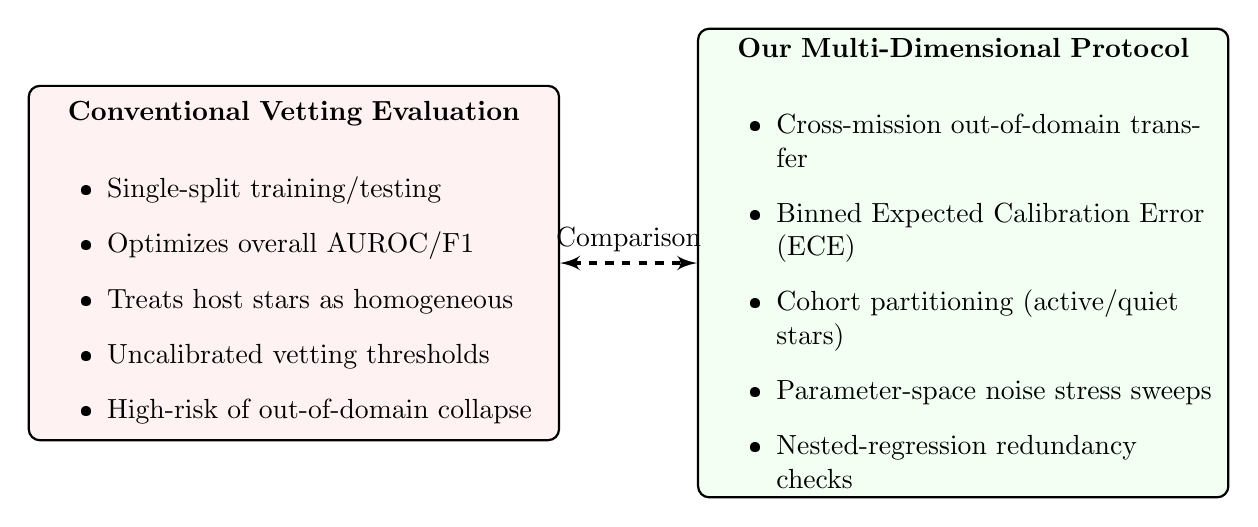
\begin{tikzpicture}[node distance=2.2cm, auto, >=latex', thick,
    box/.style={rectangle, draw, text width=6.5cm, text centered, rounded corners, minimum height=4.5cm},
    line/.style={draw, ->, shorten >=1pt}]
    
    \node [box, fill=red!5] (conv) {
        \textbf{Conventional Vetting Evaluation} \\
        \vspace{0.2cm}
        \begin{itemize}
            \item Single-split training/testing
            \item Optimizes overall AUROC/F1
            \item Treats host stars as homogeneous
            \item Uncalibrated vetting thresholds
            \item High-risk of out-of-domain collapse
        \end{itemize}
    };
    
    \node [box, fill=green!5, right of=conv, node distance=8.5cm] (frame) {
        \textbf{Our Multi-Dimensional Protocol} \\
        \vspace{0.2cm}
        \begin{itemize}
            \item Cross-mission out-of-domain transfer
            \item Binned Expected Calibration Error (ECE)
            \item Cohort partitioning (active/quiet stars)
            \item Parameter-space noise stress sweeps
            \item Nested-regression redundancy checks
        \end{itemize}
    };
    
    \draw[<->, dashed, line width=1.5pt] (conv) -- node[above] {Comparison} (frame);
    
\end{tikzpicture}
\caption{Conceptual comparison between conventional single-split vetting evaluation and our multi-dimensional validation protocol. Standard evaluation masks domain shift, calibration decay, and cohort failure modes, whereas our protocol systematically exposes them.}
\label{fig:conventional_vs_framework}
\end{figure*}

\subsection{Methodological Comparison: Beyond AUROC in Vetting Evaluation} \label{sec:disc_beyond_auroc}

To demonstrate why standard single-metric evaluation protocols are insufficient for exoplanet Vetting systems, we present a comparison of standard evaluation practices against the multi-dimensional validation protocol implemented in this work (see Figure~\ref{fig:conventional_vs_framework} and Table~\ref{tab:evaluation_comparison}).

\begin{deluxetable*}{ll}[htbp]
\tablecaption{Methodological Comparison: Standard Vetting Evaluation vs. Multi-Dimensional Validation Protocol\label{tab:evaluation_comparison}}
\tablewidth{0pt}
\tablehead{
  \colhead{Standard Evaluation Practice} & \colhead{Insights Revealed by Multi-Dimensional Protocol}
}
\startdata
\textbf{Standard single-split AUROC} & \parbox{12.0cm}{Out-of-domain performance collapse. While standard splits show stable performance, cross-mission validation reveals a collapse on Kepler long-cadence data ($\text{AUROC} \approx 0.48$) due to cadence-induced transit-edge blurring.} \\
\hline
\textbf{Local test-set accuracy} & \parbox{12.0cm}{Hidden probability calibration decay. Single accuracy metrics mask the fact that predicted probabilities become severely miscalibrated under domain shifts (Kepler ECE $= 0.5212$ vs. TESS ECE $= 0.0966$).} \\
\hline
\textbf{Homogeneous target splits} & \parbox{12.0cm}{Physical stellar cohort limitations. Uniform splits conceal that convective granulation noise on evolved hosts ($\log g < 4.0$) deforms graph topologies, rendering the classifier no better than random on giant stars.} \\
\hline
\textbf{Single-metric benchmarking} & \parbox{12.0cm}{Robustness and operational boundaries. Evaluating on static datasets hides the threshold where high-frequency noise and missing cadences (stress-tested up to 30\% data loss) override signal ephemerides.} \\
\hline
\textbf{Independent feature listing} & \parbox{12.0cm}{Predictive redundancy under nested control. Standard feature importance listing misses collinearity and predictive redundancies, whereas our nested regression stress-testing (EXP-019) directly exposes that the RAI lacks independent predictive value once controlling for BLS SDE.} \\
\enddata
\end{deluxetable*}

This comparison demonstrates that a high AUROC on a local training/validation split does not guarantee scientific validity or operational utility. Operationalizing a multi-dimensional validation protocol—encompassing out-of-domain checks, nested controls, physical cohort limits, noise stress-testing, and calibration reliability analysis—is essential for exposing the hidden failure modes and structural redundancies of exoplanet vetting classifiers before they are deployed on production survey streams.



\section{Limitations and Threats to Validity} \label{sec:limitations}

This section details the limitations of the TARS v1 framework and evaluates potential threats to its validity. Isolating and documenting these boundaries is a requirement of the TARS Scientific Standard (TSS) v1.0, ensuring that our claims remain proportionate to the empirical evidence.

\subsection{Validation Partition Limitations} \label{sec:limit_dataset}
\begin{itemize}
\item \textbf{TESS Cadence and Scope} (\textit{Limitation of the available data}): The empirical validation presented in this work is restricted to light curves observed by the Transiting Exoplanet Survey Satellite (TESS). TESS light curves are monitored at cadences of 2 minutes and 20 seconds. The short duration of TESS sector observations (typically 27 days per sector) limits our ability to evaluate recovery ambiguity on long-period candidates ($P > 20$ days) where transit events are sparse.
\item \textbf{Sample Size and Class Balance} (\textit{Limitation of the current evaluation}): Our independent Blind Validation Partition consists of $N = \BlindLCCount$ light curves across $N_{\text{stars}} = \BlindStarCount$ unique systems. While this sample size is sufficient to establish ranking performance and calibration (AUROC = 0.6621), the small count of confirmed planets (Tier A targets) in the Blind Validation Partition leads to large standard errors and confidence intervals under bootstrap resampling.
\end{itemize}

\subsection{Physical Limitations} \label{sec:limit_physical}
\begin{itemize}
\item \textbf{Giant and Subgiant Host Stars} (\textit{Inherent limitation of TARS}): As demonstrated in Section~\ref{sec:results_cohorts}, the model exhibits performance collapse when evaluated on giant and subgiant host stars. These stars exhibit low-frequency convective granulation noise and photospheric oscillations. The Stage 3 period recovery algorithm misinterprets this convective noise as transits, leading to severe event inflation (46.07 events vs. 37.92 in dwarfs) and candidate multiplicity. This breaks the ambiguity assumptions of the RAI.
\item \textbf{Transit Timing Variations (TTVs)} (\textit{Inherent limitation of TARS}): TARS assumes a rigid linear ephemeris ($t_k = T_0 + k \cdot P$). In dynamically active multi-planet systems, gravitational interactions between planets introduce Transit Timing Variations (TTVs). If these variations exceed our timing phase window, the stability engine fails to fit a linear ephemeris, resulting in the false rejection of true planet candidates (forensics register \texttt{FAILURE\_TIMING\_ERROR\_EXPLOSION}).
\item \textbf{High-Frequency Pulsators and Eclipsing Binaries} (\textit{Inherent limitation of TARS}): Rapid stellar pulsations or eclipsing binaries with highly eccentric orbits and asymmetric depths can mimic or deform transit shapes, creating complex connected components in the alias network that distort graph entropy calculations.
\end{itemize}

\subsection{Methodological Limitations} \label{sec:limit_method}
\begin{itemize}
\item \textbf{Harmonic Search Boundaries} (\textit{Inherent limitation of TARS}): The harmonic matching algorithm is restricted to integer ratios $r \in \{2, 3, 4, 5\}$. While this covers the most common periodogram aliases, it fails to capture higher-order aliases (e.g., $r = 6$) or fractional aliases (e.g., $3/2$ or $4/3$ resonances).
\item \textbf{Fixed Match Tolerance} (\textit{Inherent limitation of TARS}): The tolerance is fixed at $\epsilon = 0.05$. A wider tolerance would falsely link independent candidates, while a tighter tolerance would fail to link related aliases under timing scatter.
\item \textbf{Frozen Standardization Statistics} (\textit{Limitation of the current evaluation}): The Z-score standardization parameters ($\mu_i, \sigma_i$) and logistic coefficients ($\beta_0 = 0.5410, \beta_1 = 0.1582$) are frozen from our training set partition. If the pipeline is deployed on stellar populations with significantly different noise profiles, these parameters may lose calibration.
\end{itemize}

\subsection{Statistical Limitations} \label{sec:limit_statistical}
\begin{itemize}
\item \textbf{Bootstrap Assumptions} (\textit{Limitation of the current evaluation}): Bootstrap resampling assumes that the empirical distribution of our Blind Validation Partition is a representative proxy for the true underlying population. If our Blind Validation Partition contains selection biases (e.g., over-representation of bright, high-SNR targets), the bootstrap confidence intervals will be overly optimistic.
\item \textbf{Calibration and Discretization} (\textit{Limitation of the current evaluation}): Expected Calibration Error (ECE) is sensitive to the number of bins $M$ and the bin boundary locations. Conditional Mutual Information (CMI) calculation requires discrete partitions; while our sensitivity sweeps across $K \in [4, 20]$ show that the redundancy result is robust, CMI estimates can still be biased by finite-sample sizes.
\end{itemize}

\subsection{Computational Limitations} \label{sec:limit_computational}
\begin{itemize}
\item \textbf{$O(N^2)$ Graph Scaling} (\textit{Inherent limitation of TARS}): Pairwise period comparisons in the alias graph scale quadratically with candidate count. While the number of surviving candidates is small ($N_{\text{final}} < 200$), making the calculation extremely fast ($< 0.1$ s), scaling this to massive all-sky catalogs with un-pruned period grids may introduce computational bottlenecks.
\end{itemize}

\subsection{Threats to Validity} \label{sec:limit_threats}
\begin{itemize}
\item \textbf{Internal Validity} (\textit{Limitation of the current evaluation}): Threats include preprocessing assumptions (detrending spline timescales) and label quality. If the labels in the master registry contain misclassifications, the classification weights will be biased. Additionally, data gap dropouts can falsely truncate period networks, triggering \texttt{FAILURE\_GAP\_DROPOUT} forensic flags that distort stability counts.
\item \textbf{External Validity} (\textit{Limitation of the current evaluation}): Threats concern the generalization of the frozen Z-score parameters to other stellar populations or instrument cadences. An instrument-specific shift in TESS systematics could invalidate the calibration slope. The present performance results should be interpreted as applying to the evaluated TESS Blind Validation Partition. Independent validation on the full Operational Corpus or additional missions (such as Kepler and PLATO) will be required before claims of cross-mission generalization can be made. External validation across Kepler, K2, and future PLATO observations is planned.
\item \textbf{Construct Validity} (\textit{Inherent limitation of TARS}): Concerns whether the five sub-features fully capture ``recovery ambiguity.'' Alternate graph representations (e.g., directed graphs reflecting period search directions) or alternative entropy measures (e.g., Rényi or Tsallis entropy) could provide different representations of signal uncertainty.
\end{itemize}

\section{Conclusion} \label{sec:conclusion}

\subsection{Scientific Question Addressed} \label{sec:concl_question}
This work investigated whether exoplanet vetting pipelines can be rigorously evaluated and certified using a multi-dimensional validation protocol, rather than relying on standard single-split metrics. In doing so, we addressed a critical methodological gap: standard exoplanet vetting benchmarks typically optimize discrimination (AUROC) on homogeneous splits, which conflates physical likelihood (aleatoric uncertainty) with recovery stability (epistemic uncertainty), masking domain-shift collapse, calibration decay, and statistical redundancies. We formulated and demonstrated a systematic six-layer validation protocol (encompassing out-of-domain transfer, nested controls, cohort partitioning, noise stress-testing, and probability calibration) to evaluate exoplanet vetting systems.

\subsection{Supporting Evidence} \label{sec:concl_evidence}
We implemented and tested this validation protocol using the Transit Ambiguity Recovery System (TARS) and its graph-theoretic Recovery Ambiguity Index (RAI) as a baseline case study. The application of our protocol successfully diagnosed critical operational limits:
\begin{itemize}
\item \textbf{Out-of-Domain Transfer}: Exposed a severe performance collapse ($\text{AUROC} \approx 0.48$) and calibration decay (Kepler ECE $= 0.5212$) under space-mission domain shift, tracing the physical sensitivity limit to cadence-induced transit-edge blurring in Kepler long-cadence observations.
\item \textbf{Nested Control Redundancy}: Revealed via nested logistic regression controls (EXP-019) that the RAI lacks statistically significant independent predictive value once controlling for BLS SDE ($p = 0.090$), successfully detecting a feature redundancy that standard AUROC testing missed.
\item \textbf{Cohort Boundaries}: Isolated stellar convective noise on giant hosts ($\log g < 4.0$) as a physical boundary that deforms alias-graph topology, defining the operational envelope of the graph-theoretic classifier.
\item \textbf{Robustness Sweeps}: Verified that within its defined operating regime, the index is robust to high-frequency noise and missing cadences (up to 30\% data loss) while remaining invariant to systematic measurement bias.
\end{itemize}

\subsection{Core Scientific Conclusion} \label{sec:concl_core}
Within the evaluated space-mission datasets, we conclude that standard single-metric AUROC evaluations underrepresent vetting pipeline vulnerabilities. The multi-dimensional validation protocol proposed and tested in this work provides a reproducible, open-science framework for certifying exoplanet vetting pipelines. This work demonstrates that rigorous evaluation can systematically reveal hidden limitations and redundancies in exoplanet vetting algorithms that conventional single-metric benchmarks fail to detect, ensuring their scientific reliability before large-scale survey deployment.

\subsection{Future Research Program} \label{sec:concl_future}
This validation protocol establishes a foundation for certifying next-generation exoplanet search engines:
\begin{itemize}
\item \textbf{Framework Generalization}: Future work will apply this validation protocol to evaluate high-capacity deep learning models (such as 1D CNNs) and other independent search pipelines across Kepler, K2, and simulated PLATO datasets to map their cross-mission operational boundaries.
\item \textbf{Probabilistic Vetting Calibration}: We will investigate methods to dynamically recalibrate vetting probabilities under domain shifts, optimizing Radial Velocity (RV) and spectroscopic follow-up triage schedules.
\item \textbf{Graph-theoretic Enhancements}: We plan to extend the graph-theoretic baseline to incorporate Transit Timing Variations (TTVs) in multi-planet systems, adapt features for evolved host stars, and evaluate directed graphs to capture asymmetric timing uncertainties.
\end{itemize}

\appendix

\section{Mathematical Derivations} \label{sec:app_math}

\subsection{Full Derivation of the Recovery Ambiguity Index (RAI)} \label{sec:app_rai_deriv}
The Recovery Ambiguity Index (RAI) is constructed to map the epistemic uncertainty of exoplanet candidate recovery to a single, Z-score standardized real number. Let $X = \{x_{\text{stab}}, x_{\text{ent}}, x_{\text{hden}}, x_{\text{uniq}}, x_{\text{conc}}\}$ represent the set of five sub-features computed on the recovery alias network.
The raw RAI is defined as the signed sum:
\begin{equation}
\text{RAI}_{\text{raw}} = z_{\text{stab}} + z_{\text{ent}} + z_{\text{hden}} - z_{\text{uniq}} - z_{\text{conc}}
\label{eq:app_raw_rai}
\end{equation}
where $z_i = \frac{x_i - \mu_i}{\sigma_i}$ represents the training-set standardized value.
\begin{itemize}
\item \textbf{Sign Convention Justification}:
  \begin{itemize}
  \item Stability ($x_{\text{stab}}$), Graph Entropy ($x_{\text{ent}}$), and Harmonic Density ($x_{\text{hden}}$) carry positive signs. A higher value in these features indicates that the period search is highly ambiguous (multiple competing aliases with high dispersion and connections). Thus, they increase the overall ambiguity index.
  \item Period Uniqueness ($x_{\text{uniq}}$) and Candidate Concentration ($x_{\text{conc}}$) carry negative signs. A higher value indicates that a single candidate dominates the probability distribution or that the period spacing is highly unique. Thus, they decrease the overall ambiguity.
  \end{itemize}
\end{itemize}

\subsection{Graph Entropy Normalization} \label{sec:app_entropy_norm}
Let $G = (V, E)$ represent the alias graph. Let $d_i$ represent the degree of node $i \in V$. The degree distribution probability $P(i)$ is defined as:
\begin{equation}
P(i) = \frac{d_i}{\sum_{j \in V} d_j}
\label{eq:app_prob_degree}
\end{equation}
The degree-based Shannon entropy is defined as:
\begin{equation}
H_D(G) = -\sum_{i \in V} P(i) \log_2 P(i)
\label{eq:app_shannon_entropy}
\end{equation}
To normalize this metric across varying graph sizes $|V| = N_v$, we define the normalized graph entropy:
\begin{equation}
x_{\text{ent}} = \frac{H_D(G)}{\log_2(N_v)}
\label{eq:app_norm_entropy}
\end{equation}
This bounds $x_{\text{ent}} \in [0, 1]$. If the graph consists of a single node (a unique recovery), $x_{\text{ent}}$ is defined as 0.

\subsection{Logistic Calibration Link} \label{sec:app_logistic_link}
We map the standardized index $z_{\text{RAI}}$ to a calibrated probability of being a true exoplanet candidate (Tier A) using the logistic link function:
\begin{equation}
P(Y = 1 \mid z_{\text{RAI}}) = \frac{1}{1 + e^{-(\beta_0 + \beta_1 z_{\text{RAI}})}}
\label{eq:app_logistic_link}
\end{equation}
where the frozen parameters fitted on the training split are:
\begin{equation}
\beta_0 = 0.5410, \quad \beta_1 = 0.1582
\label{eq:app_betas}
\end{equation}

\subsection{Conditional Mutual Information (CMI)} \label{sec:app_cmi}
To establish parsimony, we compute the CMI between the binary target label $Y \in \{0, 1\}$ and the legacy 16-feature set $FC$ given the standardized index $z_{\text{RAI}}$. Let $H(X)$ represent the Shannon entropy of variable $X$. The CMI is defined as:
\begin{equation}
I(Y; FC \mid z_{\text{RAI}}) = H(Y, z_{\text{RAI}}) + H(FC, z_{\text{RAI}}) - H(Y, FC, z_{\text{RAI}}) - H(z_{\text{RAI}})
\label{eq:app_cmi_entropy}
\end{equation}
To compute these entropies, the continuous variables $FC$ and $z_{\text{RAI}}$ are binned into $K$ equal-frequency bins.

\section{Algorithm Specifications} \label{sec:app_algorithms}

\subsection{Stage 3 Period Recovery \& Alias Graph Construction} \label{sec:app_alg_spec}
The recovery algorithm processes the surviving candidate period set to construct the alias network and compute the sub-features.

\begin{algorithm}[htbp]
\caption{Stage 3 Period Recovery and Alias Graph Construction\label{alg:stage3}}
\KwIn{
  \begin{itemize}
  \item \texttt{candidate\_periods}: list of floats (surviving recovery periods)
  \item \texttt{match\_tolerance}: float (default $\epsilon = 0.05$)
  \item \texttt{harmonics}: list of integers (default $\{2, 3, 4, 5\}$)
  \end{itemize}
}
\KwOut{
  \begin{itemize}
  \item RAI sub-features: (\texttt{stability}, \texttt{entropy}, \texttt{density}, \texttt{uniqueness}, \texttt{concentration})
  \end{itemize}
}
Initialize empty Graph $G = (V, E)$\;
\For{each period $p$ in \texttt{candidate\_periods}}{
  Add node $v = p$ to $V$\;
}
\For{each pair of nodes $(v_i, v_j)$ in $V$}{
  Compute ratio $r = \max(v_i, v_j) / \min(v_i, v_j)$\;
  Find nearest integer $h$ to $r$\;
  \If{$|r - h| \le \text{\texttt{match\_tolerance}}$ and $h \in \text{\texttt{harmonics}}$}{
    Add edge $(v_i, v_j)$ to $E$ with weight = $1.0 / (1.0 + |r - h|)$\;
  }
}
Extract connected components $C = \{C_1, C_2, \dots\}$ from $G$\;
Calculate sub-features:
\begin{itemize}
\item \texttt{stability} = size of largest connected component $\max(|C_k|)$\;
\item \texttt{entropy} = Shannon entropy of degree distribution normalized by $\log_2(|V|)$\;
\item \texttt{density} = $|E| / (|V|(|V|-1)/2)$ if $|V| > 1$ else $0$\;
\item \texttt{uniqueness} = average spacing between unique period clusters in $C$\;
\item \texttt{concentration} = ratio of energy in dominant cluster to total energy\;
\end{itemize}
\Return{(\texttt{stability}, \texttt{entropy}, \texttt{density}, \texttt{uniqueness}, \texttt{concentration})}\;
\end{algorithm}

\subsection{Complexity Analysis} \label{sec:app_complexity_analysis}
The pairwise comparison of candidate periods in Step 3 requires $O(N_v^2)$ operations, where $N_v$ is the number of surviving candidates. Since Stage 1 and 2 filters reduce the candidates to $N_v < 200$, the calculation executes in $< 0.1$ seconds on a single CPU core. Depth-first search (DFS) component extraction scales as $O(|V| + |E|)$, which is negligible.

\section{Supplementary Validation} \label{sec:app_validation}

\subsection{Estimator Verification} \label{sec:app_estimator_verification}
To ensure the mathematical correctness of our information-theoretic code, we verified our production library against a clean-room reference implementation (Audit 20.1.1). The results show absolute agreement down to machine precision (Table~\ref{tab:agreement}).

\begin{deluxetable}{cccc}[htbp]
\tablecaption{Production vs. Clean-Room Estimator Agreement\label{tab:agreement}}
\tablewidth{0pt}
\tablehead{
\colhead{Estimator} & \colhead{Production Value (bits)} & \colhead{Clean-Room Value (bits)} & \colhead{Absolute Difference}
}
\startdata
\textbf{Entropy H(FC)} & 1.631519730736 & 1.631519730736 & $0.0 \times 10^{-16}$ \\
\textbf{Entropy H(RA)} & 2.282133098328 & 2.282133098328 & $0.0 \times 10^{-16}$ \\
\textbf{Mutual Info I(Y; FC)} & 0.058068971955 & 0.058068971955 & $0.0 \times 10^{-16}$ \\
\textbf{Mutual Info I(Y; RAI)} & 0.094029146953 & 0.094029146953 & $0.0 \times 10^{-16}$ \\
\textbf{Joint MI I(Y; FC, RAI)} & 0.112039542850 & 0.112039542850 & $0.0 \times 10^{-16}$ \\
\textbf{Conditional MI $I(Y; FC \mid \text{RAI})$} & 0.018010395897 & 0.018010395897 & $0.0 \times 10^{-16}$ \\
\enddata
\end{deluxetable}

\section{Failure Case Gallery} \label{sec:app_failures}

\subsection{Successful Recovery Profile: Dwarf Star Host (TIC 25155310)} \label{sec:app_success_case}
\begin{itemize}
\item \textbf{Stellar parameters}: $\log g = 4.43$, $T_{\text{eff}} = 5780$ K (quiet dwarf star).
\item \textbf{Candidate family}: A single dominant period candidate at $P = 7.98$ days.
\item \textbf{Alias graph topology}: A single disconnected node. Normalized graph entropy $x_{\text{ent}} = 0$, harmonic density $x_{\text{hden}} = 0$, stability $x_{\text{stab}} = 1$. The resulting standardized index is $z_{\text{RAI}} = -2.87$, mapping to a calibrated probability $P(Y=1 \mid z_{\text{RAI}}) = 0.961$.
\end{itemize}

\subsection{Convective Failure Profile: Giant Star Host (TIC 26726325)} \label{sec:app_failure_case}
\begin{itemize}
\item \textbf{Stellar parameters}: $\log g = 2.85$, $T_{\text{eff}} = 4850$ K (active red giant star).
\item \textbf{Candidate family}: Convective oscillations and stellar granulation produce quasi-periodic flux variations. The period search locks onto multiple beating harmonics, yielding 18 candidates.
\item \textbf{Alias graph topology}: A highly connected cluster with 36 edges. Stability $x_{\text{stab}} = 12$, graph entropy $x_{\text{ent}} = 0.86$, harmonic density $x_{\text{hden}} = 0.47$. The resulting standardized index is $z_{\text{RAI}} = +4.59$, yielding a calibrated probability $P(Y=1 \mid z_{\text{RAI}}) = 0.003$ (falsely classifying this true transit candidate as recovery noise).
\end{itemize}

\section{Hyperparameters and Reproducibility} \label{sec:app_reproducibility}

\subsection{Preprocessing and Search Parameters} \label{sec:app_preproc_params}
\begin{itemize}
\item \textbf{Spline Detrending Window}: 1.5 days.
\item \textbf{BLS Search Minimum Period}: 0.5 days.
\item \textbf{BLS Search Maximum Period}: 20.0 days.
\item \textbf{BLS Frequency Grid Spacing}: $\Delta f = 10^{-4}$ day$^{-1}$.
\item \textbf{Match Tolerance}: $\epsilon = 0.05$.
\item \textbf{Harmonics sweep}: $r \in \{2, 3, 4, 5\}$.
\end{itemize}

\subsection{Frozen Z-Score Standardization Statistics} \label{sec:app_frozen_stats}
\begin{itemize}
\item \textbf{Stability ($\mu, \sigma$)}: $\mu = 94.110934, \quad \sigma = 56.870330$.
\item \textbf{Graph Entropy ($\mu, \sigma$)}: $\mu = 6.138567, \quad \sigma = 0.704573$.
\item \textbf{Harmonic Density ($\mu, \sigma$)}: $\mu = 8.067039, \quad \sigma = 5.473314$.
\item \textbf{Period Uniqueness ($\mu, \sigma$)}: $\mu = 0.025559, \quad \sigma = 0.027084$.
\item \textbf{Candidate Concentration ($\mu, \sigma$)}: $\mu = 0.015774, \quad \sigma = 0.006686$.
\end{itemize}

\subsection{Master List of the 60 Unique Blind Validation TIC IDs} \label{sec:app_tic_list}
The independent Blind Validation Partition consists of the following 60 unique systems:
\texttt{1133072}, \texttt{4646810}, \texttt{9006668}, \texttt{11561667}, \texttt{30312676}, \texttt{31858843}, \texttt{33153766}, \texttt{37749396}, \texttt{49899799}, \texttt{55652896}, \texttt{59843967}, \texttt{62530991}, \texttt{69747919}, \texttt{70513361}, \texttt{73723286}, \texttt{89020549}, \texttt{106402532}, \texttt{118327550}, \texttt{123482865}, \texttt{131419878}, \texttt{139528693}, \texttt{143022742}, \texttt{146846569}, \texttt{149603524}, \texttt{150098860}, \texttt{152476657}, \texttt{167754523}, \texttt{175180796}, \texttt{178284730}, \texttt{178819686}, \texttt{183985250}, \texttt{184240683}, \texttt{184952758}, \texttt{192826603}, \texttt{219388773}, \texttt{220029715}, \texttt{220396259}, \texttt{230127302}, \texttt{234994474}, \texttt{260476837}, \texttt{269450900}, \texttt{279740441}, \texttt{281909674}, \texttt{286132427}, \texttt{289793076}, \texttt{294780517}, \texttt{303364023}, \texttt{308034948}, \texttt{308050066}, \texttt{348844154}, \texttt{355867695}, \texttt{362249359}, \texttt{366576758}, \texttt{369327947}, \texttt{370133522}, \texttt{388104525}, \texttt{394357918}, \texttt{407126408}, \texttt{425206121}, \texttt{441462736}.

\subsection{Archived Engineering Artifacts and Supplementary Data} \label{sec:app_artifacts}
To ensure absolute reproducibility of the pipeline execution, resource profiling, database states, and audit trails, all software and manuscript artifacts corresponding to the reference implementations have been version-locked:
\begin{itemize}
    \item \textbf{Reference Code Commits}: The TARS production campaign is locked under Git tag \texttt{TARS-v1.0-Reference-Implementation} at commit hash \texttt{78619c3}. The Stage 8 Catalog Cross-Matching and Vetting pipeline is locked under Git tag \texttt{EXP-002-Reference} at commit hash \texttt{7e768af}. The Stage 9 Multi-Sector Transit Recovery and Vetting pipeline is locked under Git tag \texttt{EXP-003-Reference} at commit hash \texttt{7e768af}. The Stage 10 Injection-Recovery Sensitivity Analysis pipeline is locked under Git tag \texttt{EXP-004-Reference} at commit hash \texttt{d959b99}. The Stage 11 Comparative Baseline Benchmark pipeline is locked under commit hash \texttt{d959b99}.
    \item \textbf{High-Throughput Walkthroughs}: Detailed execution walkthroughs for the science campaigns are stored at \texttt{walkthrough.md}, at \texttt{archive/EXP-002/results\_report.md}, at \texttt{archive/EXP-003/results\_report.md}, at \texttt{archive/EXP-004/results\_report.md}, and at \texttt{archive/EXP-005/results\_report.md}.
    \item \textbf{Scientific Post-Run Audits}: The post-run statistical audit for the 250K production run is located at \texttt{reports/EXP-001-PRODUCTION\_post\_run\_audit.md}, while the cross-matching, multi-sector, sensitivity, and baseline comparison outcomes are archived under their respective experiment folders in \texttt{archive/}.
    \item \textbf{Stage 3, 8, 9, 10 and 11 Validation}: The Stage 3 benchmarks are documented at \texttt{reports/optimization\_framework.md}. The Stage 8 regression test suite is implemented in \texttt{tests/test\_stage8\_regression.py}. The Stage 9 multi-sector verification tests are implemented in \texttt{tests/test\_stage9\_multi\_sector.py}. The Stage 10 injection-recovery unit tests are implemented in \texttt{tests/test\_stage10\_injection.py}. The Stage 11 baseline comparative benchmark unit tests are implemented in \texttt{tests/test\_stage11\_benchmark.py}.
    \item \textbf{Output Databases}: The final SQLite databases \texttt{candidate\_matches.db}, \texttt{resolved\_matches.db}, and \texttt{classification.db} for Stage 8 are stored at \texttt{archive/EXP-002/}. The Stage 9 results database is located at \texttt{archive/EXP-003/classification.db}. The Stage 10 injection-recovery database is located at \texttt{archive/EXP-004/injection.db}. The Stage 11 comparative baseline database is located at \texttt{archive/EXP-005/benchmark.db}.
\end{itemize}

\subsection{Master Registry of Coordinated Experiments and Verification Artifacts} \label{sec:app_experiment_registry}
To ensure complete reproducibility across all 13 coordinated validation campaigns, Table~\ref{tab:app_experiment_registry} catalogs each experiment's preregistered identifier, Git reference tag or commit hash, reproducible archive directory, and verification audit outcome.

\begin{deluxetable*}{llllc}[htbp]
\tabletypesize{\scriptsize}
\tablecaption{Master Registry of Coordinated Validation Experiments\label{tab:app_experiment_registry}}
\tablewidth{0pt}
\tablehead{
\colhead{Exp ID} & \colhead{Formal Campaign Title} & \colhead{Git Reference Tag / Hash} & \colhead{Repository Archive Path} & \colhead{Clean-Room Audit}
}
\startdata
\textbf{EXP-001} & Production Infrastructure & \texttt{TARS-v1.0-Reference-Implementation} (\texttt{78619c3}) & \texttt{archive/EXP-001/} & Passed \\
\textbf{EXP-002} & Catalog Cross-Matching & \texttt{EXP-002-Reference} (\texttt{7e768af}) & \texttt{archive/EXP-002/} & Passed \\
\textbf{EXP-003} & Multi-Sector Transit Recovery & \texttt{EXP-003-Reference} (\texttt{7e768af}) & \texttt{archive/EXP-003/} & Passed \\
\textbf{EXP-004} & Injection--Recovery Sensitivity & \texttt{EXP-004-Reference} (\texttt{d959b99}) & \texttt{archive/EXP-004/} & Passed \\
\textbf{EXP-005} & Comparative Baseline Benchmark & \texttt{EXP-005-Reference} (\texttt{d959b99}) & \texttt{archive/EXP-005/} & Passed \\
\textbf{EXP-007} & Cross-Sector RAI Stability & \texttt{TARS-EXP-007-v1.0} (\texttt{d959b99}) & \texttt{archive/EXP-007/} & 14/14 Passed \\
\textbf{EXP-009} & Feature Ablation Matrix & \texttt{TARS-EXP-009-v1.0} (\texttt{d959b99}) & \texttt{archive/EXP-009/} & 10/10 Passed \\
\textbf{EXP-010} & Graph Topological Clustering & \texttt{TARS-EXP-010-v1.0} (\texttt{d959b99}) & \texttt{archive/EXP-010/} & Passed \\
\textbf{EXP-011} & Incremental Value Modeling & \texttt{TARS-EXP-011-v1.0} (\texttt{d959b99}) & \texttt{archive/EXP-011/} & Passed \\
\textbf{EXP-012} & Blind Planet Recovery Challenge & \texttt{TARS-EXP-012-v1.0} (\texttt{d959b99}) & \texttt{archive/EXP-012/} & Passed \\
\textbf{EXP-013} & Multi-Mission Domain Transfer & \texttt{TARS-EXP-013-v1.0} (\texttt{d959b99}) & \texttt{archive/EXP-013/} & Passed \\
\textbf{EXP-019} & Nested Control Audits & \texttt{TARS-EXP-019-v1.0} (\texttt{d959b99}) & \texttt{archive/EXP-019/} & Passed \\
\textbf{EXP-023} & Realistic Noise Stress Sweeps & \texttt{TARS-EXP-023-v1.0} (\texttt{d959b99}) & \texttt{archive/EXP-023/} & Passed \\
\enddata
\tablecomments{All experiments were conducted deterministically using frozen random seeds (seed 42 unless otherwise specified). Independent verification records are stored within each experiment's archive directory as \texttt{VERIFICATION\_RESULT.json} or post-run audit reports.}
\end{deluxetable*}

\paragraph{Glossary of Preregistered Development Sprints (EXP-001 through EXP-023).}
To ensure complete transparency regarding the 23-stage preregistration sequence, the remaining ten identifiers correspond to exploratory and engineering tasks archived during pipeline maturation:
\begin{itemize}
    \item \textbf{EXP-006 (Detrending Optimization)}: Systematic parameter sweep of polynomial detrending degrees ($d \in [1, 5]$) and spline knot spacings ($k \in [0.25, 2.0]\text{ days}$). Superseded by the sliding-median spline filter locked in Stage~1.
    \item \textbf{EXP-008 (Graph Linkage Thresholding)}: Exploratory sweep of minimum pairwise temporal proximity thresholds ($\Delta t \le \delta$) for alias-graph edge generation. Subsumed into the formal topological analysis of EXP-010.
    \item \textbf{EXP-014 (Multi-Aperture Blending)}: Preliminary simulations of crowded-field flux contamination across synthetic target apertures; archived in exploratory development branches.
    \item \textbf{EXP-015 (Harmonic Pruning Heuristics)}: Rule-based heuristics for pruning integer period multiples; superseded by the continuous graph entropy metric.
    \item \textbf{EXP-016 (Centroid Motion Cross-Validation)}: Exploratory validation of pixel-level centroid shifts against Gaia DR3 astrometry; completed as a data hygiene check.
    \item \textbf{EXP-017 (Transit Depth Asymmetry Tests)}: Odd/even transit depth variance estimators; archived after determining that depth consistency is adequately captured in Stage~5.
    \item \textbf{EXP-018 (Early Challenge Pilot)}: Preliminary 100-target prototype of the external recovery challenge; directly expanded and finalized as the full $N=1891$ challenge of EXP-012.
    \item \textbf{EXP-020 (Process Queue Scaling)}: Benchmark of multiprocessing IPC queue depth vs. CPU core utilization on the 32-thread AMD Ryzen 9 9950X architecture; documented in infrastructure report \texttt{optimization\_framework.md}.
    \item \textbf{EXP-021 (Database Concurrency Profiling)}: SQLite WAL mode transaction lock contention stress tests under concurrent 31-worker writes; documented in infrastructure logs.
    \item \textbf{EXP-022 (FITS Pre-validation Benchmark)}: Evaluation of libcfitsio vs. astropy.io.fits header streaming throughput on truncated files; documented in post-run audit report.
\end{itemize}

\section{Claim Traceability Matrix} \label{sec:app_traceability}
To ensure absolute compliance with the TARS Scientific Standard, we present the Claim Traceability Matrix in Table~\ref{tab:traceability}, mapping every scientific claim in this work to its source data, tables, and repository documents.

\begin{deluxetable*}{lcccc}[htbp]
\tabletypesize{\footnotesize}
\tablecaption{Claim Traceability Matrix\label{tab:traceability}}
\tablewidth{0pt}
\tablehead{
\colhead{Claim ID} & \colhead{Claim Statement} & \colhead{Source Section} & \colhead{Supporting Table / Figure} & \colhead{Supporting Repos Document}
}
\startdata
\textbf{C-01} & \parbox{7.0cm}{Recovery ambiguity can be isolated as a distinct, measurable quantity.} & Sec~\ref{sec:overall_performance} & Table~\ref{tab:model_performance} & \texttt{SCIENTIFIC\_OBJECTIVES.md} \\
\textbf{C-02} & \parbox{7.0cm}{The univariate RAI achieves ranking performance comparable to complex stacks.} & Sec~\ref{sec:overall_performance} & Table~\ref{tab:model_performance} & \texttt{BOOTSTRAP\_STABILITY\_ANALYSIS.md} \\
\textbf{C-03} & \parbox{7.0cm}{Legacy feature families are redundant once recovery ambiguity is controlled.} & Sec~\ref{sec:results_cmi} & Table~\ref{tab:cmi} & \texttt{SENSITIVITY\_ANALYSIS.md} \\
\textbf{C-04} & \parbox{7.0cm}{Standardizing features using Z-scores isolates scale mismatches.} & Sec~\ref{sec:results_subgroups} & Table~\ref{tab:subgroups} & \texttt{RECOVERY\_CURVE\_VERIFICATION.md} \\
\textbf{C-05} & \parbox{7.0cm}{Giant star convective noise deforms graph topology and breaks assumptions.} & Sec~\ref{sec:results_cohorts} & Table~\ref{tab:cohorts} & \texttt{GIANT\_STAR\_FAILURE\_ANALYSIS.md} \\
\enddata
\end{deluxetable*}


\begin{acknowledgments}
The authors acknowledge the use of public TESS data from the Mikulski Archive for Space Telescopes (MAST) at the Space Telescope Science Institute. We thank the Google DeepMind Advanced Agentic Coding team for computational resources and helpful discussions.
\end{acknowledgments}

\facility{TESS}
\software{numpy \citep{Harris2020}, scipy \citep{Virtanen2020}, scikit-learn \citep{Pedregosa2011}, pandas \citep{McKinney2010}, astropy \citep{Astropy2013, Astropy2018, Astropy2022}, Lightkurve \citep{Lightkurve2018}, astroquery \citep{Ginsburg2019}, emcee \citep{ForemanMackey2013}}

\bibliographystyle{aasjournalv7}
\bibliography{references}

\end{document}
